%%%%%%%%%%%%%%%%%%%%%%%%%%%%%%%%%%%%%%%%%%%%%%%%%%%%%%%%%%%%%%%%%%%%%%%%%%%%%%%%
%                                                                              %
%   PAW Guide/ Reference Manual -- LaTeX Source                                %
%                                                                              %
%   Main driver file. Includes other files of manual,                          %
%   generates table of contents and includes index file.                       %
%                                                                              %
%   To run, you need the CERN style  cernman.sty                               %
%                                                                              %
%   Editor: Michel Goossens / IT-ASD                                           %
%   Last Mod.: 30 July 1998  Olivier Couet                                     %
%                                                                              %
%%%%%%%%%%%%%%%%%%%%%%%%%%%%%%%%%%%%%%%%%%%%%%%%%%%%%%%%%%%%%%%%%%%%%%%%%%%%%%%%
\documentclass[10pt]{cernman}
\usepackage{fancyvrb}
\usepackage{pawdefs}
\usepackage{longtable}
\usepackage[dvips]{rotating}
\let\finalnewpage\clearpage
\let\finalclearpage\clearpage
\graphicspath{{../epsfiles/}}
\setlongtables
\renewcommand{\textfraction}{.05}
\renewcommand{\topfraction}{.95}
\renewcommand{\floatpagefraction}{.80}
\setcounter{totalnumber}{4}
\setcounter{topnumber}{3}
\makeindex
\DefineVerbatimEnvironment{alltt}{Verbatim}%
                          {fontsize=\small,commandchars=\\\{\},%
                           xleftmargin=0pt}
\DefineVerbatimEnvironment{falltt}{Verbatim}%
                          {fontsize=\footnotesize,commandchars=\\\{\},%
                           xleftmargin=0pt}
\DefineVerbatimEnvironment{salltt}{Verbatim}%
                          {fontsize=\scriptsize,commandchars=\\\{\},%
                           xleftmargin=0pt}
\DefineVerbatimEnvironment{talltt}{Verbatim}%
                          {fontsize=\tiny,commandchars=\\\{\},%
                           xleftmargin=0pt}
\DefineVerbatimEnvironment{verbatim}{Verbatim}%
                          {fontsize=\small,xleftmargin=0pt}
\begin{document}
%  ==================== Front material ============================

%%%%%%%%%%%%%%%%%%%%%%%%%%%%%%%%%%%%%%%%%%%%%%%%%%%%%%%%%%%%%%%%%%%
%                                                                 %
%   PAW   - Reference Manual -- LaTeX Source                      %
%                                                                 %
%   Front Material: Title page,                                   %
%                   Copyright Notice                              %
%                   Preliminary Remarks                           %
%                   Table of Contents                             %
%   EPS file      : cernlogo.eps                                  %
%                                                                 %
%   Editor: Michel Goossens / CN-AS                               %
%   Last Mod.: 16 August 1993 09:00 mg                            %
%                                                                 %
%%%%%%%%%%%%%%%%%%%%%%%%%%%%%%%%%%%%%%%%%%%%%%%%%%%%%%%%%%%%%%%%%%%
 
%%%%%%%%%%%%%%%%%%%%%%%%%%%%%%%%%%%%%%%%%%%%%%%%%%%%%%%%%%%%%%%%%%%%
%    Title page                                                    %
%%%%%%%%%%%%%%%%%%%%%%%%%%%%%%%%%%%%%%%%%%%%%%%%%%%%%%%%%%%%%%%%%%%%
\def\Ptitle#1{\special{ps: /Printstring (#1) def}
\epsfbox{cnastit.eps}}
 
\begin{titlepage}
\vspace*{-23mm}
\mbox{\epsfysize30mm\epsfbox{cern15.eps}}
\hfill
\raise8mm\hbox{\Large\bf CERN Program Library Long Writeup Q121}
\hfill\mbox{}
\begin{center}
\mbox{}\\[10mm]
\mbox{\Ptitle{PAW}}\\[2cm]
{\Huge Physics Analysis Workstation}\\[2cm]
{\Huge User's guide}\\[5cm]
%%%{\Large Application Software Group}\\[3mm]
{\Large Information Technology Division}\\[2cm]
\end{center}
\vfill
\begin{center}\Large CERN, Geneva, Switzerland\end{center}
\end{titlepage}
 
%%%%%%%%%%%%%%%%%%%%%%%%%%%%%%%%%%%%%%%%%%%%%%%%%%%%%%%%%%%%%%%%%%%%
%    Copyright  page                                               %
%%%%%%%%%%%%%%%%%%%%%%%%%%%%%%%%%%%%%%%%%%%%%%%%%%%%%%%%%%%%%%%%%%%%

\thispagestyle{empty}
\framebox[\textwidth][t]{\hfill\begin{minipage}{0.96\textwidth}%
\vspace*{3mm}\begin{center}Copyright Notice\end{center}
\parskip\baselineskip
{\bf PAW -- Physics Analysis Workstation}
 
CERN Program Library entry {\bf Q121}
 
\copyright{} Copyright CERN, Geneva 1992--1999
 
Copyright and any other appropriate legal protection of these
computer programs and associated documentation reserved in all
countries of the world.
 
These programs or documentation may not be reproduced by any
method without prior written consent of the Director-General
of CERN or his delegate.
 
Permission for the usage of any programs described herein is
granted apriori to those scientific institutes associated with
the CERN experimental program or with whom CERN has concluded
a scientific collaboration agreement.
 
Requests for information should be addressed to:
\vspace*{-.5\baselineskip}
\begin{center}
\tt\begin{tabular}{l}
CERN Program Library Office              \\
CERN-IT Division                         \\
CH-1211 Geneva 23                        \\
Switzerland                              \\
Tel.      +41 22 767 4951                \\
Fax.      +41 22 767 8630                \\
Internet: cernlib@cern.ch
\end{tabular}
\end{center}
\vspace*{2mm}
\end{minipage}\hfill}%end of minipage in framebox
\vspace{6mm}
 
{\bf Trademark notice:} All trademarks appearing in this guide are acknowledged as such.
\vfill

\begin{tabular}{l@{\quad}l@{\quad}>{\tt}l}
\emph{Contact Person}:       & Olivier Couet   & (Olivier.Couet\atsign   cern.ch)\\[1mm]
\emph{Document Consultant}: & Michel Goossens & (Michel.Goossens\atsign cern.ch)\\[1cm]
{\em Edition -- January 1999}
\end{tabular}

\newpage
 
%%%%%%%%%%%%%%%%%%%%%%%%%%%%%%%%%%%%%%%%%%%%%%%%%%%%%%%%%%%%%%%%%%%%
%    Introductory material                                         %
%%%%%%%%%%%%%%%%%%%%%%%%%%%%%%%%%%%%%%%%%%%%%%%%%%%%%%%%%%%%%%%%%%%%
\pagenumbering{roman}
\setcounter{page}{1}
 
\chapter*{About this guide}
 
\section*{Preliminary remarks}
 
In this manual
examples are in \Lit{monotype face} and strings to be input by the user
are \Ucom{underlined}.
In the index the page where a command is defined is in {\bf bold},
page numbers where a routine is referenced are in normal type.
 

\section*{Related Manuals}
 
This document can be complemented by the following manuals:
 
\begin{UL}
\item COMIS, Compilation and Interpretation System~\cite{bib-COMIS}
\item HBOOK User Guide --- Version 4~\cite{bib-HBOOK}
\item HIGZ-HPLOT --- High level Interface to Graphics and ZEBRA and
                 HPLOT User Guide~\cite{bib-HIGZHPLOT}
\item KUIP --- Kit for a User Interface Package~\cite{bib-KUIP}
\item MINUIT --- Function Minimization and Error Analysis~\cite{bib-MINUIT}
\item ZEBRA --- Data Structure Management System~\cite{bib-ZEBRA}
\end{UL}
 
This document present the basic concepts of PAW. For more detailed and
up to date informations on the system it is strongly recommended to
look at the following URL:

\begin{center}\ttfamily
http://wwwcn.cern.ch/pl/paw/
\end{center}

\section*{Acknowledgements}
 
The authors of PAW would like to thank all their colleagues who, by their
continuous interest and encouragement, have given them the necessary input 
to provide a modern and easy to use data analysis and presentation system.

%%%%%%%%%%%%%%%%%%%%%%%%%%%%%%%%%%%%%%%%%%%%%%%%%%%%%%%%%%%%%%%%%%%%
%    Tables of contents ...                                        %
%%%%%%%%%%%%%%%%%%%%%%%%%%%%%%%%%%%%%%%%%%%%%%%%%%%%%%%%%%%%%%%%%%%%
\newpage
\setcounter{tocdepth}{2}
\tableofcontents
\endinput
\cleardoublepage
%  ==================== Body of text ==============================
\pagenumbering{arabic}
\setcounter{page}{1}
%%%% **************** Start of part 1 **************************-- >
%\part{PAW - Commands and Concepts}
%\part{PAW -- Step by step}
%\mbox{}\thispagestyle{empty}\newpage
\include{pawch1}
%%%%%%%%%%%%%%%%%%%%%%%%%%%%%%%%%%%%%%%%%%%%%%%%%%%%%%%%%%%%%%%%%%%%%%%%%%%%%%%%
%                                                                              %
%   PAW   - Reference Manual -- LaTeX Source                                   %
%                                                                              %
%   Chapter 2: General principles                                              %
%                                                                              %
%   EPS file      : pawtut02.eps                                               %
%                   pawppoverview1.eps                                         %
%                   pawppoverview2.eps                                         %
%                   pawtut10.eps                                               %
%                                                                              %
%   Editor: Michel Goossens / IT-ASD                                           %
%   Last Mod.: 30 July 1998 Olivier Couet                                      %
%                                                                              %
%%%%%%%%%%%%%%%%%%%%%%%%%%%%%%%%%%%%%%%%%%%%%%%%%%%%%%%%%%%%%%%%%%%%%%%%%%%%%%%%

\chapter{General principles}
\label{sec:PRINCIP}
\newcommand{\RZ}{{\sf RZ}\index{RZ}}
\newcommand{\PHIGS}{{\sf PHIGS}\index{PHIGS}}
\newcommand{\GPHIGS}{{\sf GPHIGS}\index{GPHIGS}}
\newcommand{\XPAW}{{\sf PAW}\index{PAW (Physics Analysis Workstation)}}
\newcommand{\PS}{{\sf Post\-Script}\index{PostScript}}
\newcommand{\EPS}{{\sf En\-cap\-su\-la\-ted Post\-Script}\index{PostScript!Encapsulated}}
\newcommand{\FALCO}{{\sf FALCO}\index{FALCO}}
\newcommand{\MSDOS}{{\sf MSDOS}\index{MSDOS}}
\newcommand{\MAC}{{\sf MacIntosh}\index{MacIntosh}}
\newcommand{\GDDM}{{\sf GDDM}\index{GDDM}}
\newcommand{\XW}{{\sf X Window System}\index{X Window System}}
\newcommand{\Xxi}{{\sf X11}\index{X11}}
\newcommand{\GL}{{\sf GL}\index{GL}}
\newcommand{\GPR}{{\sf GPR}\index{GPR}}
\newcommand{\GMR}{{\sf GMR}\index{GMR}}
\newcommand{\MOTIF}{{\sf Motif}\index{Motif}}
\newcommand{\XLIB}{{\sf Xlib}\index{Xlib}}

\newcommand{\NDC}{normalized device coordinates\index{coordinates!normalized device}}
\newcommand{\DC}{device coordinates\index{coordinates!device}}
\newcommand{\WC}{world coordinates\index{coordinates!world}}

\newcommand{\ndc}{{\sf NDC}\index{coordinates!normalized device}}
\newcommand{\dc}{{\sf DC}\index{coordinates!device}}
\newcommand{\wc}{{\sf WC}\index{coordinates!world}}

\newcommand{\FORTRAN}{{\sf Fortran}\index{Fortran}}
\newcommand{\CHARACTER}{{\tt CHARACTER}}

\newcommand{\UGP}{underlying graphics package\index{underlying graphics package}}
\newcommand{\UGPs}{underlying graphics packages\index{underlying graphics package}}

\newcommand{\HW}{{\tt higz\_windows.dat}\index{higzwindows.dat}}

\newcommand{\nt}{{\sf NT}\index{normalization transformation}}
\newcommand{\wt}{{\sf WT}\index{workstation transformation}}

\newcommand{\NT}{normalization transformation\index{normalization transformation}}
\newcommand{\NTs}{normalization transformations\index{normalization transformation}}
\newcommand{\WT}{workstation transformation\index{workstation transformation}}
\newcommand{\WTs}{workstation transformations\index{workstation transformation}}
\newcommand{\ASCII}{{\tt ASCII}\index{ASCII}}

\newcommand{\UNIX}{{\sf UNIX}\index{UNIX}}
\newcommand{\VMS}{{\sf VAX/VMS}\index{VAX/VMS}}

\newcommand{\MB}{{\bf Main Browser}\index{Main Browser}}
\newcommand{\EW}{{\bf Executive Window}\index{Executive Window}}
\newcommand{\TP}{{\bf Transcript Pad}\index{Transcript Pad}}
\newcommand{\IP}{{\bf Input Pad}\index{Input Pad}}
\newcommand{\NV}{{\bf Ntuple Viewer}\index{Ntuple Viewer}}
\newcommand{\HSP}{{\bf Histogram Style Panel}\index{Histogram Style Panel}}
\newcommand{\PL}{{\bf PAW++ Locate}\index{PAW++ Locate}}
\newcommand{\GW}{{\bf Graphics Window}\index{Graphics Window}}
\newcommand{\CE}{{\bf Cut Editor}\index{Cut Editor}}

\section{Access to PAW}
\label{sec:PACCESS}\index{PAW!access}
 
At CERN the PAW program
is interfaced on all systems via a command
procedure which gives access to the three release levels of
the CERN Program Library
(\texttt{PRO}duction, \texttt{OLD} and the \texttt{NEW} areas) and
sets the proper environment if necessary.
Users who are not at CERN or who are using non-central
computer systems should contact their system
administrator for help on PAW.
\index{CERN Program Library!OLD}
\index{CERN Program Library!NEW}
\index{CERN Program Library!PRO}

\subsection{VAX/VMS}
\index{VAX}
\index{VMS}
 
A command file \texttt{CERN_ROOT:\lsb EXE\rsb PAW.COM}
is defined system-wide via the logical
symbol \texttt{PAW}; its interface is:

\begin{alltt}
      \Ucom{PAW/ver}\rmfamily\qquad(the default is \texttt{PRO})
\end{alltt}

You may set the initialization of PAW either as a \texttt{PAWLOGON.KUMAC}
located in your home directory, or through the
logical symbol \texttt{DEFINE PAW\$LOGON disk:\lsb user.subdir\rsb file.kumac}
to be defined usually in your \texttt{LOGIN.COM}.

\subsection{Unix systems}
\index{Apollo}
\index{unix}
 
The driver shell script is located in the file
\texttt{/cern/pro/bin/paw}.
In order to access it automatically you could add the
directory \texttt{/cern/pro/bin} to your command search path.
\index{path}%
\index{command!search path}%
\index{HELP}%
\index{X windows}%
\index{X11}%
\index{display}%
\index{host}%
\index{workstation}%
\index{Domain}%
\index{version}%
\index{PAWLOGON}%
The command syntax is:
\begin{alltt}
      \Ucom{paw -v ver}\rmfamily\qquad(the default is \texttt{-v PRO})
\end{alltt}

\subsection{Workstation type}
 
PAW needs to know the X-host where graphics must be
displayed; this can be specified on each system on the command line:
\begin{alltt}
      Vax/VMS:   \Ucom{PAW/X11/host=yourhost}
      Unix:      \Ucom{paw -d X11 -h yourhost}
\end{alltt}
or at the ``\texttt{Workstation}'' prompt in PAW:
\texttt{Workstation type (?=HELP) \lsb CR\rsb =1 : \Ucom{1.yourhost}}
 
If \texttt{yourhost} is not specified, the output is redirected (like for all
X11 applications) to the display defined via the environment variable 
{\tt DISPLAY}.

The workstation type selects which type of workstation has to be opened. 
It corresponds to a line number in a file \texttt{higz_windows.dat}.
PAW tries to open this file in your current working directory.
If it does not succeed it tries in your HOME directory.
If it doesn't succeed once more, it creates the file in your HOME directory 
as follows:
\begin{verbatim}
                      0000 0000 0600 0600
                              .
                              .
                              .
                      0000 0000 0600 0600
\end{verbatim}
where the lines define each of the workstation types (from 1 to 10) with
the x-margin (left), y-margin (top), x-size (width) and y-size (height) of the
corresponding window in pixels.

For a more complete and up to date description you can refer to the PAW FAQs 
avaialable from the PAW web home page.

\subsection{Different modes to start PAW}

\begin{UL}
\index{batch}
\item A {\bf batch} version of PAW is available 
      (note that batch implies workstation type \texttt{0}):
\begin{alltt}
 On Unix   do:  \Ucom{paw -b macroname}
 On VMS    do:  \Ucom{PAW/BATCH=macroname}
\end{alltt}
\index{PAWLOGON}
\item One can {\bf disable} the automatic execution 
      of the \texttt{PAWLOGON} macro:
\begin{alltt}
 On Unix   do:  \Ucom{paw -n}
 On VMS    do:  \Ucom{PAW/NOLOG}
\end{alltt}
\end{UL}

\section{Initialising PAW}
\label{sec:INITIAL}
\index{PAW!initialisation}
 
When PAW is started, a {\bf system} startup
procedure is initiated, which indicates the current
version of PAW and requests the {\bf workstation type} of
the terminal or workstation which you are using.
\index{initialisation}
\index{workstation!type}
\begin{alltt}
\$ \Ucom{PAW}
 ******************************************************
 *                                                    *
 *            W E L C O M E    to   P A W             *
 *                                                    *
 *        Version 2.10/01       2 September 1998      *
 *                                                    *
 ******************************************************
 Workstation type (?=HELP) <CR>=1 : ?

 List of valid workstation types:
       0:  Alphanumeric terminal
    1-10:  Describe in file higz_windows.dat
  n.host:  Open the display on host (1 < n < 10)
    7878:  FALCO terminal
    7879:  xterm
\end{alltt}
Note that if you specify {\Ucom{0}},
PAW will not open a graphics workstation.
This may be appropriate if one wants to use PAW on an alphanumeric
terminal.
 
Before passing control to the user, the system looks for a user-supplied file
\texttt{pawlogon.kumac}.
The latter can contain
commands which the user wants to be executed at PAW startup, e.g.
declaration of files, creation of aliases, definition of HPLOT parameters.
\index{PAWLOGON}
A simple version of this PAW initialisation file, displaying date
and time, can be:

\begin{alltt}
mess '******************************************************'
mess '*                                                    *'
mess '*   Starting PAW session on '//$date//' at '//$time//'     *'
mess '*                                                    *'
mess '******************************************************'
\end{alltt}
 
In order to
only have one version of this file on VAX/VMS the user should define
a {\bf logical name} \texttt{PAW\$LOGON} in his
\texttt{LOGIN.COM},
as explained on the previous page.
The file \texttt{pawlogon.kumac} is taken in the current directory.

\section{Command structure}
\label{sec:COMSTRU}
\index{command!structure}
 
PAW is based on the KUIP\cite{bib-KUIP} User Interface package,
which can provide different types of dialogue styles:

\begin{UL}
\item Command mode,
      where the user enters a command line via the terminal keyboard.
\item Alphanumeric menu mode,
      where the command is selected from a list.
\item Graphics menu modes:\\
\index{menu}
\hspace*{1em}$\bullet$ 
Pull-down menus, fixed layout reflecting the command structure;\\
\index{pull-down menu}
\hspace*{1em}$\bullet$ 
Panels of function keys, interactive user definable multiple layouts.
\index{panel!menu}
\end{UL}

It is possible to change interactively from one style to another.
 
The general format of a PAW command line is:
\begin{alltt}
      \Ucom{command parameters}
\end{alltt}
The first part of the {\bf command} has the format:
\begin{alltt}
      \Ucom{object/verb}
\end{alltt}
where the {\bf object} is the item on which the action is performed
(e.g. \texttt{HISTOGRAM, VECTOR, NTUPLE})
and the \texttt{verb} is the action to be performed (e.g.
\texttt{CREATE, DELETE, PLOT}). 
In some cases the object needs to be
specified further (e.g. \Ucom{GRAPHICS/PRIMITIVE}),
while in other cases the verb's action needs to be clarified further
(e.g. \Ucom{CREATE/1D}).
\index{abbreviation}
\index{command!abbreviation}
All components can be {\bf abbreviated} to their shortest unambiguous form. 
For example the two following
lines will have the same effect of creating a vector \texttt{A} with
nine components:
\begin{alltt}
     \Ucom{VECTOR/CREATE A(9)}
{\rm or}
     \Ucom{VE/CR A(9)}
\end{alltt}
\index{command!parameter!mandatory}
\index{command!parameter!optional}
In the case that the form is ambiguous all possible interpretations
for the given abbreviation are displayed.
 
The second part of a command are its {\bf parameters} and their meaning
is determined by their {\bf position}.
\index{mandatory parameter}
\index{optional parameter}
Some of these can be {\bf mandatory}
with the remaining ones {\bf optional}.
If all mandatory parameters are not provided on the command line,
PAW will prompt the user to specify them, indicating
the default values if defined.
If the user wants
to assign the default value to a parameter from the command line
he can use the {\bf place-holder} character
{\bf exclamation mark (!)} to signify this to PAW.
\index{place-holder!exclamation mark character}
\index{exclamation mark character!place-holder}
In the case of optional parameters, the user {\bf must} provide them
in the correct sequence if he wants to {\bf change} their values,
otherwise the corresponding defaults are taken.
Parameters containing blanks must be enclosed within single quotes.
 
In the example below we create a one-dimensional histogram,
providing the parameters one by one answering the PAW query:
\begin{alltt}
      PAW > \Ucom{histogram/create/1dhisto}
      Histogram Identifier (<CR>= ): \Ucom{10}
      Histogram title (<CR>= ): \Ucom{title1}
      Number of channels (<CR>=100): \Ucom{<CR>}
      Low edge (<CR>=0): \Ucom{10.}
      Upper edge (<CR>=100): \Ucom{20.}
\end{alltt}
For the command below
we provide all parameters on the command line, including
an optional one (\texttt{1000.}),
which by default has the value \texttt{0}.
Note that this parameter {\bf must} be specified
explicitly, since PAW {\bf does not} prompt for it,
as seen in the previous example.
Note also the use of the exclamation mark to take the default for the
number of channels (\texttt{100}).
\begin{alltt}
      PAW > \Ucom{hi/cr/1d 20 title2 ! 10. 20. 1000.}
\end{alltt}

\section{Getting help}
\label{sec:GETHELP}
 
Once inside PAW, one can start entering commands.
An interesting first try would be the \Ucom{HELP} command,
\index{HELP}
which displays a list of items, preceded by a number
and followed by one line of explanation.
In the next example we search for a command to
create a one-dimensional histogram.
\begin{falltt}
      PAW > \Ucom{help}
 
From  /...

 1:   KUIP          Command Processor commands.
 2:   MACRO         Macro Processor commands.
 3:   VECTOR        Vector Processor commands.
 4:   HISTOGRAM     Manipulation of histograms, Ntuples.
 5:   FUNCTION      Operations with Functions. Creation and plotting.
 6:   NTUPLE        Ntuple creation and related operations.
 7:   GRAPHICS      Interface to the graphics packages HPLOT and HIGZ.
 8:   PICTURE       Creation and manipulation of HIGZ pictures.
 9:   ZEBRA         Interfaces to the ZEBRA RZ, FZ and DZ packages.
10:   FORTRAN       Interface to MINUIT, COMIS, SIGMA and FORTRAN
                    Input/Output.
11:   NETWORK       To access files on remote computers.
12:   OBSOLETE      Obsolete commands.

Enter a number ('Q'=command mode): \Ucom{4} 

   /HISTOGRAM

   Manipulation of histograms, Ntuples.  Interface to the HBOOK package.


From  /HISTOGRAM/...

 1: * FILE          Open an HBOOK direct access file.
 2: * LIST          List histograms and Ntuples in the current directory.
 3: * DELETE        Delete histogram/Ntuple ID in Current Directory
                    (memory).
 4: * PLOT          Plot a single histogram or a 2-Dim projection.
 5: * ZOOM          Plot a single histogram between channels ICMIN and
                    ICMAX.
 6: * MANY_PLOTS    Plot one or several histograms into the same plot.
 7: * PROJECT       Fill all booked projections of a 2-Dim histogram.
 8: * COPY          Copy a histogram (not Ntuple) onto another one.
 9: * FIT           Fit a user defined (and parameter dependent) function
                    to a histogram ID (1-Dim or 2-Dim) in the specified
                    range.
10:   2D_PLOT       Plotting of 2-Dim histograms in various formats.
11:   CREATE        Creation ("booking") of HBOOK objects in memory.
12:   HIO           Input/Output operations of histograms.
13:   OPERATIONS    Histogram operations and comparisons.
14:   GET_VECT      Fill a vector from values stored in HBOOK objects.
15:   PUT_VECT      Replace histogram contents with values in a vector.
16:   SET           Set histogram attributes.

Enter a number ('\'=one level back, 'Q'=command mode): \Ucom{11} 

   /HISTOGRAM/CREATE

   Creation ("booking") of HBOOK objects in memory.


From  /HISTOGRAM/CREATE/...

 1: * 1DHISTO       Create a one dimensional histogram.
 2: * PROFILE       Create a profile histogram.
 3: * BINS          Create a histogram with variable size bins.
 4: * 2DHISTO       Create a two dimensional histogram.
 5: * PROX          Create the projection onto the x axis.
 6: * PROY          Create the projection onto the y axis.
 7: * SLIX          Create projections onto the x axis, in y-slices.
 8: * SLIY          Create projections onto the y axis, in x-slices.
 9: * BANX          Create a projection onto the x axis, in a band of y.
10: * BANY          Create a projection onto the y axis, in a band of x.
11: * TITLE_GLOBAL  Set the global title.

Enter a number ('\'=one level back, 'Q'=command mode): \Ucom{1}
 
 * /HISTOGRAM/CREATE/1DHISTO  ID TITLE NCX XMIN XMAX \lsb  VALMAX \rsb
 
   ID         C 'Histogram Identifier' Loop
   TITLE      C 'Histogram title' D=' '
   NCX        I 'Number of channels' D=100
   XMIN       R 'Low edge' D=0.
   XMAX       R 'Upper edge' D=100.
   VALMAX     R 'Maximum bin content' D=0.

   Create a one dimensional histogram.  The contents are set to zero.  If
   VALMAX=0, then a full word is allocated per channel, else VALMAX is used
   as the maximum bin content allowing several channels to be stored into
   the same machine word.

<CR>=continue, 'Q'=command mode, 'X'=execute: \Ucom{q}
\end{falltt}
An item preceded by a {\bf star} indicates
a {\bf terminal leaf} in the command tree,
i.e. an {\bf executable} command.
 
One can also inquire about {\bf creating a one-dimensional histogram}
by typing simply:
\begin{alltt}
      \Ucom{HELP histogram/create/1dhisto}
{\rm or}
      \Ucom{HELP his/cre/1d}
{\rm or even}
      \Ucom{HELP 1}
\end{alltt}
The system will then display the following information:
\begin{falltt}
  * /HISTOGRAM/CREATE/1DHISTO  ID TITLE NCX XMIN XMAX \lsb  VALMAX \rsb
 
   ID         C 'Histogram Identifier' Loop
   TITLE      C 'Histogram title' D=' '
   NCX        I 'Number of channels' D=100
   XMIN       R 'Low edge' D=0.
   XMAX       R 'Upper edge' D=100.
   VALMAX     R 'Maximum bin content' D=0.

   Create a one dimensional histogram.  The contents are set to zero.  If
   VALMAX=0, then a full word is allocated per channel, else VALMAX is used
   as the maximum bin content allowing several channels to be stored into
   the same machine word.
\end{falltt}

\subsection{Usage}
 
Very often a single line description of the usage of a command 
is sufficient as a reminder. 
This can be obtained by the \Ucom{USAGE} command, e.g.:
\index{USAGE command}
\begin{alltt}
      PAW > \Ucom{USAGE 1d}
 
      * /HISTOGRAM/CREATE/1DHISTO  ID TITLE NCX XMIN XMAX \lsb  VALMAX \rsb
\end{alltt}

\section{Special symbols for PAW}
\label{sec:SPESYMB}
 
\index{symbols}
\index{special symbols}
One should pay attention to the fact that, 
in addition to their common arithmetic meaning,
the symbols in table \ref{tab:KUIPSYS} 
have a special connotation when working with PAW .

\begin{table}[!h]
\begin{center}
\begin{tabular}{|>{\tt}l|l|}
\hline
\multicolumn{1}{|c|}{\bf Symbol} &
\multicolumn{1}{c|}{\bf Meaning}                                        \\
\hline
blank & Separator between command and parameter and between different
        parameters                                                      \\
/     & Separator between command elements                              \\
*     & Comment line (if first character of the command line)           \\
|     & Inline comments                                                 \\
'     & String delimiter                                                \\
\us   & Line continuation in KUIP commands                              \\
\commat& Escape character to be put in front of \texttt{|} and \texttt{'}
         to interpret them as literal                                   \\
!     &  Place-holder for command parameter (i.e. default value is taken)\\
      &  At beginning of command line: Unix C shell-like {\bf history}  \\ 
      &  (e.g. \texttt{!!, !number, !-number, !string})                    \\
\lsqb  \rsqb & Macro argument delimiters                                \\
\num  & Separator between macro file and macro member                   \\
( )   & Vector subscript delimiters                                     \\
:     & Vector subscript range                                          \\
,     & Multi-dimensional vector subscript dimensions delimiter         \\
\hline
\multicolumn{2}{|l|}{{\bf Note:} These special characters
loose their effect when imbedded in single quotes.}                     \\
\hline
\end{tabular}
\end{center}
\caption{Special symbols}
\label{tab:KUIPSYS}
\end{table}

\section{PAW entities and their related commands}
\label{sec:ENTITY}

\begin{figure}[!h]
\centering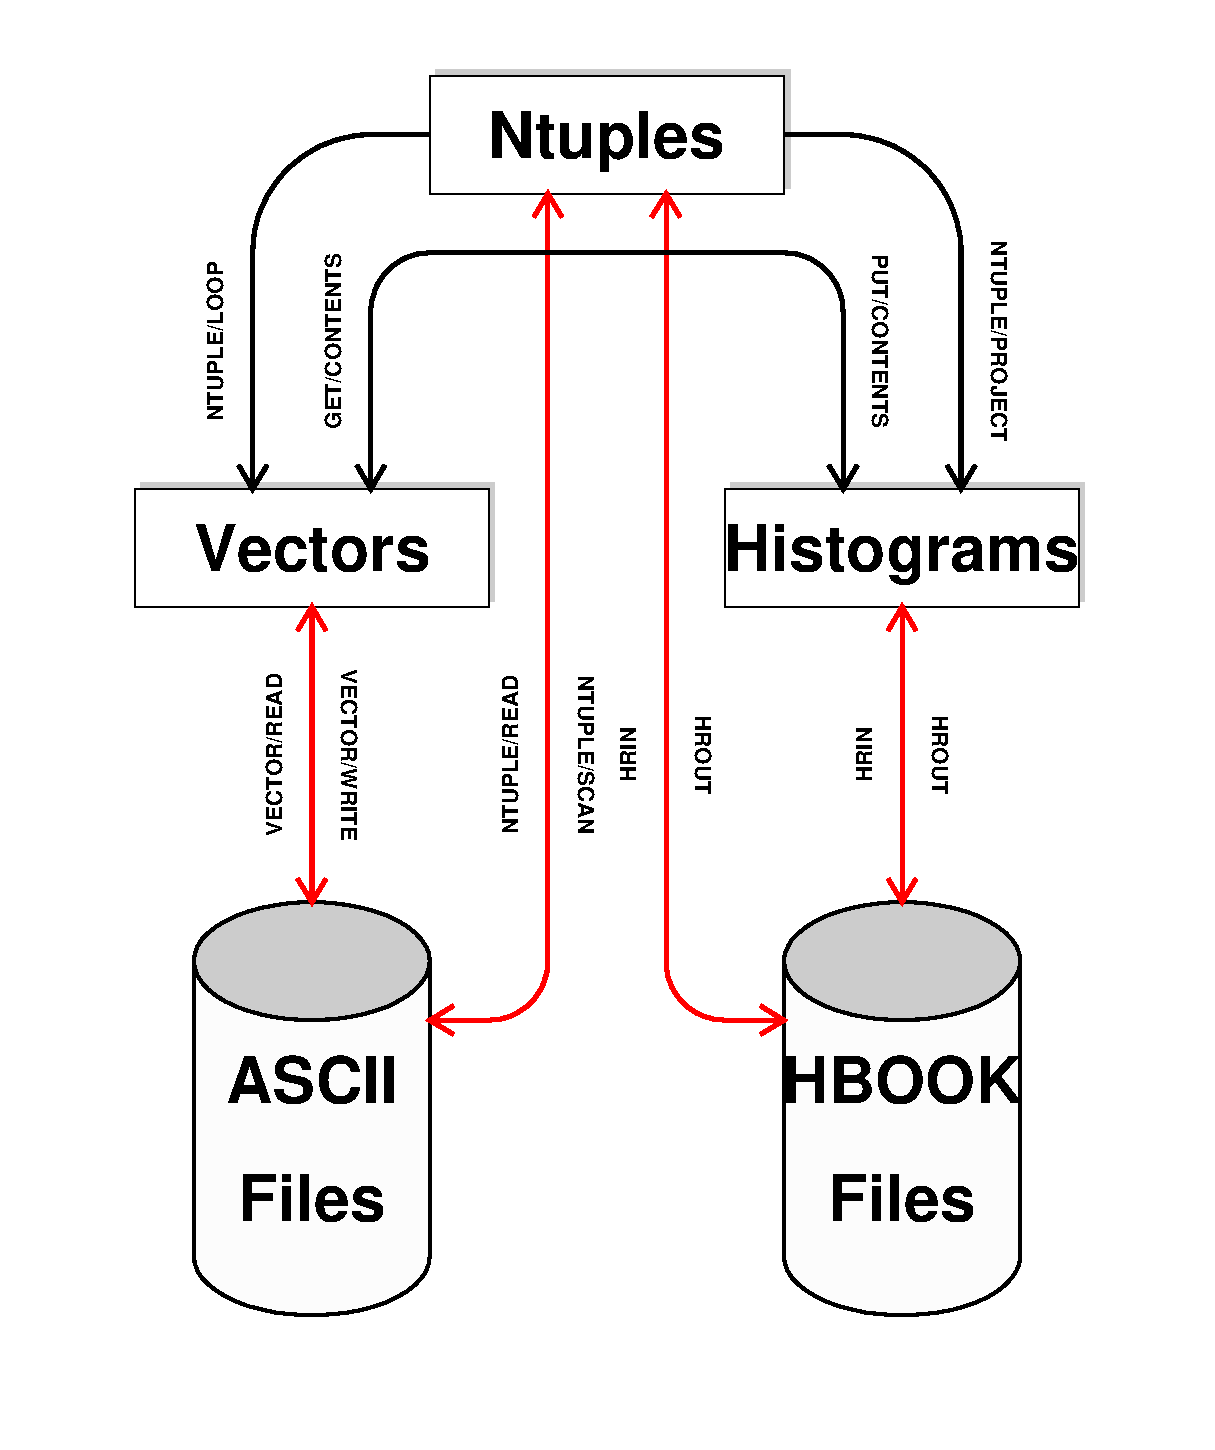
\includegraphics[width=.7\linewidth]{pawtut10.eps}
\caption{PAW entities and their related commands}
\label{fig:PAWCOM}
\end{figure}

Relations which exist between various PAW entities as described in section 
\ref{sec:pawstructure} on page~\pageref{sec:pawstructure}
and the operations which can be performed upon them have been
schematically represented in figure \ref{fig:PAWCOM}.
All commands shown in the picture next to the lines connecting the objects
have been abbreviated in a way that
they are unambiguous and can be typed to PAW, which will then
detail the various parameters to be supplied.
 
There are three main input/output formats, namely a simple text
file (e.g. with data points or commands), a direct access ZEBRA RZ file
(used by HBOOK and HIGZ for storing histograms and pictures on a given
machine) and a ZEBRA FZ sequential file, which can be used to transfer
structured ZEBRA data between various computers.
The RZ and FZ representations can be transformed into each other
using the TOALFA and FRALFA commands.
\index{ZEBRA!TOALFA}
\index{ZEBRA!FRALFA}
\index{ZEBRA!RZ file}
\index{ZEBRA!FZ file}
\index{text!data}
 
The three main PAW objects, Ntuples, histograms and vectors, can be
{\bf printed} on an alphanumeric screen (\Ucom{PRINT}
commands) or they can be plotted on a graphics screen (\Ucom{PLOT}
commands). 
The picture can be transformed into a ZEBRA data structure
and stored in a HIGZ database for later reference (e.g. editing by the
HIGZ editor), or an external presentation can be obtained via the
\index{metafile}
creation of a {\bf metafile}. 
\index{PAW!object}
\index{PRINT!commands}
\index{PLOT!commands}
\index{HIGZ}
\index{metafile}
\index{PostScript}
\index{PAW!entities}

\endinput

%\include{pawch3} Examples eliminated (only on web)
%%%% **************** Start of part 2 **************************-- >
%\mbox{}\thispagestyle{empty}\newpage
\begingroup
\newif\ifPAWman \PAWmantrue
\newif\ifKUIPman \KUIPmanfalse
\makeatletter
\input menu.sty
\makeatother
\gdef\Chap{}% initialize chapter name (for index)
\chapter{User interface - KUIP}
%\input{kuipkeywords.tex}
%%%%%%%%%%%%%%%%%%%%%%%%%%%%%%%%%%%%%%%%%%%%%%%%%%%%%%%%%%%%%%%%%%%%%%%%%%%%%%%%
%                                                                              %
%   KUIP  - Reference Manual -- LaTeX Source                                   %
%   Modified for PAW. Comes from:   Chapter 2: User Interface (KUIP manual)    %
%                                                                              %
%   Author: Alfred Nathaniel  CN/ASD                                           %
%   Editor: Michel Goossens   IT/ASD                                           %
%   Mods:   30 July 1998 Olivier Couet                                         %
%                                                                              %
%%%%%%%%%%%%%%%%%%%%%%%%%%%%%%%%%%%%%%%%%%%%%%%%%%%%%%%%%%%%%%%%%%%%%%%%%%%%%%%%

\def\PROMPT{\texttt{PAW >}}


--------------------------------------------------------------------
%
\section{Command line syntax\label{sec-command-line-syntax}}

The general syntax of a \emph{command line} is a \emph{command path}
optionally followed by an \emph{argument list}.
The command path and the arguments have to be separated from each other by one
or more space characters.
Therefore arguments containing spaces or other special characters have
to be quoted.

In the following we want to use an appropriate formalism to describe the
syntax rules.
The notation will be introduced step by step as needed.
The verbal explanation given above can be written as:

\indent\indent\begin{tabular}{rcl}
\textsl{command-line}
&\texttt{::=}&\textsl{command-path \quad \lcb\ argument \rcb}
\end{tabular}

The \textsl{slanted} symbols are non-terminal, i.e.\ they are composed
of other terminal or non-terminal symbols.  The definition of a
non-terminal symbol is denoted by ``\textbf{::=}''.  Symbols enclosed
in braces (``\texttt{\lcb...\rcb}'') are optional and they can appear
  zero or more times.

%
%---------------------------------------------------------------------------
%
\subsection{Command structure}

The set of commands is structured as an (inverted) tree as shown in
figure~\ref{FIG7}.
 
\begin{figure}[h]
\centering\includegraphics[width=.8\linewidth]{tree.eps}
\caption{Example of the PAW command tree structure}
\label{FIG7}
\end{figure}
 
This structure is comparable to a Unix file system.  The command set
can be dynamically extended by linking new commands or menus into the
tree.  Compared to a flat list structure the tree allows a cleaner
representation through menus, especially when the command set is
large.  \PAW{} has more than 200~commands.  It would be hard to
visualize such a number of command in a single graphics menu.

%
%---------------------------------------------------------------------------
%
\subsubsection{Abbreviations}

A command path consists of a menu path and a command name.
The menu path itself consists of a list of menu names up to an
arbitrarily deep level of sub-menus.

\indent\indent\begin{tabular}{rcl}
\textsl{command-path}
&\texttt{::=}&\textsl{\lsb menu-path\texttt{/\rsb}command-name} 
\\
\textsl{menu-path} 
&\texttt{::=}&
\textsl{\texttt{[/]}menu-name\texttt{\lcb/}menu-name\rcb}
\end{tabular}

Here we introduced two more notations.
Symbols in teletype mode (``\texttt{/}'') are literals, i.e.\
the menu and command names have to be separated by a slash character.
Symbols enclosed in brackets (``\texttt{[...]}'') are optional which can
appear zero or one times.

These syntax rules already show that a command path may be abbreviated by
omitting part of the leading menu path.
For example, if the complete command path is
\begin{alltt}
/MENU/SUBMENU/COMMAND
\end{alltt}
valid abbreviations are
\begin{alltt}
MENU/SUBMENU/COMMAND
SUBMENU/COMMAND
COMMAND
\end{alltt}
but \textbf{not} ``\texttt{MENU/COMMAND}'' or
``\texttt{/SUBMENU/COMMAND}''.
Note that the command name matching is case-insensitive, i.e.\ the
following are all valid possibilities:
\begin{alltt}
COMMAND
command
Command
\end{alltt}

Furthermore, menu and command names may be abbreviated by omitting
trailing parts, i.e.\
\begin{alltt}
SUB/COMMAND
COMMA
/M/S/C
\end{alltt}
are also valid abbreviations.

The shortest unambiguous abbreviation for any command is not fixed
but depends on the whole command set.
PAW lists all possible ambiguities if a given abbreviation has no
unique match:

\begin{alltt}
PAW > \underline{LIST}
 *** Ambiguous command list. Possible commands are :

 /KUIP/ALIAS/LIST
 /MACRO/LIST
 /VECTOR/LIST
 /HISTOGRAM/LIST
 /NTUPLE/LIST
 /PICTURE/LIST
\end{alltt}

\paragraph{Changing the root menu}

The command \texttt{SET/ROOT} defines the menu from which the search for
command name starts. 
It is not quite comparable to the Unix \texttt{cd} or VMS 
\texttt{SET DEFAULT} command.
If no matching command is found going downwards from the
\texttt{SET/ROOT} menu a second attempt is made starting off at the top
menu ``\texttt{/}''.

\paragraph{Disabling commands}

The command \Cind{SET/VISIBILITY} allows to disable/enable individual commands.
\index{command!visibility}
Disabled commands cannot be executed and they do not contribute to
name ambiguities.
However, the \Cind{HELP} information is still available.
Note that the \Cind{VISIBILITY} command can disable itself which makes
it impossible to re-enable any command.


\paragraph{Automatic macro execution}

The command \Cind{MACRO/DEFAULT} implements two facilities.
First it allows to define a directory search path used by the
\Cind{EXEC} command for locating \texttt{.kumac} macro files.
Second it controls the implicit interpretation of the command name token as a
possible macro filename:
\begin{DLtt}{-AutoReverse}
\item[\texttt{-Command}]
This is the default setting which does not try to interpreted
\texttt{cmd} as macro name.
\item[\texttt{-Auto}]
If the search path contains a file \texttt{cmd.kumac} it is executed,
i.e.\ the actual command becomes ``\texttt{EXEC cmd}'', otherwise the
search for a command named \texttt{cmd} starts.
\item[\texttt{-AutoReverse}]
If \texttt{cmd} is either not a command name or ambiguous and a file
\texttt{cmd.kumac} exists the command is transformed into 
``\texttt{EXEC cmd}''.
\end{DLtt}


\paragraph{Command template\label{para-set-command}}

The command \Cind{SET/COMMAND} allows to define a template which is
used whenever the command token does not match any command name.
The template can contain ``\verb!$1!'',\dots, ``\verb!$9!'' which are
substituted with the \textsl{n}'th token from the original command line,
or ``\verb!$*!'' which is replaced by the complete line.
For example, PAW can be turned into a calculator by
\begin{alltt}
\PROMPT{} \underline{SET/COMMAND 'mess $sigma($*)'}
\PROMPT{} \underline{17+2*5}
 27
\end{alltt}

``\verb!SET/COMMAND 'EXEC $*'!'' has almost the same effect as 
``\verb!DEFAULT -AutoReverse!'' but these are two distinct facilities
which can be active simultaneously.
The difference is that for \texttt{SET/COMMAND} the token in the command
name position must not match any command.
If does not apply if the token is an ambiguous command name.

Both \texttt{Auto/AutoReverse} and \texttt{SET/COMMAND} logic are ignored
during the execution of macro scripts.


%
%---------------------------------------------------------------------------
%
\subsection{Arguments}

Most commands have \emph{parameters} for which the user is expected to
supply \emph{argument values}.
Parameters are either \emph{mandatory} or \emph{optional}.
Mandatory arguments which are not specified on the command line are
prompted for.
If optional arguments are omitted a default value is used instead.

Mandatory parameters always precede the optional parameters.
The command \Cind{USAGE} allows to see the number of parameters for a command:
\begin{alltt}
\PROMPT{} \underline{usage manual}

 * KUIP/MANUAL ITEM [ OUTPUT OPTION ]
\end{alltt}
The optional parameters are enclosed in square brackets.
The default values can be seen from the help text for a command.
The \texttt{STYLE} command shown in figure~\ref{fig-help-style} 
has only optional arguments.
The corresponding default values are indicated in the help information
as ``\texttt{D=}\textsl{value}''.

\begin{figure}
\begin{alltt}
\PROMPT{} \underline{HELP STYLE}

 * KUIP/SET_SHOW/STYLE [ OPTION SGYLEN SGSIZE SGYSPA SGBORD WKTYPE ]

   OPTION     C 'Option' D='?'
   SGYLEN     R 'max Y LENgth of each menu item box' D=0.025 R=0.005:0.25
   SGSIZE     R 'space available for the application' D=0.8 R=0:0.90
   SGYSPA     R 'max Y length of space between menus' D=0.02 R=-0.5:0.50
   SGBORD     R 'X or Y border for menus' D=0.015 R=0:0.25
   WKTYPE     I 'Graphics workstation type' D=0

   Possible OPTION values are:

    ?   show current style
    C   Command line : select Command line input
    AN  Menu with Numbers : select general Alpha menu (with Numbers)
    AL  Menu with Letters : select general Alpha menu (with Letters)
\end{alltt}
\caption{Parameter types, default values, and range limits
\label{fig-help-style}}
\end{figure}

Mandatory parameters may also have a default value which is used if
the prompt is acknowledged by simple hitting the \texttt{RETURN}-key.
Otherwise the proposed default is the value used in the previous
command execution.

The \texttt{STYLE} command also shows that there are three different
kind of parameters:
character values indicated by ``\texttt{C}'' after the parameter
name, real values (``\texttt{R}'') and integer values
(``\texttt{I}'').

Numeric (real or integer) parameters may be restricted in the range of
acceptable values.
In the help text this is indicated as
``\texttt{R=\textsl{lower}:\textsl{upper}}. 
If the argument value is outside the range PAW  prompts the user to
enter an acceptable value before the command can be executed.
The lower or upper range value may be missing to indicate an unlimited
range in one direction.
Instead of a simple numeric value the argument may also be an expression.

For both numeric and character parameters the range may also be given
as a comma-separated list of values. 
PAW will accept an argument only if it matches one of
the values in the list.

In general the arguments given on the command line are assigned to the
command parameters from left to right but there are also ways to
change the order.
In our syntax notation, using ``\texttt{|}'' to indicate possible
alternatives, we can write:

\begin{tabular}{rclclclclclcl}
\textsl{argument}
&\texttt{::=}&
\textsl{value} 
&\verbar&
\texttt{!} 
&\verbar&
\texttt{!!} 
&\verbar&
\textsl{name\texttt{=}value} 
&\verbar&
\textsl{\texttt{-}value} 
\end{tabular}

An argument given as a simple value is assigned to the next parameter
expected. 
The special values ``\texttt{!}'' and ``\texttt{!!}'' are templates
for the default value and the value from the previous command
execution, respectively.

\subsubsection{Named arguments\label{sec-named-arguments}}

The form ``\textsl{name\texttt{=}value}'' allows to invert the
argument order or to skip a list of optional parameters for which
the default values should be used.
For example,
\begin{alltt}
STYLE G SGBORD=0.1
\end{alltt}
is equivalent to 
\begin{alltt}
STYLE G ! ! ! 0.1
\end{alltt}
A simple argument following a named argument is assigned to the
parameter following the named parameter, i.e.\
\begin{alltt}
STYLE G SGBORD=0.1 1
\end{alltt}
is equivalent to 
\begin{alltt}
STYLE G ! ! ! SGBORD=0.1 WKTYPE=1
\end{alltt}

Parameter names are case-insensitive but in general they may not be
abbreviated. 
In the help text the abbreviat level is indicated by a ``\texttt{*}'' inside 
the parameter name.
For example, if the parameter name is shown as
\begin{alltt}
LIB*RARY
\end{alltt}
the acceptable abbreviations are ``\texttt{LIB=}'',
``\texttt{LIBR=}'', ``\texttt{LIBRA=}'', ``\texttt{LIBRAR=}'', and
``\texttt{LIBRARY=}''.

PAW does not insist that an argument of the form
``\textsl{name\texttt{=}value}'' matches one of the parameter names. 
The argument including the ``\textsl{name\texttt{=}}'' part is simply
assigned to the next parameter expected.


\subsubsection{Option arguments}

The last alternative ``\texttt{-}\textsl{value}'' to specify an
argument applies only to \textsl{option} parameters.
(Note the distinction between \emph{option} and \emph{optional}.
Option parameters are usually but not necessarily optional.)
In the help text option parameters are tagged by the list of possible
values (figure~\ref{fig-help-manual}).
Frequently these parameters are named ``\texttt{OPTION}'' or
``\texttt{CHOPT}''. 

\begin{figure}
\begin{alltt}
PAW > \underline{HELP MANUAL}

 * KUIP/MANUAL ITEM [ OUTPUT OPTION ]

   ITEM       C 'Command or menu path'
   OUTPUT     C 'Output file name' D=' '
   OPTION     C 'Text formatting system' D=' '

   Possible OPTION values are:

   ' '     plain text : plain text format
    LATEX  LaTeX format (encapsulated)
    TEX    LaTeX format (without header)
\end{alltt}
\caption{Example for option parameters
\label{fig-help-manual}}
\end{figure}

The ``\texttt{-}\textsl{value}'' form allows to specify option
arguments out of order, emulating the Unix style of options preceded
other command arguments.
For example,
\begin{alltt}
MANUAL -LATEX /KUIP
\end{alltt}
is equivalent to 
\begin{alltt}
MANUAL /KUIP OPTION=LATEX
\end{alltt}
Note that this is \textbf{not} equivalent to 
``\texttt{MANUAL OPTION=LATEX /KUIP}''.
Unlike to the ``\texttt{-}\textsl{value}'' form subsequent simple
arguments are still assigned to the next parameter expected, not to
the one following the option parameter itself.

Since a leading ``\texttt{-}'' can be part of a valid (non-option)
argument the value is checked against a set of rules before it is
actually interpreted as an option assignment.

The option argument can be a concatenation of several of the allowed
option values.
PAW checks that the argument string is exclusively constructed from
valid option values.
This check is done by removing matches of option values from the
argument string, starting with the longest option values first.
For example, with the definition
\begin{alltt}
   Possible OPTION values are:
    AB
    ABC
    CD
\end{alltt}
the argument ``\texttt{-ABCD}'' is not interpreted as option
assignment because after removing the longest match ``\texttt{ABC}''
the remainder ``D'' is not anymore a valid option value.
(This case would have to be written as ``\texttt{-CDAB}''.

%
%---------------------------------------------------------------------------
%
\subsubsection{Argument values}

Since in command line blanks are used to separate the command name and the 
individual arguments string values containing blanks have to be quoted. The 
rules are the same as used by Fortran: the quote character is the apostrophe
``\texttt{'}'', and apostroph inside a quoted string have to be duplicated:

\begin{alltt}
MESS 'Hello world'
MESS 'Do or don''t'
\end{alltt}

Note that the \Cind{MESSAGE} command has only a single parameter:
\begin{alltt}
 * KUIP/MESSAGE [ STRING ]

   STRING     C 'Message string' D=' '
...
\end{alltt}
Nevertheless, in most cases quoting the message string is not necessary. If the 
command line contains more arguments than there are parameters the additional 
values are concatenated to the argument for the last parameter. In the 
concatenation each value is separated by a (single) blank character, i.e.\ 
the commands

\begin{alltt}
MESS 'Hello World'
MESS  Hello World
MESS  Hello       World
\end{alltt}
yield all the same output. Therefore the message text only needs quoting if the 
words should be separated by more than one space character.

Quoting inhibits the interpretation of the enclosed string as special argument
values. Printing an exclamation mark as message text has to written as

\begin{alltt}
MESS '!'
\end{alltt}

because ``\texttt{MESS !}'' would mean to take the default value for the 
parameter \Pind{STRING} and yield an empty line only.

Another instance is if an argument of the form ``\textsl{name\texttt{=}value}'' 
should be taken literally. For example, the command line

\begin{alltt}
EXEC mac foo=bar
\end{alltt}

initializes the macro variable ``\texttt{foo}'' to the value ``\texttt{bar}''. 
However, if the intention is to pass the string ``\texttt{foo=bar}'' as 
argument to the macro quotes must be used:

\begin{alltt}
EXEC mac 'foo=bar'
\end{alltt}

In addition, some commands, e.g.\

\begin{alltt}
 * NTUPLE/PLOT IDN [ UWFUNC NEVENT IFIRST NUPD OPTION IDH ]
\end{alltt}

use the form ``\textsl{name\texttt{=}value}'' for equality tests in the cut 
expression \Pind{UWFUNC}.  For example, the command

\begin{alltt}
NT/PLOT 10.energy year=1998
\end{alltt}

selects all event for which the Ntuple column \texttt{YEAR} has the value 
\texttt{1998}. Any name clash between the Ntuple column and one of the command
parameters requires quoting. If the column was called \texttt{NUPD} instead of
\texttt{YEAR} the command would have to be written as

\begin{alltt}
NT/PLOT 10.energy 'nupd=1998'
\end{alltt}

or alternatively as ``\texttt{NT/PLOT 10.energy UWFUNC=nupd=1998}''.

Finally, quoted strings are also exempted from any substitutions of aliases, 
\Key{system function}s, and \Key{macro variable}s. For example,

\begin{alltt}
MESS 'foo'
\end{alltt}
always prints ``\texttt{foo}'' while
\begin{alltt}
MESS foo
\end{alltt}

can result in ``\texttt{bar}'' if preceded by the command
``\texttt{ALIAS/CREATE foo bar}''. Since square brackets denote macro variable 
substitution and system functions names start with a dollar-sign it is 
especially recommended to quote VMS file specifications.

The operator ``\texttt{//}'' allows to concatenate several parts to a single 
argument value. Unquoted strings on either side of the concatenation operator 
are implicitly treated as literals unless they are subject to a substitution, 
i.e.\ the command lines

\begin{alltt}
MESS 'abc'//'def'
MESS 'abc'//def
MESS abc//'def'
MESS abc//def
MESS abcdef
MESS 'a'//'b'//'c'//'d'//'e'//'f'
\end{alltt}

are all equivalent (provided that \texttt{abc} and \texttt{def} are not defined 
as aliases). The character sequence ``\texttt{//}'' at the beginning or end of 
an argument is taken literally, e.g.\ in

\begin{alltt}
CD //LUN2//1
\end{alltt}

the command receives the value ``\texttt{//LUN21}''.


\subsection{More on command lines}

The command line syntax allows to write several commands in one line
and also to extend commands with long argument
lists over several lines.


\subsubsection{Multiple commands on a single line\label{sec-mult-cmd}}

An input line presented to the PAW command processor may contain
several commands separated by ``\texttt{;}''.
The commands are executed sequentially as if they were on separate
lines:
\begin{alltt}
MESS Hello world!; MESS How are you?
\end{alltt}
is equivalent to
\begin{alltt}
MESS Hello world!
MESS How are you?
\end{alltt}
Note that the text following the semicolon will not be used to satisfy
any prompts emitted by the preceding command, 
e.g.\ ``\texttt{usage; manual}'' will not behave as 
``\texttt{usage manual}''.

The semicolon is \textbf{not} interpreted as line
separator if it is immediately followed by a digit or one of the
characters
\begin{alltt}
  +  - *  ?  [
\end{alltt}
For example, issuing a VMS command with a file version number such as
\begin{alltt}
SHELL delete *.tmp;*
\end{alltt}
does not require quoting.
Note that this exception rule applies independently of the operating
system.
In order to avoid surprises we recommend to put always at least one
blank after a semicolon intended to be a line separator.

Each command execution returns a status code which is zero for success
and non-zero for failure.
The sequences ``\texttt{;\&}'' and ``\texttt{;!}'' allow to execute
the remaining part of an input line depending on the status code of
the preceding command.
With
\begin{alltt}
cmd1 ;& cmd2 ; cmd3
\end{alltt}
the commands \Cind{cmd2} and \Cind{cmd3} are only executed if
\Cind{cmd1} succeeded while with
\begin{alltt}
cmd1 ;! cmd2 ; cmd3
\end{alltt}
the remaining commands are only executed if the first one failed.
Note that the two characters must follow each other immediately
without intervening blank.

In some commands, for example \Cind{HISTO/PLOT}, one of the parameters
is marked in the help text with the attribute ``\texttt{Loop}''.
If the corresponding argument is a comma-separated list of values
PAW implicitly repeats the command for each value in the list
individually: 
\begin{alltt}
HISTO/PLOT 10,20,30
\end{alltt}
is equivalent to
\begin{alltt}
HISTO/PLOT 10
HISTO/PLOT 20
HISTO/PLOT 30
\end{alltt}
Note that ``\texttt{,}'' inside parentheses is not taken as value
separator, i.e.\
\begin{alltt}
HISTO/PLOT 10(1:25,1:25)
\end{alltt}
executes a single command.


\subsubsection{Single commands on multiple lines}

For commands with very long argument lists it can become necessary to
continue it on the next line.
An input line ending with an ``\verb!_!'' character is joined with
the following line.

In the concatenation the underscore itself and all but one of the
leading blanks from the next line are removed.
Blanks preceding the underscore are left intact.
For example,
\begin{alltt}
ME_
SS _
'Hello_
       world'
\end{alltt}
is an extravagant way of writing
\begin{alltt}
MESS 'Hello world'
\end{alltt}
Note that the interpretation of ``\verb!_!'' as line continuation
cannot be escaped.
If the command line should really end with an underscore the last
argument must be quoted.

%
%---------------------------------------------------------------------------
%
\subsubsection{Recalling previous commands}

The command lines types during a session are written into a history file.
By default the file is called \texttt{last.kumac} and is updated every
25~commands.
The commands \Cind{LAST} and \Cind{RECORDING} allow to change the file
name and the frequency.
At the start of a new session the existing file is renamed into
\texttt{last.kumacold} (except on VMS) before the new \texttt{last.kumac} is created.
Comment lines indicate the date and time at which the sessions were
started and stopped. 

\begin{table}\centering
\begin{tabular}{|l|p{.85\textwidth}|}
\hline
\texttt{{\Circ}A/{\Circ}E  } & Move cursor to beginning/end of the line. \\
\texttt{{\Circ}F/{\Circ}B  } & Move cursor forward/backward one character. \\
\texttt{{\Circ}D     } & Delete the character under the cursor. \\
\texttt{{\Circ}H, DEL} & Delete the character to the left of the cursor. \\
\texttt{{\Circ}K     } & Kill from the cursor to the end of line. \\
\texttt{{\Circ}L     } & Redraw current line. \\
\texttt{{\Circ}O     } & Toggle overwrite/insert mode. Text added in overwrite mode
               (including yanks) overwrites existing text, while insert mode
               does not overwrite. \\
\texttt{{\Circ}P/{\Circ}N  } & Move to previous/next item on history list. \\
\texttt{{\Circ}R/{\Circ}S  } & Perform incremental reverse/forward search for string on
               the history list.  Typing normal characters adds to the
               current search string and searches for a match.  Typing
               \verb!^R/^S! marks the start of a new search, and
moves on to 
               the next match.  Typing \verb!^H! or \texttt{DEL} deletes the last
               character from the search string, and searches from the
               starting location of the last search.
               Therefore, repeated \texttt{DEL}'s appear to unwind to the match
               nearest the point at which the last \verb!^R! or
\texttt{{\Circ}S} was typed. 
               If \texttt{DEL} is repeated until the search string is empty the
               search location begins from the start of the history
               list. Typing \texttt{ESC} or any other editing character accepts
               the current match and loads it into the buffer,
               terminating the search. \\
\texttt{{\Circ}T     } & Toggle the characters under and to the left of the cursor. \\
\texttt{{\Circ}U     } & Kill from the prompt to the end of line. \\
\texttt{{\Circ}Y     } & Yank previously killed text back at current location.
               Note that this will overwrite or insert, depending on
               the current mode. \\
\texttt{TAB    } & By default adds spaces to buffer to get to next \texttt{TAB} stop
               (just after every 8th column). \\
\texttt{LF, CR } & Returns current buffer to the program. \\
\hline
\end{tabular}
\caption{Key-binding for recall style {\tt KSH}
\label{tab-recall-ksh}}
\end{table}

In this way the user can keep track of all commands entered in
the previous and in the current session.
The command ``\texttt{LAST -99}'' flushes the buffered lines into
\texttt{last.kumac} and envokes the editor on the file.
The user can then extract the interactively typed commands and copy
them into another \texttt{.kumac} file from which they can be
re-executed.

The command ``\texttt{LAST -\textsl{n}}'' prints the last \textsl{n}
commands entered.
On a workstation this allows to re-execute command sequences by doing
cut-and-paste operations with the mouse.

PAW provides a mechanism similar to the one found
in the Unix \texttt{csh} shell for re-executing commands:
\begin{DLtt}{12345}
\item[\texttt{!-}\textsl{n}]
executes the \textsl{n}'th last command once more. 
\item[\texttt{!!}]
is an short-cut for ``\texttt{!-1}'' re-executing the last command.
\item[\texttt{!}\textsl{n}]
re-executes the \textsl{n}'th command entered since the beginning of the
session.
\item[\texttt{!}]
prints the commands together with their numbers.
The number of lines printed depend on the recording frequency.
\item[\texttt{!}\textsl{foo}]
re-executed the latest command line starting with the string ``\textsl{foo}''.
\end{DLtt}

The command line numbering can also be seen if the prompt string
contains ``\texttt{[]}'':
\begin{alltt}
\PROMPT{} \underline{PROMPT 'Paw[] '}
Paw[2]
\end{alltt}

On Unix and VMS PAW also provides recalling and editing of command lines
for re-executing.
The command \Cind{RECALL} allows to choose between different
key-bindings:
\begin{UL}
\item
Recall style \texttt{KSH} has an Emacs-like binding
(table~\ref{tab-recall-ksh}) similar to
the one used by the \texttt{ksh} and \texttt{bash} shells.
If the terminal returns ANSI escape sequences the arrow keys can be
used instead of \verb!^B/^F/^N/^P!. 

\item
Recall style \texttt{DCL} implements the key-binding of VMS line
editing (table~\ref{tab-recall-dcl}).

\item
The style names \texttt{KSHO} and \texttt{DCLO} allow to switch to overstrike
mode instead of the default insert mode.

\item
Recall style \texttt{NONE} directs PAW to do plain reading from the
terminal input. 
\end{UL}

\begin{table}\centering
\begin{tabular}{|l|l|}
\hline
\verb!BS/^E! & Move cursor to beginning/end of the line. \\
\verb!^F/^D! & Move cursor forward/backward one character. \\
\verb!DEL!   & Delete the character to the left of the cursor. \\
\verb!^A!    & Toggle overwrite/insert mode. \\
\verb!^B!    & Move to previous item on history list. \\
\verb!^U!    & Delete from the beginning of the line to the cursor. \\
\verb!TAB!   & Move to next \texttt{TAB} stop. \\
\verb!LF,CR! & Returns current buffer to the program. \\
\hline
\end{tabular}
\caption{Key-binding for recall style {\tt DCL}
\label{tab-recall-dcl}}
\end{table}

%
%---------------------------------------------------------------------------
%
\section{Aliases}

\Key{Alias}es allow the user to define abbreviations for parts of a
command line.
There are two types of aliases,
\emph{command aliases} and \emph{argument aliases}, which differ
in the way they are recognized in a command line.
Both alias types can be defined by the \Cind{ALIAS/CREATE} command:
\begin{alltt}
 * KUIP/ALIAS/CREATE NAME VALUE [ CHOPT ]

   NAME       C 'Alias name'
   VALUE      C 'Alias value'
   CHOPT      C 'Option' D='A'

   Possible CHOPT values are:

    A  create an Argument alias
    C  create a Command alias
    N  No alias expansion of value
\end{alltt}

The alias value may be any string but the alias name can only consist
letters, digits, ``\verb!_!'', ``\texttt{-}'', ``\texttt{@}'',
and ``\verb!$!'' characters.
Command and argument aliases share the same name space. 
If a command alias with the same name as an existing argument alias is
created, the argument alias is deleted first, and vice versa.


\subsection{Argument aliases}

If an argument alias name is recognized anywhere
in the command line it is substituted by its value.
The name matching is case-insensitive and the substitution is literally,
i.e.\ without case folding or insertion of additional blanks.
The replacement is scanned for further occurrences of alias names which
in turn will be replaced as well.

The alias name must be separated from the rest of the
command line either by a blank or by one of the special characters
\begin{alltt}
  /  ,  =  :  ;  .  %  '  (  )
\end{alltt}
(not necessarily the same character on both sides).
For example, if \texttt{foo} and \texttt{bar} are alias names,
\texttt{foot} and \texttt{Bar-B-Q} are not affected.
If two alias replacements need to be concatenated the ``\texttt{//}''
operator can be used, i.e.
\begin{alltt}
ALIAS/CREATE DIR disk$user:[paw]
ALIAS/CREATE FIL file.dat
HISTO/FILE 1 DIR//FIL
\end{alltt}
translates into ``\verb!HISTO/FILE 1 disk$user:[paw]file.dat!''.
Since argument aliases are also recognized in the command position with
the definition abbreviations like \Cind{HISTO/FIL} cannot be used anymore.

Alias substitution does not take place inside quoted strings.
The \texttt{ALIAS} commands themselves are treated as a special case.
In the command line parsing they are specifically exempted from alias
translation in order to allow aliases can be deleted and redefined
without quoting.
For example,
\begin{alltt}
\PROMPT{} \underline{ALIAS/DELETE *}
\PROMPT{} \underline{ALIAS/CREATE foo bar}
\PROMPT{} \underline{ALIAS/CREATE bar BQ}
\PROMPT{} \underline{ALIAS/CREATE foo tball}
\PROMPT{} \underline{ALIAS/LIST}
 Argument aliases:
 BAR        => BQ
 FOO        => tball
 No Command aliases defined.
\end{alltt}
redefines \texttt{FOO} rather than creating a new alias name~\texttt{BQ}.
The value part, however, is subject to alias translations.
If the aliases are created in reverse order
\begin{alltt}
\PROMPT{} \underline{ALIAS/DELETE *}
\PROMPT{} \underline{ALIAS/CREATE bar BQ}
\PROMPT{} \underline{ALIAS/CREATE foo bar}
\PROMPT{} \underline{ALIAS/LIST}
 Argument aliases:
 BAR        => BQ
 FOO        => BQ
 No Command aliases defined.
\end{alltt}
the second alias is created as ``\texttt{ALIAS/CREATE foo BQ}''.
In this case quoting the alias value does not avoid the translation.
Writing instead
\begin{alltt}
ALIAS/CREATE foo 'bar'
\end{alltt}
will yield the same result.
Since the \texttt{ALIAS} commands bypass part of the command line parsing
the translation of the value part has to be applied by the
\Cind{ALIAS/CREATE} command itself.
At that stage the information about quoting is no longer available. 

The option ``\texttt{N}'' allows to inhibit the alias expansion in the
value.
Using this option can lead to an infinite recursion of alias
translations which will be detected only when one the alias
names involved is actually used.
\begin{alltt}
\PROMPT{} \underline{ALIAS/DELETE *}
\PROMPT{} \underline{ALIAS/CREATE foo bar}
\PROMPT{} \underline{ALIAS/CREATE -N bar foo}
\PROMPT{} \underline{ALIAS/LIST}
 Argument aliases:
 BAR        => foo
 FOO        => bar
 No Command aliases defined.
\PROMPT{} \underline{foo}
 *** Recursive command alias in foo
 *** Recursive argument alias in foo
 *** Unknown command: foo
\PROMPT{} \underline{bar}
 *** Recursive command alias in bar
 *** Recursive argument alias in bar
 *** Unknown command: bar
\end{alltt}

Alias substitution happens before the command line is split-up into
command name and arguments.
Hence, aliases can represent several arguments at once.
For example,
\begin{alltt}
ALIAS/CREATE limits '100 -1.57 1.57'
FUN1 10 sin(x) limits
\end{alltt}
is equivalent to
\begin{alltt}
FUN1 10 sin(x) 100 -1.57 1.57
\end{alltt}
The quotes in the \Cind{ALIAS/CREATE} command are necessary but they are
not part of the alias value.
If an alias value containing blanks is supposed to be treated as a
single argument four extra quotes are needed in order that
\begin{alltt}
ALIAS/CREATE htitle '''X vs. Y'''
1D 10 htitle 100 0 1
\end{alltt}
is equivalent to
\begin{alltt}
1D 10 'X vs. Y' 100 0 1
\end{alltt}

Argument aliases can lead to unexpected interpretations of command lines.
For example, a user defining
\begin{alltt}
ALIAS/CREATE e EDIT
\end{alltt}
wants ``\texttt{E}'' to be short-hand for the command \Cind{EDIT}.
However, the following consequence is probably not intended:
\begin{alltt} 
PAW > \underline{nt/plot 30.e}
 ***** Unknown name ---> EDIT
\end{alltt}

For historic reasons the default option for the \Cind{ALIAS/CREATE}
command is to define an argument alias.
However, the use of argument aliases can lead to subtle side-effects and
should therefore be restricted as much as possible. 


\subsection{Command aliases}

This problem described above does not arise if a command alias is
created instead: 
\begin{alltt}
ALIAS/CREATE -C e EDIT
\end{alltt}
Command aliases are only recognized if they appear at the beginning of a
command line (ignoring leading blanks).
Hence, there is no need to protect command arguments from inadvertent
substitutions.
Furthermore the match must be exact (ignoring case differences), i.e.
the command
\begin{alltt}
/GRAPHICS/HPLOT/ERRORS
\end{alltt}
can still be abbreviated as \Cind{HPLOT/E}.

Alias values can also represent several commands by using one of the
line separators described in section~\ref{sec-mult-cmd}, e.g.
\begin{alltt}
ALIAS/CREATE -C ciao 'MESS Hello world! ; MESS How are you?'
\end{alltt}

%
%---------------------------------------------------------------------------
%
\section{System functions}\label{sec-system-functions}
\index{function|see system function}

A set of built-in, so-called \Key{system function}s 
is provided. They allow, for example, to
inquire the current dialogue style or to manipulate strings.
The complete list of available functions can be obtained from 
``\Cind{HELP KUIP/FUNCTIONS}''.

The function name is preceded by a \verb!$!-sign.
Arguments are given as a comma separated
list of values delimited by ``\texttt{(}'' and ``\texttt{)}''.
The arguments may be expressions containing other system functions.
\index{system function!arguments}

Functions without arguments must be followed by a character which is
different from a letter, a digit, an underscore, or a colon\footnote{
Excluding the colon as separator avoids the substitution of VMS
logical name containing a dollar-sign such as in 
``\texttt{DISK\$OS:[dir]file.dat!''}}.
``\verb!$OSMOSIS!'' will not be recognized as the function
``\verb!$OS!'' followed by ``\texttt{MOSIS}''.
If that is the desired effect the concatenation operator has to be used:
``\verb!$OS//MOSIS!''. 
Note however that two functions can follow each other, e.g.\
``\verb!$OS$MACHINE!'' because the \verb!$!-sign does
not belong to the function name.
\index{system function!name separators}

Depending on the setting of the \Cind{SET/DOLLAR} command
the name following the \verb!$!-sign may also be an environment
variable\footnote{%
  On VMS there is a distinction between lowercase and uppercase names.
  Uppercase names (without the \texttt{\$}-sign) are searched for
  first in the logical name tables and then in the symbol table while
  lowercase names are searched for only in the symbol table.  The
  names \texttt{HOME}, \texttt{PATH}, \texttt{TERM}, and \texttt{USER}
  have a predefined meaning.  In order to avoid conflicts with DCL
  symbols which are merely defined as abbreviations for running
  executables and DCL procedures all values starting with a
  ``\texttt{\$}'' or ``\texttt{@}'' character are excluded from
  substitution.}.  
The replacement value for ``\verb!$!\textsl{xxx}'' is obtained 
in the following order:
\begin{OL}
\item
If \textsl{xxx} is a system function followed by the correct
number and types of arguments, replace it by its value.
\item
Otherwise if \textsl{xxx} is an argument-less system functions, replace it by
its value.
\item
Otherwise if \textsl{xxx} is a defined environment variable, replace it
by its value.
\item
Otherwise no replacement takes place.
\end{OL}


\subsection{Inquiry functions}


\subsubsection{Style inquiries}

\begin{UL}

\item\SysFdef{STYLE}{}\label{ref-dollar-style}
returns the name of the currently active dialogue
style (``\texttt{C}'', ``\texttt{G}'', ``\texttt{GP}'', etc.).
This allows, for example, to a common logon macro containing different
default setups depending whether PAW is started in command
line mode or in \Motif{} mode:
\begin{alltt}
IF $STYLE='XM' THEN
   ...
ELSE
   ...
ENDIF
\end{alltt}

\item\SysFdef{LAST}{}
returns the previously executed command sequence:
\begin{alltt}
\PROMPT{} \underline{MESS Hello world! ; MESS How are you?}
 Hello world!
 How are you?
\PROMPT{} \underline{MESS $LAST}
 MESS Hello world! ; MESS How are you?
\end{alltt}

\item\SysFdef{KEYVAL}{}
returns the content of the last selected panel box in
style~\texttt{GP} and 
\item\SysFdef{KEYNUM}{} returns row/column address in
the form ``\textsl{row\texttt{.}col}''.
The column address is always given as a two-digit number.
\end{UL}

\subsubsection{Alias inquiries}

\begin{UL}

\item\SysFdef{ANUM}{}
returns the number of \emph{argument} aliases
currently defined. 

\item\SysFdef{ANAM}{n}
returns the name and
\item\SysFdef{AVAL}{n} returns the value of the \textsl{n}'th
argument alias.
No substitution takes place if \textsl{n} is not a number between 1
and \verb!$ANUM!.
There is no guarantee that ``\verb!$ANAM($ANUM)!'' refers to the
most recently created alias.

\end{UL}

\subsubsection{Vector inquiries}

\begin{UL}

\item
\SysFdef{NUMVEC}{} returns the number of vectors currently defined.

\item
\SysFdef{VEXIST}{name} returns a positive number if a vector
\textsl{name} is currently defined.
The actual value returned is undefined and may even change between
tests on the same \textsl{name}.
If the vector is undefined the value ``\texttt{0}'' is returned.

\item
\SysFdef{VDIM}{name,dim} returns the vector
size along index dimension \textsl{dim};
\(dim=1\) is used if the second argument is omitted.
If the vector is undefined the value ``\texttt{0}'' is returned.

\item
\SysFdef{VLEN}{name} returns for a 1-dimensional vector the index of the last non-zero element. 
For 2- and 3-dimensional vectors the result is the same as for \SysFind{VDIM}.
If the vector is undefined the value ``\texttt{0}'' is returned.

\end{UL}

\begin{alltt}
PAW > \underline{V/CREATE v1(10) R 1 2 3 4 0 6}
PAW > \underline{MESS $VDIM(v1) $VLEN(v1)}
 10 6 
PAW > \underline{V/CREATE v2($VLEN(v1))}
PAW > \underline{MESS $VDIM(v2) $VLEN(v2)}
 6 0 
\end{alltt}

\subsubsection{Environment inquiries}

\begin{UL}
\item\label{ref-dollar-args}
\SysFdef{ARGS}{} returns the program arguments with which PAW
was invoked. 
\item
\SysFdef{DATE}{} returns the current date in the format
``\textsl{dd}\texttt{/}\textsl{mm}\texttt{/}\textsl{yy}''.
\item
\SysFdef{TIME}{} returns the current time in the format
``\textsl{hh}\texttt{/}\textsl{mm}\texttt{/}\textsl{ss}''.
\item
\SysFdef{RTIME}{} returns the number of seconds elapsed since the
previous usage of \SysFind{RTIME}.
\item
\SysFdef{CPTIME}{} returns the seconds of CPU time spent since the
previous usage of \SysFind{CPTIME}.
\item
\SysFdef{OS}{} returns an identification for the operating system PAW is
running on, e.g.\ ``\texttt{UNIX}'', ``\texttt{VMS}'' etc...
\item
\SysFdef{MACHINE}{} returns an identification for the particular hardware
platform or Unix brand, e.g.\ ``\texttt{HPUX}'', ``\texttt{IBM}'', or
``\texttt{VAX}''.
Table~\ref{tab-os-machine} shows the \SysFind{OS} and
\SysFind{MACHINE} values for the different platforms.

On Unix platforms the operating system version can be obtained by
\SysFind{SHELL}\texttt{('uname -r')}.
\item
\SysFdef{PID}{} returns the process number or ``\texttt{1}'' if
the operating system does not support the notion of process IDs.
\item
\SysFdef{IQUEST}{i} returns the \textsl{i}'th component of the
status vector
\index{IQUEST@\texttt{IQUEST}|Sidef}
\index{QUEST@\texttt{QUEST}|see{\texttt{IQUEST}}}
\begin{alltt}
      COMMON /QUEST/ IQUEST(100)
\end{alltt}
\Rind{IQUEST(1)} always contains the return code of the most recently
executed command.
\item
\SysFdef{DEFINED}{name} returns \textsl{name} if a variable of that
name is defined, or the empty string if the variable is not defined.
The argument can contain ``\texttt{*}'' as wildcard matching any sequence
of characters.
All matching variable names are returned as a blank separated list.
\item
\SysFdef{ENV}{name} returns the value of the environment
variable \textsl{name}, or the empty string if the variable is not defined.
\item
\SysFdef{FEXIST}{filename} returns ``\texttt{1}'' if the file
exists, or ``\texttt{0} otherwise.
\item
\SysFdef{SHELL}{command,n} returns the \textsl{n}'th line
of output from the shell command.
\item
\SysFind{SHELL}{(\textsl{command,sep})} returns the output from the 
shell command, where newlines are replaced by the separator string.
The \textsl{sep} argument can be omitted and defaults to a single
blank character.  

The \SysFind{SHELL} function is operational only on Unix systems.
The \textsl{command} string is passed to the shell set by the
\Cind{HOST\_SHELL} command.
Alias definitions etc.\ in the shell specific startup script (e.g.\
\texttt{.cshrc}) are taken into account.
\end{UL}

\begin{table}
\centering\begin{tabular}{|l||l|l|}
\hline
\SysFind{OS} & \SysFind{MACHINE} & Platform \\
\hline
{\tt UNIX} & {\tt ALPHA} & DEC Alpha OSF \\
{\tt UNIX} & {\tt APOLLO} & HP/Apollo DomainOS \\
{\tt UNIX} & {\tt CONVEX} & Convex \\
{\tt UNIX} & {\tt CRAY} & Cray Unicos \\
{\tt UNIX} & {\tt DECS} & DECstation Ultrix \\
{\tt UNIX} & {\tt HPUX} & HP/UX \\
{\tt UNIX} & {\tt IBMAIX} & AIX for IBM/370 \\
{\tt UNIX} & {\tt IBMRT} & AIX for RS/6000 \\
{\tt UNIX} & {\tt LINUX} & Linux for PCs \\
{\tt UNIX} & {\tt NEXT} & NeXT \\
{\tt UNIX} & {\tt SGI} & Silicon Graphics Irix \\
{\tt UNIX} & {\tt SOLARIS} & Sun Solaris \\
{\tt UNIX} & {\tt SUN} & SunOS \\
{\tt VM} & {\tt IBM} & VM/CMS for IBM/370 \\
{\tt MVS} & {\tt IBMMVS} & MVS for IBM/370 \\
{\tt VMS} & {\tt ALPHA} & VMS for Alpha \\
{\tt VMS} & {\tt VAX} & VMS for Vax \\
{\tt MSDOS} & {\tt IBMPC} & MSDOS for PCs \\
{\tt WINNT} & {\tt ALPHA} & Windows/NT for DEC Alpha \\
{\tt WINNT} & {\tt IBMPC} & Windows/NT for PCs \\
\hline
\end{tabular}
\caption{Platform identification with {\tt \$OS} and {\tt \$MACHINE}}
\label{tab-os-machine}
\end{table}


\subsection{String manipulations}

\begin{UL}

\item
\SysFdef{LEN}{string} returns the number of characters in
\textsl{string}.

\item
\SysFdef{INDEX}{string,substring} returns the position
of the first occurence of \textsl{substring} inside \textsl{string} or
zero if there is none.

\item
\SysFdef{LOWER}{string} and

\item
\SysFdef{UPPER}{string} return the argument $string$
converted to lower or upper case, respectively.
\item
\SysFdef{SUBSTRING}{string,k,n} returns
the substring
\begin{ULc}
\item
$string(k:k+n-1)$ if $k>0$, or
\item
$string(l+k+1:l+k+n)$ 
if $k\le0$, where $l=\mathtt{LEN}(string)$.
\end{ULc}
In any case the upper bound is clamped to $\mathtt{LEN}(string)$.  The
argument $n$ may be omitted and the result will extend to the end of
$string$.  Character counting starts with 1; by definition the
replacement is empty if $k=0$ or $n=0$.  If $n<0$ an error
message is emitted.
\begin{alltt}
\PROMPT{} \underline{MESS $SUBSTRING(abcde,2)/$SUBSTRING(abcde,2,3)}
 bcde/bcd
\PROMPT{} \underline{MESS $SUBSTRING(abcde,-2)/$SUBSTRING(abcde,-4,3)}
 de/bcd
\end{alltt}

\item
\SysFdef{WORDS}{string,sep} returns the number of
words in \textsl{string} separated by the \textsl{sep} character.
Leading and trailing separators are ignored and strings of consecutive
separators count as one only.
The second argument may be omitted and defaults to blank as the
separator character.
\begin{alltt}
\PROMPT{} \underline{MESS $WORDS(',abc,def,,ghi',',')}
 3
\end{alltt}

\item
\SysFdef{WORD}{string,k,n,sep}
returns \textsl{n} words starting from word \textsl{k}.
The last two arguments may be omitted default to blank as separator character
and the replacement value extending to the last word in \textsl{string}.
\begin{alltt}
\PROMPT{} \underline{MESS $WORD('abc def ghi',2)}
 def ghi
\PROMPT{} \underline{MESS $WORD('abc def ghi',2,1)}
 def
\end{alltt}

\item
\SysFdef{QUOTE}{string} returns a quoted version of
\textsl{string}, i.e.\ the string is enclosed by quote characters and
quote characters inside \textsl{string} are duplicated.
The main use of this function is if an alias value containing blanks
should be treated as a single lexical token in a command line:
\begin{alltt}
ALIAS/CREATE htitle 'Histogram title'
1d 10 $QUOTE(htitle) 100 0 1
\end{alltt}
Another useful application of \SysFind{QUOTE} is to pass the value of an
alias or macro variable as a character constant to a \COMIS{} function,
for example
\begin{alltt}
foo = 'bar'
CALL fun.f($QUOTE([foo]))
\end{alltt}
is equivalent to ``\texttt{CALL fun.f('bar')}''.
Since the quotes around ``\texttt{'bar'}'' are not part of the variable
value the construct ``\texttt{CALL fun.f([foo])}'' would given the
desired result only if the value contains blanks forcing the implicit
quoting in the variable substitution.

\item
\SysFdef{UNQUOTE}{string} returns a \textsl{string} with
enclosing quote characters removed.
The main use of this function is if a macro variable should be treated
as several blank-separated lexical tokens:
\begin{alltt}
limits = '100 0 1'
1d 10 'Histogram title' $UNQUOTE([limits])
\end{alltt}
\end{UL}


\subsection{Expression evaluations}

\begin{UL}

\item
\SysFdef{EXEC}{cmd} executes a macro command and returns the
macro's \Cind{EXITM} value.
Thus
\begin{alltt}
mess $EXEC('mname 5')
\end{alltt}
is equivalent to
\begin{alltt}
EXEC mname 5
mess [@]
\end{alltt}

\item
\SysFdef{EVAL}{expr} returns the value of a numeric
expression.
The expression can contain numeric constants and references to vector
elements joined by 
``\texttt{+}'', \texttt{-}'', ``\texttt{*}'', ``\texttt{/}''.
Parentheses may be used to override the usual operator precedence.
In addition, the functions 
\texttt{ABS(\textsl{x})} (absolute value),
\texttt{INT(\textsl{x})} (truncation towards zero), and 
\texttt{MOD(\textsl{x},\textsl{y})} (modulus) are available.
Note that all operations, including division of two integer numbers, use
floating point arithmetic.
\begin{alltt}
\PROMPT{} \underline{V/CREATE vec(3) R 1.2 3.4 4.5}
\PROMPT{} \underline{MESS $EVAL((2+3)/4) $EVAL(vec(1)+vec(2)+vec(3))}
 1.25 9.1
\end{alltt}
Even if \textsl{expr} is merely a constant,
the result is always in a canonical format with a maximum of 6~non-zero
digits. 
Non-significant zeroes and the decimal point are omitted
after rounding the last digit towards \(+\infty\) or \(-\infty\).
A mantissa/exponent notation is used if the absolute value is 
\(\ge10^6\) or \(<10^{-4}\).
\begin{alltt}
\PROMPT{} \underline{MESS $EVAL(1.500) $EVAL(14.99999) $EVAL(0.000015)}
 1.5 15 1.5E-05
\end{alltt}
The explicit use of \SysFind{EVAL} is only necessary if the result
should be inserted in a place where a string is expected, for example in
the \Cind{MESSAGE} command.
In the instances where a command expects an integer or real argument
expressions are implicitly evaluated even without the \SysFind{EVAL}
function.

\item\label{ref-sigma-function}
\SysFdef{SIGMA}{expr} passes the expression to \SIGMA{} for
evaluation.
\SIGMA{} is an array manipulation package which supports a multitude of
mathematical functions (\texttt{SQRT}, \texttt{EXP}, etc.) operating on
scalars and vectors:
\begin{alltt}
PAW > \underline{V/CREATE v10(10) R 1 2 3 4 5 6 7 8 9 10}
PAW > \underline{MESS $SIGMA(2*pi) $SIGMA(vsum(v10))}
 6.28319 55
\end{alltt}
For a description of the complete \SIGMA{} expression syntax refer to
chapter~\ref{chap-sigma}.

\SIGMA{} expressions do not follow the syntax rules for PAW
expressions.
Therefore they cannot contain PAW system functions with arguments.
They may, however, contain argument-less system functions, alias names,
and macro variables.

\item
\SysFdef{RSIGMA}{} is a slight variation of \SysFind{SIGMA}.
Both functions return a scalar result in the same canonical format
used by \SysFind{EVAL}.
The only difference is that \SysFind{SIGMA} removes the decimal point
from integral values while \SysFind{RSIGMA} leaves it in.
For example, \SysFind{RSIGMA} should be used to calculate argument
values to be passed to a \COMIS{} routine 

\begin{alltt}
      SUBROUTINE FUN(X)
      PRINT *,X
      END
\end{alltt}
as floating point constants:
\begin{alltt}
PAW > \underline{CALL fun.f($SIGMA(sqrt(8)))}
  2.828430    
PAW > \underline{CALL fun.f($SIGMA(sqrt(9)))}
  .4203895E-44
PAW > \underline{CALL fun.f($RSIGMA(sqrt(9)))}
  3.000000
\end{alltt}

\end{UL}

If the expression evaluates to a vector result \SysFind{SIGMA} (and
\SysFind{RSIGMA}) return the name of a temporary vector containing
the result.
\SysFind{SIGMA} with a vector result can be used in all places where a
vector name is expected, e.g.\
\begin{alltt}
PAW > \underline{V/PRINT $SIGMA(sqrt(array(3,1#3)))}
 ?SIG1(1) = 1
 ?SIG1(2) = 1.41421
 ?SIG1(3) = 1.73205
\end{alltt}
The lifetime of these vectors is limited to the current command.
Hence, their names should not be assigned to macro variables and not be
used in alias definitions: 
\begin{alltt}
PAW > \underline{A/CREATE square_roots $SIGMA(sqrt(array(3,1#3)))}
PAW > \underline{V/PRINT square_roots}
 *** VECTOR/PRINT: unknown vector ?SIG1
\end{alltt}

\begin{UL}

\item
\SysFdef{FORMAT}{expr,format} returns the expression
value formatted according to the Fortran \textsl{format} specifier.
The possible formats are ``\texttt{F}'', ``\texttt{E}'', ``\texttt{G}'',
``\texttt{I}'', and ``\texttt{Z}'' (hexadecimal).
\begin{alltt}
\PROMPT{} \underline{MESS 'x = '//$FORMAT(1.5,F5.2)}
 x =  1.50
\PROMPT{} \underline{MESS 'i = '//$FORMAT(15,I5)}
 i =    15
\PROMPT{} \underline{MESS 'j = '//$FORMAT(15,I5.4)}
 j =  0015
\end{alltt}

\item
\SysFdef{INLINE}{name} allows to insert the value of an alias
or macro variable into an expression which is then treated as being part
of the expression.
For example,
\begin{alltt}
convert = '$UPPER'
foo = $INLINE([convert])('bar')
\end{alltt}
is equivalent to ``\verb!foo = $UPPER('bar')!'',
i.e.\ ``\texttt{foo = 'BAR'}''.
Without \SysFind{INLINE} the content of \texttt{[convert]} would be
treated as a text string with the result that 
``\verb!foo = '$UPPER(''bar'')'!''.

\end{UL}

%%%%%%%%%%%%%%%%%%%%%%%%%%%%%%%%%%%%%%%%%%%%%%%%%%%%%%%%%%%%%%%%%%%%%%%%%%%%%%%%
%                                                                              %
%   PAW   - Reference Manual -- LaTeX Source                                   %
%                                                                              %
%   PAW system functions (used by kuipch2.tex)                                 %
%                                                                              %
%   Editor: Michel Goossens / CN-AS                                            %
%   Last Mod.: 6 October 1993 oc                                               %
%                                                                              %
%%%%%%%%%%%%%%%%%%%%%%%%%%%%%%%%%%%%%%%%%%%%%%%%%%%%%%%%%%%%%%%%%%%%%%%%%%%%%%%%
\subsection{Histograms inquiry functions}
\begin{UL}
\item\texttt{\$HEXIST(id)} returns 1 if histogram \texttt{id} exists or 0 otherwise
\item\texttt{\$HINFO(id,'ENTRIES')} returns the number of entries.
\item\texttt{\$HINFO(id,'MEAN')} returns the mean value.
\item\texttt{\$HINFO(id,'RMS')} returns the standard deviation.
\item\texttt{\$HINFO(id,'EVENTS')} returns the number of equivalent event.
\item\texttt{\$HINFO(id,'OVERFLOW')} returns the content of overflow channel.
\item\texttt{\$HINFO(id,'UNDERFLOW')} returns the content of underflow channel.
\item\texttt{\$HINFO(id,'MIN')} returns the minimum bin content.
\item\texttt{\$HINFO(id,'MAX')} returns the maximum bin content.
\item\texttt{\$HINFO(id,'SUM')} returns the total histogram content.
\item\texttt{\$HINFO(id,'XBINS')} returns the number of bins in X direction.
\item\texttt{\$HINFO(id,'XMIN')} returns the lower histogram limit in X direction.
\item\texttt{\$HINFO(id,'XMAX')} returns the upper histogram limit in X direction.
\item\texttt{\$HINFO(id,'YBINS')} returns the number of bins in Y direction.
\item\texttt{\$HINFO(id,'YMIN')} returns the lower histogram limit in Y direction.
\item\texttt{\$HINFO(id,'YMAX')} returns the upper histogram limit in Y direction.
\item\texttt{\$HTITLE(id)} returns the histogram title.
\end{UL}

\subsection{Graphics inquiry functions}
\begin{UL}
\item\texttt{\$GRAFINFO('XZONES')} returns the number of zones in X direction.
\item\texttt{\$GRAFINFO('YZONES')} returns the number of zones in Y direction.
\item\texttt{\$GRAFINFO('NT')} 
returns the current normalization transformation number.
\item\texttt{\$GRAFINFO('WNXMIN')} 
returns the lower X limit of window in current NT.
\item\texttt{\$GRAFINFO('WNXMAX')} 
returns the upper X limit of window in current NT.
\item\texttt{\$GRAFINFO('WNYMIN')} 
returns the lower Y limit of window in current NT.
\item\texttt{\$GRAFINFO('WNYMAX')} 
returns the upper Y limit of window in current NT.
\item\texttt{\$GRAFINFO('VPXMIN')} 
returns the lower X limit of viewport in current NT.
\item\texttt{\$GRAFINFO('VPXMAX')} 
returns the upper X limit of viewport in current NT.
\item\texttt{\$GRAFINFO('VPYMIN')} 
returns the lower Y limit of viewport in current NT.
\item\texttt{\$GRAFINFO('VPYMAX')} 
returns the upper Y limit of viewport in current NT.
\item\texttt{\$GRAFINFO('?attr')} returns the current value of the \HPLOT/\HIGZ{}
                              attribute \texttt{attr}. See the HELP of the command
                              \texttt{SET} to have the list of the valid values of
                              \texttt{attr}.
\end{UL}

\subsection{Cuts manipulations}
\begin{UL}
\item\texttt{\$CUT(n)} returns the cut expression \texttt{\$n}
\item\texttt{\$CUTEXPAND(string)} 
replace \texttt{\$n} in the (quoted) string by \texttt{\$CUT(n)}
\end{UL}



%
%---------------------------------------------------------------------------
%

\section{Vectors}

PAW provides the facilities to store vectors of integer or real data.
These vectors, or rather arrays with up to 3~index dimensions, can be
manipulated by PAW commands (see ``\texttt{HELP VECTOR}'').
Furthermore they are interfaced to the array manipulation package
\SIGMA{} and to the Fortran interpreter \COMIS{}
(see chapter \ref{chap-sigma}).

Vectors are memory resident only, i.e.\ they are not preserved across
program executions.
The commands \Cind{VECTOR/READ} and \Cind{VECTOR/WRITE} allow to save and
restore vector data from an external file in text format.

Vector names may be composed of letters, digits, underscores and
question marks up to a maximum length of 32~characters\footnote{
Vector names which should be processed by \SIGMA{} are currently
limited to 7~characters.
}.
Names starting with ``\texttt{?}'' are reserved for internal use by
PAW.

The only exception is the predefined vector simply called ``\texttt{?}''
which has a fixed size of 100~real elements.
Unlike the others the ``\texttt{?}'' vector is mapped to a fixed memory
location (the common block \texttt{/KCWORK/}).
It does not show up in \Cind{VECTOR/LIST} output and it is not counted
in the result of \SysFind{NUMVEC}.


\begin{figure}
Definition: \Command{VECTOR/CREATE V(NCOL)}
\begin{alltt} 
+---+---+---+---+
|   |   | * |   |   * {\rm is addressed by} V(3)
+---+---+---+---+
\end{alltt} 

Definition: \Command{VECTOR/CREATE V(NCOL,NROW)}
\begin{alltt} 
+---+---+---+---+               V(:,3) {\rm is the 1-dim array representing the 3rd row}
|   |   |   |   |               V(2,:) {\rm is the 1-dim array representing the 2nd column}
+---+---+---+---+                      {\rm the shortcut notation \texttt{V(2)} can be used as well}
|   |   |   |   |
+---+---+---+---+
|   | * |   |   |   * {\rm is addressed by} V(2,3)
+---+---+---+---+
\end{alltt} 

Definition: \Command{VECTOR/CREATE V(NCOL,NROW,NPLANE)}
\begin{alltt} 
    +---+---+---+---+
  +---+---+---+---+ |
+---+---+---+---+ |-+
|   |   | * |   |-+ |   * {\rm is addressed by} V(3,1,1)
+---+---+---+---+ |-+
|   |   |   |   |-+ |
+---+---+---+---+ |-+
|   |   |   |   |-+
+---+---+---+---+  
\end{alltt}
\caption{Addressing scheme for vectors
\label{fig-vector-addressing}}
\end{figure}

\subsection{Creating vectors}

Vectors can be created with the \Cind{VECTOR/CREATE} command.
The size of the index dimensions is given in Fortran notation, e.g.\
\begin{alltt}
VECTOR/CREATE v1(100)
VECTOR/CREATE v2(10,10)
\end{alltt}
The lower index bound always starts off at~1, i.e.\ 
``\texttt{V/CREATE v(-10:10)}'' is not allowed.
Omitting the index dimension as in
\begin{alltt}
VECTOR/CREATE v
\end{alltt}
is equivalent to
\begin{alltt}
VECTOR/CREATE v(1)
\end{alltt}

PAW does not keep track of the actual number of index dimension given in
the \Cind{VECTOR/CREATE} command, i.e.\
\begin{alltt}
VECTOR/CREATE v1(10)
VECTOR/CREATE v3(10,1,1)
\end{alltt}
are equivalent.


\subsection{Accessing vectors}

Single vector elements can be used in expressions where they are treated as 
numeric constants. Vectors with a single element only we will refer to as 
``\emph{scalar vectors}''. They have the special property that in expressions 
it is sufficient to give the name without the ``\texttt{(1)}'' subscript.

Complete vectors and vector subranges can be used in the \SysFind{SIGMA} 
function and as argument to commands expecting a vector name. The subrange 
notation is the same as in Fortran, e.g.\ \texttt{v(3:5)}. The elements of 
arrays are stored in column-major order, i.e.\ the elements \texttt{v(1,2)} 
and \texttt{v(2,2)} are adjacent in memory (see 
figure~\ref{fig-vector-addressing}).

The vector processing commands are expected to deal only with contiguous 
vectors. Therefore a subrange referring to a non-contiguous set of elements is
copied into a temporary vector and cannot be used as output parameter.


%---------------------------------------------------------------------------
\section{Expressions\label{sec-expressions}}

PAW has a built-in parser for different kinds of expressions:
arithmetic expressions, boolean expressions, string expressions, and
``garbage expressions''.

\begin{table}
\hrule
\begin{tabular}{rclp{.44\textwidth}}
\textsl{expr}
&\texttt{::=}& 
\textsl{number} \\
&\verbar&  
\textsl{vector-name}
  & for scalar vectors \\
&\verbar&  
\textsl{vector-name} \texttt{(} \textsl{expr} \texttt{)} \\
&\verbar&  
\textsl{vector-name} \texttt{(} \textsl{expr}
                     \texttt{,} \textsl{expr} \texttt{)} \\
&\verbar&  
\textsl{vector-name} \texttt{(} \textsl{expr}
                     \texttt{,} \textsl{expr}
                     \texttt{,} \textsl{expr} \texttt{)} \\
&\verbar&
\texttt{[}\textsl{variable-name}\texttt{]}
  & if variable value has form of a numeric constant
    or is the name of a scalar vector \\
&\verbar&  
\texttt{[}\textsl{variable-name}\texttt{]} \texttt{(} \textsl{expr} ... \texttt{)}
  & if variable value is a vector name \\
&\verbar&  
\textsl{alias-name}
  & if alias value has form of a numeric constant \\
&\verbar&  
\verb!$!\textsl{system-function} \texttt{(...)}
  & if function returns a numeric value \\
&\verbar&
\texttt{-} \textsl{expr} \\
&\verbar&  
\textsl{expr} \texttt{+} \textsl{expr} \\
&\verbar&  
\textsl{expr} \texttt{-} \textsl{expr} \\
&\verbar&  
\textsl{expr} \texttt{*} \textsl{expr} \\
&\verbar&  
\textsl{expr} \texttt{/} \textsl{expr} \\
&\verbar&  
\texttt{(} \textsl{expr} \texttt{)} \\
&\verbar&  
\texttt{ABS (} \textsl{expr} \texttt{)} \\
&\verbar&  
\texttt{INT (} \textsl{expr} \texttt{)} \\
&\verbar&  
\texttt{MOD (} \textsl{expr} \texttt{,} \textsl{expr} \texttt{)} \\
\end{tabular}
\caption{Syntax for arithmetic expressions}
\label{tab-expr-syntax}
\hrule
\end{table}

\subsection{Arithmetic expressions\label{sec-arith-expr}}

The syntactic elements for building arithmetic expressions are shown
in table~\ref{tab-expr-syntax}.
They can be used
\begin{ULc}
\item
in the macro statements \texttt{DO}, \texttt{FOR}, and \texttt{EXITM};
\item 
in macro variable assignments;
\item
as system function arguments where a numeric value is expected;
\item
as argument to the \SysFind{EVAL} function.
\end{ULc}

Note that all arithmetic operations are done in floating point, i.e.\
``\texttt{5/2}'' becomes ``\texttt{2.5}''.
If a floating point result appears in a place where an integer is
expected, for example as an index, the value is truncated.


\subsection{Boolean expressions}

Boolean expressions can only be used in the macro statements
\texttt{IF}, \texttt{WHILE}, and \texttt{REPEAT}.
The possible syntactic elements are shown in table~\ref{tab-bool-syntax}.

\begin{table}
\hrule
\begin{tabular}{p{.5\textwidth}p{.4\textwidth}}
\begin{tabular}{rcl}
\textsl{bool} 
&\texttt{::=}& 
\textsl{expr rel-op expr} \\
&\verbar&  
\textsl{string eq-op string} \\
&\verbar&  
\textsl{expr eq-op string} \\
&\verbar&  
\texttt{.NOT.} \textsl{bool} \\
&\verbar&  
\textsl{bool} \texttt{.AND.} \textsl{bool} \\
&\verbar&  
\textsl{bool} \texttt{.OR.} \textsl{bool} \\
&\verbar&  
\texttt{(} \textsl{bool} \texttt{)} \\
\end{tabular} &
\begin{tabular}{rcccccccc}
\textsl{rel-op} 
&\texttt{::=}&
\texttt{.LT.} 
&\verbar& 
\texttt{.LE.} \\
&\verbar&  
\texttt{<} 
&\verbar& 
\texttt{<=} \\
&\verbar& 
\texttt{.GT.}
&\verbar& 
\texttt{.GE.} \\ 
&\verbar& 
\texttt{>} 
&\verbar& 
\texttt{>=} \\
&\verbar& 
\textsl{eq-op} \\
\textsl{eq-op} 
&\texttt{::=}& 
\texttt{.EQ.} 
&\verbar& 
\texttt{.NE.} \\
&\verbar&  
\texttt{=}  
&\verbar&  
\texttt{<>}  \\
\end{tabular}
\end{tabular}
\caption{Syntax for boolean expressions}
\label{tab-bool-syntax}
\hrule
\end{table}

In addition, a single arithmetic expression is also accepted as 
boolean expression, interpreting any non-zero value as \textsl{true}.
This allows, for example, the short-cuts
\begin{alltt}
IF $VEXIST(v1) THEN
...
WHILE 1 DO
...
\end{alltt}
instead of the explicit forms
\begin{alltt}
IF $VEXIST(v1)<>0 THEN
...
WHILE 1=1 DO
...
\end{alltt}

Note, however, that an arithmetic expression is \textbf{not} equivalent to a
boolean value.
This implies that
\begin{alltt}
IF $VEXIST(v1) .and. $VEXIST(v2) THEN   | error
\end{alltt}
is not accepted and has to be written as
\begin{alltt}
IF $VEXIST(v1)<>0 .and. $VEXIST(v2)<>0 THEN
\end{alltt}


\begin{table}
\hrule
\begin{tabular}{rcll}
\textsl{string}
&\texttt{::=}&  
\textsl{quoted-string} \\
&\verbar&  
\textsl{unquoted-string} \\
&\verbar&  
\textsl{string} \texttt{//} \textsl{string}
   & concatenation \\
&\verbar&  
\textsl{expr} \texttt{//} \textsl{string}
   & value of expression converted to string representation \\
&\verbar&  
\texttt{[}\textsl{variable-name}\texttt{]} \\
&\verbar&  
\textsl{alias-name} \\
&\verbar&  
\verb!$!\textsl{system-function} \texttt{(...)} \\
\end{tabular}
\caption{Syntax for string expressions}
\label{tab-string-syntax}
\hrule
\end{table}

\subsection{String expressions}

String expressions can be used
\begin{ULc}
\item
in the macro statements \texttt{CASE}, \texttt{FOR}, and \texttt{EXITM}
\item 
in macro variable assignments
\item
as system function arguments where a string value is expected
\item
as argument to the \SysFind{EVAL} function
\end{ULc}
They may be constructed from the syntactic elements shown in
table~\ref{tab-string-syntax}. 

\subsection{Garbage expressions\label{sec-garbage-expr}}

Expressions which do not satisfy any of the above syntax
rules we want to call ``garbage'' expressions.
For example,
\begin{alltt}
s = $OS$MACHINE
\end{alltt}
is not a proper string expression.
Unless they appear
in a macro statement where specifically only an arithmetic or a
boolean expression is allowed,
PAW does not complain about these syntax errors.
Instead the following transformations are applied:
\begin{OL}
\item
alias substitution
\item
macro variable replacement; values containing a blank character are
implicitly quoted
\item
system function calls are replaced one by one by their value provided
that the argument is a syntactically correct expression
\item
string concatenation
\end{OL}

The same transformations are also applied to command arguments.
Therefore the concatenation operator ``\texttt{//}'' can be omitted in
many cases.
For example,
\begin{alltt}
MESS $OS$MACHINE
MESS $OS//$MACHINE
MESS $EVAL($OS$MACHINE)
MESS $EVAL($OS//$MACHINE)
\end{alltt}
give all the same result.


\subsection{The small-print on expressions}
\small

Expressions are evaluated by a \texttt{yacc}-generated parser.
\texttt{Yacc} (``\emph{Yet Another Compiler-Compiler}'') is a standard
Unix tool.
It produces a C~routine to parse an token stream which follows the syntax rules
fixed by the grammar definition.

The parser needs as front-end a lexical analyzer which reads the input
stream, separates it into tokens, and returns the token type and its
value to the parser.
There is another Unix tool \texttt{lex} which can produce an appropriate
lexical analyzer from a set of rules.
The PAW lexical analyzer had to be hand-crafted
because the interpretation of a symbol depends very much on the global
context.
For example,
if the input stream consists is simply ``\texttt{foo}'' the lexical
analyzer has to check consecutively:

\begin{UL}
\item
If \texttt{foo} is defined as an alias:
\begin{ULc}
\item
If the alias value looks like a number, classify it as a
\textsl{number}.
\item
Otherwise classify the alias value as a \textsl{string}.
\end{ULc}
\item
Otherwise classify it as the \textsl{string} ``\texttt{'foo'}''.
\end{UL}


A similar reasoning has to be applied for ``\texttt{[foo]}'':
\begin{UL}
\item
If \texttt{foo} is a defined macro variable:
\begin{ULc}
\item
If the variable value looks like a number, classify it as a
\textsl{number}.
\item
If the variable value is the name of a scalar vector,
classify it as a \textsl{number}.
\item
Otherwise classify the variable value as a \textsl{string}.
\end{ULc}
\item
Otherwise classify it as the \textsl{string} ``\texttt{'[foo]'}''.
\end{UL}

Macro variables do not have to (and cannot) be declared.
The value is always stored as a string and it depends on the context
whether the value should be interpreted as a number.
Also there is no way to tell in the beginning whether the right-hand side of an
assignment is an arithmetic or a string expression.

The lexical analyzer starts off interpreting tokens
as a numbers if it can.
For example,
\begin{alltt}
a = '1'
b = '2'
c = [a]+[b]
\end{alltt}
is tokenized as ``\textsl{number} \texttt{+} \textsl{number}'' and
gives ``\texttt{c = 3}'' even though the values assigned to \texttt{a}
and~\texttt{b} are originally quoted.
If we have a string expression
\begin{alltt}
[foo]//[bar]
\end{alltt}
this could result in the possible token sequences
\begin{alltt}
\textsl{string} \texttt{//} \textsl{string}
\textsl{number} \texttt{//} \textsl{string}
\textsl{string} \texttt{//} \textsl{number}
\textsl{number} \texttt{//} \textsl{number}
\end{alltt}
depending whether the values of \texttt{foo} and \texttt{bar} look like a
number.
Accordingly we would have to define four grammar rules to cover these
different cases.
The same problem occurs in system functions expecting a string
argument, e.g.\
\begin{alltt}
$SUBSTRING([foo],2,3)
\end{alltt}
would need two rules for \texttt{foo} being a number or a genuine string.

\texttt{Yacc} allows to avoid this inflation of necessary rules by using
so-called lexical tie-ins.
After having seen ``\texttt{//}'' or ``\verb!$SUBSTRING(!'' the parser can
instruct the lexical analyzer that it should not attempt to classify
the next token as a number. 
Therefore a single rule for each system function is sufficient.

However, a lexical tie-in can only be used after the parser found 
a unique match between the token sequence and all grammar rules
In the case of string concatenation we still have to provide two
separate rules for
\begin{alltt}
\textsl{string} \texttt{//} \textsl{string}
\textsl{number} \texttt{//} \textsl{string}
\end{alltt}
The grammar rule (see above) actually says that the left-hand side of
the ``\texttt{//}'' operator can be either an arithmetic or a string
expression.
An arithmetic expression is evaluated and then transformed into the
result's string representation.
For example,
\begin{alltt}
2*3//4
\end{alltt}
gives ``\texttt{'64'}''.
On the other hand,
\begin{alltt}
4//2*3
\end{alltt}
gives ``\texttt{'42*3'}''.
It does not become ``\texttt{'46'}'' because the right-hand side is not
consider to be an arithmetic expression.
It does also not become ``\texttt{126}'' because a result of a string
operation is never again treated as a number even if it looks like one.

The lexical analyzer forwards numbers in arithmetic expressions as
floating point values to the parser.
The result is converted back to the string representation when
it has to be stored in the macro variable.
Since a single numeric value already counts as an arithmetic
expression the original string representation can be lost.
For example,
\begin{alltt}
a = '0123456789'
b = [a]
MESS $LEN([a]) $LEN([b])
\end{alltt}
results in ``\texttt{10 11}'' because the assignment 
``\texttt{b = 0123456789}'' is taken as an arithmetic expression which
is reformatted into \texttt{1.23457E+08}.
The reformatting can be inhibited by using
\begin{alltt}
b = $UNQUOTE([a])
\end{alltt}
The \SysFind{UNQUOTE} function removes quotes around a string.
If the string is already unquoted it does nothing except that in this
case the parser will treat the value of \texttt{[a]} as a string.

Macros should not depend on this reformatting behavior.
We consider it as an obscure side-effect of the present implementation
rather than a feature.

\normalsize

%---------------------------------------------------------------------------
\section{Macros}

A macro is a set of command lines stored in a file,
which can be created and modified with any text editor.
The command \Cind{EXEC} invokes the macro and allows for two ways of
specifying the macro name:
\begin{alltt}
EXEC \textsl{file}
EXEC \textsl{file}\#\textsl{macro}
\end{alltt}
The first form executes the first macro contained in \textsl{file}
while the second form selects the macro named \textsl{macro}.
The default extension for \textsl{file} is ``\texttt{.kumac}''.

\subsection*{Example of macro calls}
\begin{alltt}
\PROMPT{} \underline{EXEC abc}   | Execute first (or unnamed) macro of file abc.kumac
\PROMPT{} \underline{EXEC abc#m} | Execute macro M of file abc.kumac
\end{alltt}

\begin{table}\centering
\begin{tabular}{|>{\tt}l|l|} \hline
\multicolumn{2}{|c|}{\bf Macro Statements} \\ \hline 
{\sc Statement}                       
& {\sc Description}                                         \\ 
\hline
\Cind{MACRO} mname  [ var1=val1 ... ]
& define macro \texttt{mname}                                  \\ 
\Cind{RETURN}  [ value ]
& end of macro definition                                   \\ 
\Cind{ENDKUMAC}                              
& end of macro file                                         \\ 
\Cind{EXEC} mname  [ val1 ... ]
& execute macro \texttt{mname}                                 \\ 
\Cind{EXITM}  [ value ]
& return to calling macro                                   \\ 
\Cind{STOPM}                                 
& return to command line prompt                             \\ 
\Cind{APPLICATION} command marker            
& In-line text passed to application command                 \\ 
name = expression                            
& assign variable value                                     \\ 
\Cind{READ}  var  [ prompt ]                            
& prompt for variable value                                 \\ 
\Cind{SHIFT}                                 
& shift numbered macro variables                            \\ 
\Cind{GOTO} label                            
& continue execution at \texttt{label}                         \\ 
\Cind{label:}                                
& \Cind{GOTO} target label (must terminate with a colon)    \\ 
\Cind{IF} expr GOTO label           
& continue at \texttt{label} if \texttt{expr} is true             \\
IF-THEN, ELSEIF, \Cind{ELSE}, ENDIF          
& conditional block statement                               \\ 
\Cind{CASE}, ENDCASE                         
& Macro flow control                                        \\ 
\Cind{WHILE}-DO, ENDWHILE                    
& Macro flow control                                        \\ 
\Cind{REPEAT}, \Cind{UNTIL}                  
& Macro flow control                                        \\ 
\Cind{DO}, ENDDO                             
& Macro flow control                                        \\ 
\Cind{FOR}, ENDFOR                           
& Macro flow control                                        \\ 
\Cind{BREAKL}                                
& Macro flow control                                        \\ 
\Cind{NEXTL}                                
& Macro flow control                                        \\ 
\Cind{ON ERROR CONTINUE}
& ignore error conditions                                   \\ 
\Cind{ON ERROR GOTO} label                   
& continue at \texttt{label} on error condition                \\ 
\Cind{ON ERROR EXITM} value
& return to calling macro on error condition                \\ 
\Cind{ON ERROR STOPM}
& return to command input on error condition                \\ 
\Cind{OFF ERROR}                              
& deactivate the \texttt{ON ERROR GOTO} handling               \\ 
\Cind{ON ERROR}                              
& reactivate the previous \texttt{ON ERROR GOTO} setting       \\ 
\hline
\end{tabular}
\caption{Macro statements}
\index{macro statements}
\label{Tab:Macrocom}
\end{table}

In addition to all available commands the 
special ``\Key{macro statements}'' in table \ref{Tab:Macrocom}
are valid only inside macros (except for \Cind{EXEC} and
\Cind{APPLICATION}, which are valid both inside and outside).

Note that the statement keywords are fixed.
Aliasing such as ``\texttt{ALIAS/CREATE jump GOTO}'' is not allowed.


\subsection{Macro definitions and variables}

A \texttt{.kumac} file can contain several macros.
An individual macro has the form
\begin{alltt}
MACRO macro-name  [ parameter-list ]
   statements
RETURN [ expression ]
\end{alltt}
Each statement is either a command line or one of the macro constructs
described below. 
For the first macro in the file the \Cind{MACRO} header can be omitted.
For the last macro in the file the \Cind{RETURN} trailer may be
omitted.
Therefore a \texttt{.kumac} file containing only commands (like the
\texttt{LAST.KUMAC}) already constitutes a valid macro.

Input lines starting with an asterisk (``\texttt{*}'') are comments.
The vertical bar (``\texttt{|}'') acts as in-line comment character unless
it appears inside a quoted string.
An underscore (``\verb!_!'') at the end of a line concatenates it to
the next line.

Invoking a macro triggers the compilation of the whole \texttt{.kumac}
file---not just the single macro called for.
The
\begin{alltt}
ENDKUMAC
\end{alltt}
statement fakes an end-of-file condition during the compilation.
This allows to keep unfinished material, which would cause compilation
errors, simply by moving it after the \Cind{ENDKUMAC} statement rather
than having to comment the offending lines.

The \texttt{APPLICATION} statement has the same form and similar functionality
as the \Cind{SET/APPLICATION} command:
\begin{alltt}
APPLICATION  command  marker
   text
marker
\end{alltt}
The text up to the next line containing only the end marker starting
in the first column is written to a temporary file and then passed to
the application command.
The text is not interpreted in any way, i.e.\ variable substitution
etc.\ does not take place.

Instead of the full spelling \texttt{APPLICATION} any valid abbreviation
of \texttt{/KUIP/SET\_SHOW/APPLICATION} be used, e.g.\ ``\texttt{APPL}''.
A call to \Cind{SET/APPLICATION} as a result of an alias expansion,
however, is not allowed.


\subsubsection{Macro execution}

Inside a macro the \Cind{EXEC} statement can call other macros.
A macro may also call itself recursively.
The \Cind{EXEC} command allows two different forms for specifying the
macro to be executed:
\begin{alltt}
EXEC  fname#mname  [ argument-list ]
\end{alltt}
and
\begin{alltt}
EXEC  name  [ argument-list ]
\end{alltt}

Between the \Cind{EXEC} \emph{statement} and 
the \Cind{EXEC} \emph{command} there is a slight difference.
The command ``\texttt{EXEC name}'' executes the first macro in
\texttt{name.kumac} while the \Cind{EXEC} statement will try first
whether a macro \texttt{name} is defined within the current \texttt{.kumac} file.

Macro execution terminates when one of the statements
\begin{alltt}
   EXITM  [ expression ]
\end{alltt}
or
\begin{alltt}
   RETURN  [ expression ]
\end{alltt}
or
\begin{alltt}
   STOPM
\end{alltt}
is encountered.
The \Cind{EXITM} and \Cind{RETURN} statements return to the calling
macro.
They allow to pass a return value which is stored into the
special variable~\MacVar{\atsign} of the calling macro.
If no value is given it defaults to ``\texttt{0}''.
Note that the \Cind{RETURN} statement also flags the end of the macro
definition, i.e.\ the construct
\begin{alltt}
IF ... THEN
  RETURN         | error!
ENDIF
\end{alltt}
is illegal.
The \Cind{STOPM} statement unwinds nested macro calls and returns to
the command line prompt immediately.


\subsubsection{Macro variables}

Macro variables do not have to be declared.
They become defined by an assignment statement:
\begin{alltt}
name = expression
\end{alltt}
The right-hand side of the assignment can be an arithmetic expression,
a string expression, or a garbage expression 
(see section~\ref{sec-expressions}).
The expression is evaluated and the result is stored
as a string (even for arithmetic expressions).

The variable value can be used in other expressions or in command
lines by enclosing the name in square brackets:
\begin{alltt}
[name]
\end{alltt}
For example,
\begin{alltt}
greet = Hello
msg = [greet]//' World'
MESS [msg]
\end{alltt}
If the name enclosed in brackets is not a macro variable then no
substitution takes place.

Variable values can also be queried from the user during macro
execution.
The statement
\begin{alltt}
READ  name  [ prompt ]
\end{alltt}
prompts for the variable value.
If the prompt string is omitted it is constructed from the macro and
variable names.
The variable value prior to the execution of the \Cind{READ} statement
is proposed as default value and
will be left unchanged if the user answers simply be hitting the
\textsc{RETURN}-key. 
\subsection*{Macro using the READ statement}
\begin{alltt}
MACRO m
READ foo
bar = abc
READ bar
MESS [foo] [bar]
msg = ''
READ msg 'Enter message:'
MESS You said [msg].
\end{alltt}
\subsection*{Output when executing}
\begin{alltt}
\PROMPT{} \underline{EXEC m}
 Macro m: foo ? (<CR>=[foo]) \underline{123}
 Macro m: bar ? (<CR>=abc)
 123 abc
 Enter message: (<CR>=) \underline{Hello}
 You said Hello.
\end{alltt}

\subsubsection{Macro arguments}

The \Cind{EXEC} command can pass arguments to a macro.
The arguments are assigned to the numbered variables \MacVar[numbered]{1},
\texttt{[2]}, etc.
For example, with the macro definition
\begin{alltt}
MACRO m
MESS p1=[1] p2=[2]
\end{alltt}
we get the result
\begin{alltt}
\PROMPT{} \underline{EXEC m foo bar}
 p1=foo p2=bar
\end{alltt}
Unlike named variables undefined numbered variables 
\MacVar[undefined]{}
are always replaced by the blank string \texttt{' '}, i.e.\
\begin{alltt}
\PROMPT{} \underline{EXEC m foo}
 p1=foo p2=' '
\end{alltt}

The \Cind{MACRO} statement can define default values for missing
arguments.
With the macro definition
\begin{alltt}
MACRO m 1=abc 2=def
MESS p1=[1] p2=[2]
\end{alltt}
we get the result
\begin{alltt}
\PROMPT{} \underline{EXEC m foo}
 p1=foo p2=def
\end{alltt}

The macro parameters can also be named, for example:
\begin{alltt}
MACRO m arg1=abc arg2=def
MESS p1=[arg1] p2=[arg2]
\end{alltt}
Even if the parameters are named the corresponding numbered variables
are created nevertheless.
The named variables are a copy of their numbered counterparts rather
that aliases, i.e.\ the above macro definition is equivalent to
\begin{alltt}
MACRO m 1=abc 2=def
arg1 = [1]
arg2 = [2]
\end{alltt}
The named parameters can be redefined by a variable assignment which
leaves the value of the numbered variable untouched.
For example,
\begin{alltt}
MACRO m arg=old
MESS [1] [arg]
arg = new
MESS [1] [arg]
\end{alltt}
yields
\begin{alltt}
\PROMPT{} \underline{EXEC m}
 old old
 old new
\end{alltt}

The \Cind{EXEC} command allows to give values for named parameters in
non-positional order.
For example,
\begin{alltt}
MACRO m arg1=abc arg2=def
MESS [arg1] [arg2]
\end{alltt}
can be used as
\begin{alltt}
\PROMPT{} \underline{EXEC m arg2=foo}
 abc foo
\end{alltt}

Unnamed \Cind{EXEC} arguments following a named argument are assigned
to numbered variables beyond the parameters listed in the \Cind{MACRO}
definition.
For example,
\begin{alltt}
\PROMPT{} \underline{EXEC m arg1=foo bar}
 foo def
\end{alltt}
i.e.\ the second argument ``\texttt{bar}'' is not assigned to \texttt{[arg2]}
or \texttt{[2]} but to \texttt{[3]}.
Note that this differs from the behavior for command arguments (see
section~\ref{sec-named-arguments}). 

The construct \texttt{\textsl{name}=\textsl{value}} may also be used in
the \Cind{EXEC} command for names not defined in the macro's parameter list.
The variable \textsl{name} is implicitly defined inside the macro.
For example,
\begin{alltt}
MACRO m
MESS [foo]
\end{alltt}
yields
\begin{alltt}
\PROMPT{} \underline{EXEC m}
 [foo]
\PROMPT{} \underline{EXEC m foo=bar}
 bar
\end{alltt}
Therefore a string containing a ``\texttt{=}'' must be
quoted
if it should be
passed to the macro literally:
\begin{alltt}
\PROMPT{} \underline{EXEC m 'foo=bar'}
 foo=bar
\end{alltt}

Since a undefined variable \texttt{name}
\MacVar[undefined]{}
can be thought of as having the value \texttt{'[name]'}, the construct
\begin{alltt}
IF [var]<>'[var]' THEN
\end{alltt}
allows to test whether such an external variable definition was
provided.

Passing a value as argument to a macro is not quite the same as
assigning the value to a variable inside the macro.
The macro argument is not tried to be evaluated as an
arithmetic expression.
String operations, however, such as concatenation and alias
substitutions, are applied.
For example, ``\texttt{EXEC m1 2*3 4//5}'' with
\begin{alltt}
MACRO m1 a=0 b=0
mess [a] [b]
\end{alltt}
yields ``\texttt{2*3 45}'', while ``\texttt{EXEC m2}'' with
\begin{alltt}
MACRO m1
a = 2*3
a = 4//5
mess [a] [b]
\end{alltt}
yields ``\texttt{6 45}''.
Macro arguments are not tried as arithmetic expressions in order to
allow passing of vector names without the use of quotes.
Otherwise ``\texttt{EXEC m v1}'', where \texttt{v1} is a scalar vector,
would pass the value of \texttt{v1(1)} rather than the string
\texttt{'v1'}.

Note that the result ``\texttt{6 45}'' can also be obtained from the first of the
above examples by means of the \SysFind{INLINE} function:
\begin{alltt}
MACRO m1 1=0 b=0
a = $INLINE([1])
mess [a] [b]
\end{alltt}

\subsubsection{Special variables}

A numbered variable cannot be redefined, i.e.\
an assignment such as ``\texttt{1 = foo}'' is illegal.
The only possibly manipulation of numbered variables is provided by
the 
\begin{alltt}
SHIFT
\end{alltt}
statement which copies \texttt{[2]} into \MacVar{1}, \texttt{[3]} into
\texttt{[2]}, etc.\ and discards the value of the last defined numbered
variable.
For example, the construct
\begin{alltt}
WHILE [1] <> ' ' DO
  arg = [1]
  ... 
  SHIFT
ENDDO
\end{alltt}
allows to traverse the list of macro arguments.

For each macro the following special variables are always defined:
\MacVar[special]{}
\begin{UL}

\item \MacVar[file name]{0}
  contains the fully qualified macro file name,
  e.g.\ ``\texttt{./fname.kumac\#mname}''

\item \MacVar[argument count]{\#}
  contains the number of macro arguments

\item \MacVar[argument list]{*}
  is the concatenation of all macro arguments separated by blanks

\item \MacVar[return code]{\atsign}
  contains the return value of the most recent \Cind{EXEC} call

\end{UL}
Like for numbered variables these names cannot be used on the
left-hand side of an assignment.
The values or \MacVar{\#} and \MacVar{*} are updated by the \Cind{SHIFT}
statement.

\subsection*{Example of Input Macros}
\begin{alltt}
MACRO EXITMAC                       
  MESSAGE At first, '[@]' = [@]
  EXEC EXIT2
  IF [@] = 0 THEN
     MESSAGE Macro EXIT2 successful
  ELSE
     MESSAGE Error in EXIT2 - code [@]
  ENDIF
RETURN
MACRO EXIT2
  READ NUM
  IF [NUM] > 20 THEN
     MESSAGE Number too large
     EXITM [NUM]-20
  ELSE
     V/CREATE V([NUM])
  ENDIF
RETURN
\end{alltt}
\subsection*{Output when executing} 
\begin{alltt}
\PROMPT{} \underline{EXEC EXITMAC}
At first, [@] = 0
Macro EXIT2: NUM ? \underline{25}
Number too large
Error in macro EXIT2 - code 5
\PROMPT{} \underline{EXEC EXITMAC}
At first, [@] = 0
Macro EXIT2: NUM ? \underline{16}
Macro EXIT2 successful
\end{alltt}

\subsubsection{Variable indirection and arrays} 

Macro variables can be referenced indirectly by constructing the name
using other variables,
for example
\begin{alltt}
DO i = 1, 10
  a_[i] = [i] * [i]
ENDDO
s = 0
DO i = 1, 10
  s = [s] + [a_[i]]
ENDDO
\end{alltt}

While for PAW we simply created ten variables \texttt{a\_1}, ...,
\texttt{a\_10}, we can also look at it as an array~\texttt{a\_}\textsl{i}.
We don't even need to remember the dimension of the array.
The system function \SysFind{DEFINED} returns all defined variables
matching a wildcard, for example
\begin{alltt}
s = 0
DO i = 1, $WORDS($DEFINED('a_*'))
  s = [s] + [a_[i]]
ENDDO
\end{alltt}

Instead of \texttt{a\_}\textsl{i} we can also use the more conventional
array notation \texttt{a(}\textsl{i}\texttt{)}
\begin{alltt}
DO i = 1, 10
  a([i]) = [i] * [i]
ENDDO
s = 0
DO i = 1, $WORDS($DEFINED('a(*)'))
  s = [s] + [a([i])]
ENDDO
\end{alltt}
as long as we have the possibility to match all array elements with a
single wildcard expression.

Since for PAW all array elements are just simple variables the
indices do not even need to be numeric. 
We can also construct associative arrays where the indices are names,
for example
\begin{alltt}
events(mu) = 1000
events(el) = 100
events(tau) = 10
total = 0
names = $DEFINED('events(*)')
DO i = 1, $WORDS([names])
  name = $WORD([names],[i],1)
  total = [total] + [[name]]
ENDDO
\end{alltt}

By the same token we can also create multi-dimensional arrays,
for example
\begin{alltt}
DO i = 1, 3
  DO j = 1, 3
     a([i],[j]) = [i]*2+[j]
  ENDDO
ENDDO
\end{alltt}

The \SysFind{DEFINED} function returns the matching variable names
sorted in alphabetical order, i.e.
\begin{alltt}
$DEFINED('events(*)') \textrm{is} 'events(el) events(mu) events(tau)'
$DEFINED('a(*)') \textrm{is} 'a(1) a(10) a(2) ... a(9)'
\end{alltt}
and not necessarily in the order in which they were created.

The indirection only allows for variable substitution when
constructing the actual variable name.
Expression evaluation etc.\ does not take place and constructs such as
\begin{alltt}
  total = [total] + [$WORD([names],[i],1)]   | invalid!
\end{alltt}
are not allowed.

The construct \texttt{[[name]]} can also be written as 
\begin{alltt}
[%name]
\end{alltt}
\MacVar[indirection]{}
For example, this is another way to traverse the list of macro arguments:
\begin{alltt}
DO i=1,[#]
  arg = [%i]
  ...
ENDDO
\end{alltt}

\textbf{Except for the} \texttt{[\%name]} 

\subsubsection{Global variables}

Global variables can be made visible inside a macro by executing the
commands \Cind{GLOBAL/CREATE} or \Cind{GLOBAL/IMPORT}.
Technically these commands create a local variable with the same name
initialized to the value of the global variable.
When assigning a value to the local variable the change is also
propagated to the global variable.
Therefore, once they are made visible inside a macro, global variables
are assigned to and used in the same way as local variables. 

The \Cind{GLOBAL/CREATE} command creates a global variable allowing to
specify an initial value and a comment text, e.g.\
\begin{alltt}
GLOBAL/CREATE m_e  0.0005 'Electron mass (GeV)'
GLOBAL/CREATE m_mu 0.106  'Muon mass (GeV)'
\end{alltt}
If executed inside a macro the global variable becomes visible there.

The \Cind{GLOBAL/IMPORT} command has an effect only when executed
inside a macro.
It allows to make global variables visible which have been created
elsewhere.
The import list may contain ``\texttt{*}'' as a wildcard for any
character sequence, for example
\begin{alltt}
GLOBAL/IMPORT m_*
\end{alltt}
Only those global variables existing at the time the
\Cind{GLOBAL/IMPORT} is executed become visible.
Therefore, global variables created in an inferior macro do not become visible
even if they match the wildcard.
For example, in
\begin{alltt}
MACRO a
GLOBAL/IMPORT m_*
EXEC b
...
RETURN

MACRO b
GLOBAL/CREATE m_tau 1.784 'Tau mass (GeV)'
RETURN
\end{alltt}
\texttt{m\_tau} is not visible in macro~\texttt{a} unless it is imported
after executing~\texttt{b}. 

Deleting a global variable in an inferior macro, on the other hand,
also deletes the associated local variables in the macro call stack.
For example, in
\begin{alltt}
MACRO a
GLOBAL/IMPORT m_*
EXEC b
...
RETURN

MACRO b
GLOBAL/DELETE m_mu
RETURN
\end{alltt}
when returning from macro~\texttt{b} the imported variable~\texttt{m\_mu}
will become undefined.

Global variables can also be set and used from the command line,
for example,
\begin{alltt}
\PROMPT{} \underline{g/cre x 2}
\PROMPT{} \underline{x=[x]*2}
\PROMPT{} \underline{mess [x]}
 4
\end{alltt}
However, the implicit creation when assigning a value to an undefined
variables does not apply:
\begin{alltt}
\PROMPT{} \underline{y=0}
 *** Unknown command: y=0
\end{alltt}

\textbf{Global variables are available only since the 95a release.}


\subsection{Flow control constructs}
 
There are a variety of constructs
available for controlling the flow of macro execution.
Most for the constructs extend over several lines up to an end clause.
The complete block counts as a single statement and inside each block
may be nested other block statements. 

\index{macro statements!flow control}
The simplest form of flow control is provided by the 
\begin{alltt}
GOTO label
\end{alltt}
statement which continues execution at the statement following the
target label:
\begin{alltt}
label:
\end{alltt}
If the jump leads into the scope of a block statement, for example a
\texttt{DO}-loop, the result is undefined.
The target may be given as an expression evaluating to the actual
label name, e.g.\ 
\begin{alltt}
name = label
  ...
GOTO [name]
  ...
label:
\end{alltt}

In the label definition the colon must follow the label name
immediately without any intervening blanks.
The label may be followed by a command on the same line, e.g.\
\begin{alltt}
label: MESS Hello
\end{alltt}

\subsubsection{Conditional execution}

\begin{alltt}
IF expression THEN
   statements
ELSEIF expression THEN
   statements
...
ELSEIF expression THEN
   statements
ELSE
   statements
ENDIF
\end{alltt}
The general \texttt{IF} construct executes the statements following the
first \texttt{IF}/\texttt{ELSEIF} clause for with the boolean expression is
true and then continues at the statement following the \texttt{ENDIF}.

The \texttt{ELSEIF} clause can be repeated any number of times or can be
omitted altogether.
If none of the expressions is true, the statements following the
optional \texttt{ELSE} clause are executed.
 

\begin{alltt}
IF expression GOTO label
\end{alltt}
This old-fashioned construct is equivalent to
\begin{alltt}
IF expression THEN
   GOTO label
ENDIF
\end{alltt}


\label{ref:CASE}
 
\index{CASE@{\tt CASE}}
\index{ENDCASE@{\tt ENDCASE}}
 
\begin{alltt}
CASE expression IN
(label)  [ statements ]
...
(label)  [ statements ]
ENDCASE
\end{alltt}
The \texttt{CASE} switch evaluates the string expression and compares it
one by one against the label lists until the first match is found.
If a match is found the statements up to the next label are
executed before skipping to the statement following the \texttt{ENDCASE}.
None of the statements are executed if there is no match with any label.

Each label is a string constant and the comparison with the selection
expression is case-sensitive.
If a label is followed by another label without intervening statements
then a match of the first label will skip to the \texttt{ENDCASE} immediately.
In order to execute the same statement sequence for distinct labels
a comma-separated list of values can be used.
The ``\texttt{*}'' character in a label item acts as wild-card matching any
string of zero or more characters, i.e.\ ``\texttt{(*)}'' constitutes the
default label.
 
\subsection*{Example for CASE labels with wild-cards}
\begin{alltt}
   MACRO CASE
      READ FILENAME
      CASE [FILENAME] IN
      (*.ftn, *.for)  TYPE = FORTRAN
      (*.c)           TYPE = C
      (*.p)           TYPE = PASCAL
      (*)             TYPE = UNKNOWN
      ENDCASE
      MESSAGE [FILENAME] is a [TYPE] file.
   RETURN
\end{alltt}

\subsubsection{Loop constructs}

The loop constructs allow the repeated execution of command sequences.
For \texttt{DO}-loops and \texttt{FOR}-loops the number of iterations
is fixed before entering the loop body.
For \texttt{WHILE} and \texttt{REPEAT} the loop count depends on the boolean
expression evaluated for each iteration.


\label{ref:DO}

\begin{alltt}
DO loop = start_expr, finish_expr  [, step_expr ]
   statements
ENDDO
\end{alltt}
The step size defaults to ``\texttt{1}''.
The arithmetic expressions involved can be floating point values but
care must be taken of rounding errors.
A \texttt{DO}-loop is equivalent to the construct
\begin{alltt}
count = ( finish_expr - start_expr ) / step_expr
loop = start_expr
step = step_expr
label:
IF [count] >= 0 THEN
   statements
   loop = [loop] + [step]
   count = [count] - 1
   GOTO label
ENDIF
\end{alltt}
where all variables except for \texttt{loop} are temporary.

Note that ``\texttt{DO i=1,0}'' results in zero iterations and that the
expressions are evaluated only once. i.e.\ the loop
\begin{alltt}
n = 10
DO i=1,[n]
   MESS [i] [n]
   n = [n] - 1
ENDDO
\end{alltt}
is iterated 10~times and leaves ``\texttt{i = 11}'' afterwards.

\begin{alltt}
FOR name IN expr_1 [ expr_2 ... expr_n ]
   statements
ENDFOR
\end{alltt}
\label{ref:FOR}
In a \texttt{FOR}-loop the number of iterations is determined by the
number of items in the blank-separated expression list.
The expression list must not be empty.
One by one each expression evaluated and assigned to
the variable \texttt{name} before the statements are executed.
The equivalent construct is the loop-unrolling
\begin{alltt}
name = expr_1
statements
name = expr_2
statements
...
name = expr_n
statements
\end{alltt}

The expressions can be of any type: arithmetic, string, or garbage
expressions, and they do not need to be all of the same type.
In general each expression is a single list item even if the result
contains blanks.
For example,
\begin{alltt}
foobar = 'foo bar'
FOR item IN [foobar]
   MESS [item]
ENDFOR
\end{alltt}
results in a single iteration.
The variable \MacVar{*} is treated as a special case being 
equivalent to the expression list ``\MacVar{1} \texttt{[2] ... [n]}''
which allows yet another construct to traverse the macro arguments:
\begin{alltt}
FOR arg IN [*]
   ...
ENDFOR
\end{alltt}

\begin{alltt}
WHILE expression DO
   statements
ENDWHILE
\end{alltt}
\label{ref:WHILE}
The \texttt{WHILE}-loop is iterated while the boolean expression
evaluates to true.
The loop body is not executed at all if the boolean expression is
false already in the beginning.
The equivalent construct is:
\begin{alltt}
label:
IF expression THEN
   statements
   GOTO label
ENDIF
REPEAT
   statements
UNTIL expression
\end{alltt}
\label{ref:REPEAT}
The body of a \texttt{REPEAT}-loop is executed at least once and iterated
until the boolean expression evaluates to true.
The equivalent construct is:
\begin{alltt}
label:
   statements
IF .NOT. expression GOTO label
\end{alltt}

 
\label{ref:BREAKL}

\begin{alltt}
BREAKL  [ levels ]
\end{alltt}
allows to terminate a loop prematurely.
The \Cind{BREAKL} statement continues executing after the end clause of the
enclosing \texttt{DO}, \texttt{FOR}, \texttt{WHILE}, or \texttt{REPEAT} block.

\begin{alltt}
NEXTL  [ levels ]
\end{alltt}
allows to terminate one loop iteration and to continue with the next one.
The \Cind{NEXTL} statement continues executing just before the end
clause of the enclosing \texttt{DO}, \texttt{FOR}, \texttt{WHILE}, or
\texttt{REPEAT} block. 

Both \Cind{BREAKL} and \Cind{NEXTL} allow to specify the number of
nesting levels to skip as an integer constant.

\subsection*{Example of using BREAKL and NEXTL}
\begin{alltt}
WHILE 1=1 DO
   ...
   IF expr THEN
      BREAKL
   ENDIF
   ...
   DO i=1,[#]
      ...
      IF [%i]='-' THEN
         NEXTL
      ENDIF
      IF [%i]='--' THEN
         NEXTL 2
      ENDIF
      ...
   ENDDO
   ...
ENDWHILE
\end{alltt}
\subsection*{Equivalent code using GOTOs}
\begin{alltt}
WHILE 1=1 DO
   ...
   IF expr GOTO break_while
   ...
   DO i=1,[#]
      ...
      IF [%i]='-' GOTO next_do
      IF [%i]='--' GOTO next_while
     ...
   next_do:
   ENDDO
   ...
next_while:
ENDWHILE
break_while:
\end{alltt}

\subsubsection{Error handling}

Each command returns a status code which should be zero if the
operation was successful or non-zero if any kind of error condition
occurred. 
The status code is stored in the \Rind{IQUEST(1)} status vector and can be
tested as, for example
\begin{alltt}
HISTO/FILE 1 foo.hbook
IF \SysFind{IQUEST}(1)<>0 THEN
*-- cannot open file
   ... do some cleanup
   EXITM 1
ENDIF
\end{alltt}

\begin{alltt}
ON ERROR GOTO label
\end{alltt}
installs an error handler which tests the status code after each
command and branches to the given label when a non-zero value is
found.
The error handler is local to each macro.

\begin{alltt}
ON ERROR EXITM  [ expression ]
\end{alltt}
and
\begin{alltt}
ON ERROR STOPM
\end{alltt}
are short-hand notations for an \Cind{ON ERROR GOTO} statement with a
\Cind{EXITM} or \Cind{STOPM} statement, respectively, at the target
label.

\begin{alltt}
ON ERROR CONTINUE
\end{alltt}
nullifies the error handling.
Execution continues with the next command independent of the status
code.
This is the initial setting when entering a macro.

\begin{alltt}
OFF ERROR
\end{alltt}
and
\begin{alltt}
ON ERROR
\end{alltt}
allow to temporarily suspend and afterwards reinstate the previously
installed error handling.
Note that the \texttt{OFF}/\texttt{ON} settings do not nest, for example
\begin{alltt}
ON  ERROR EXITM
OFF ERROR        | behave like ON ERROR CONTINUE
ON  ERROR STOPM
OFF ERROR
ON  ERROR        | restore ON ERROR STOPM
ON  ERROR        | unchanged, i.e. not ON ERROR EXITM !
\end{alltt}

Another way of testing the status code of a command is to use the line
separators ``\texttt{;\&}'' and ``\texttt{;!}'' (see
section~\ref{sec-mult-cmd}).
These operators take precedence over the \Cind{ON ERROR} setting.
\begin{alltt}
cmd1 ;& cmd2 ; cmd3
\end{alltt}
is roughly equivalent to
\begin{alltt}
OFF ERROR
cmd1 
IF \$IQUEST(1)=0 THEN 
   cmd2
   ON ERROR
   cmd3
ENDIF
ON ERROR
\end{alltt}
except that the \texttt{ON}/\Cind{OFF ERROR} statements are virtual and
do not overwrite the setting saved by a real \Cind{OFF ERROR} statement.

\section{Motif mode}

\index{Motif}

\subsection{The Browser Interface}
\label{ref:rebrowser}

\index{Browser}
\index{Browsable}

The Browser interface is a general tool to display and manipulate a tree 
structure of objects. The objects contained in the currently selected directory 
can be displayed in various forms: big icons, small icons, text only, etc. It 
is possible to perform actions on these objects or the directories it-selves by
accessing pop-up menus directly attached to them: this behavior of the browser 
gives access to a ``direct object manipulation'' user interface by opposition 
to the usual ``command mode interface''.

\subsubsection{Description of the \MB{} Window}
\label{ref:rebrom}

\index{Main Browser}

When PAW++ start one browser is automatically created and displayed: it is 
called the \MB{}. Later on it is possible to ``clone'' this browser (by 
pressing the corresponding button at the bottom/right) when it is in a certain 
state. This will give to the user the possibility to have several instances of 
the browser window, and look at the same time to different kind of objects.

\begin{figure}
\PICT{pkmf9}
\caption{\MB{} Window}
\label{ref:FIGPKMF9}
\end{figure}

A ``browser window'' is composed of (Fig. \ref{ref:FIGPKMF9}):

\begin{UL}
\item
A menu bar with the menu entries ``File''~\NbDW{1}, ``View''~\NbDW{2}, 
``Options''~\NbDW{3}, ``Commands''~\NbDW{4} and ``Help''~\NbDW{5}.
\item
A two lines text/label area (\NbDB{1} and \NbDB{2}).
\item
The middle part of the browser is divided into two scroll-able windows:
the ``FileList'' or \BW{} \NbDB{3} at the left and the ``DirList'' or 
\OW{} \NbDB{4} at the right.
\item
Two lines of information at the bottom (\NbDB{5} et \NbDB{6}), plus a 
``Clone'' \NbDB{8} and a ``Close'' \NbDB{9} buttons.
\end{UL}

Below follows a description of the middle (and main) part of the browser 
which is divided into two scroll-able windows on the left and right sides
(Fig. \ref{ref:FIGPKMF9}):
\begin{UL}
\item
  The left hand ``FileList'' or \BW{} \NbDB{3} shows 
  the list of all the currently connected browsables.  
  Some browsables can also be attached at run time by 
  selecting the corresponding ``Open'' entry in the menu ``File'' (e.g.\ 
  ZEBRA/RZ files for access to histograms and Ntuples). 

  Pressing the right mouse button in this window shows a pop-up menu with
  all the possible actions which have been defined for this browsable. 

  Selecting one item (or browsable) in this window with the left mouse button
  executes by default the ``List'' action (first entry of the pop-up menu):
  it displays the content of the browsable in the right hand window 
  (``DirList'' or \OW{})  \hfill\break
  Note that the first entry of the pop-up menu of actions for one browsable 
  is always ``List'' and that the last entry is always ``Help'' : it should 
  give information concerning the selected 
  browsable.
\item
  The right hand ``DirList'' or \OW{} \NbDB{4} shows 
  the content of the
  currently selected browsable for the selected path.
  E.g.\ when you select the browsable ``Macro'',
  you will get all the macro files and sub-directories which are contained in 
  the selected directory.

  Objects are selected by clicking on them with the left mouse button.
  Pressing the right mouse button pops up a menu of possible operations
  depending on the object type \NbDB{7}.

  An item in a pop-up menu is selected by pointing at the corresponding line
  and releasing the right mouse button.
  Double clicking with the left mouse button is equivalent to selecting
  the first menu item.

  Each menu item executes a command sequence where the name of the
  selected object is filled into the appropriate place.
  By default the command is executed immediately whenever possible.
  (The commands executed can be seen by selecting ``Echo Commands''
  in the ``Options'' menu of the \EW{}.)
  In case some mandatory parameters are missing the corresponding \CAP{}
  is displayed, and he remaining arguments have to be filled in.
  The command is executed then by pressing the ``OK'' or ``Execute'' button.
  (Note that if it is not the last one in the sequence of 
  commands bound to the menu item, PAW is blocked until the ``OK'' 
  or ``Cancel'' button is pressed.)
\end{UL}

The two lines text/label area at the top displays 
information about (Fig. \ref{ref:FIGPKMF9}):

\begin{UL}
\item 
the current path (or directory) for the selected browsable \NbDB{1} 
(entry ``Path:'').
The directory can be changed by pointing at the tail of the wanted sub-path 
and clicking the left mouse button. Clicking a second time on the same path 
segment performs the directory change and updates the ``DirList'' window 
with the list of objects.
\item
the number of objects of all the different classes defined 
for the selected browsable in the current directory \NbDB{2}.
\end{UL}

The two lines of information at the bottom are filled with 
(Fig. \ref{ref:FIGPKMF9}):

\begin{UL}
\item
a short description of the browsable which is currently selected 
\NbDB{5} (entry ``File:''), 
\item
a short description of the object which is selected in the ``object 
window'' for a given browsable \NbDB{6}.
\end{UL}

Below follows a description of the different Browser menus:

\subsubsection*{File}

The \textbf{File} menu in the \PAW++{} \MB{} is shown below.

\begin{PICTf}[.25] {pkmf10}
\begin{DLsf}{Close Hbook File...}
\item[Open Hbook File...]
          Open one ZEBRA/RZ file. 
\item[Close Hbook File...]
          Close one ZEBRA/RZ file.
\item[Exit]
          Exit from PAW.
\end{DLsf}
\end{PICTf}

\subsubsection*{View}

The \textbf{View} menu allows to change the way objects are displayed
or selected. 

\begin{PICTf}[.17]{pkmf11}
\begin{DLsf}{Small Icons}
\item[Icons]
         display objects with normal size icons and names (default). 
\item[Small Icons]
         display objects with small icons and names.
\item[No Icons]
         display objects without icons, but names and small titles.
\item[Titles]
         display objects without icons, but long titles.
\item[Select All]
         select all the objects.
\item[Filter...]
         ask for a filter to be put on object names.
\end{DLsf}
\end{PICTf}

\subsubsection*{Options}
\begin{PICTf}[.3] {pkmf12}
\end{PICTf}

\begin{DLsf}{Command Argument Panel}
\item[Raise Window]
     ``cascade button'' with the list of all
     opened windows. Selecting one of this window will pop-up the
     window on top of the others.
\item[Command Argument Panel]
     selecting this entry will
     prompt the user for a command name. If the command is valid
     then the corresponding \CAP{} with the list
     and description of all parameters will be displayed. If the
     command is ambiguous (e.g.\ command ``list'') the user
     will be proposed a list of all the possible commands. He can
     then select one and the corresponding \CAP{} will be displayed.
     If the command does not exist an error message is displayed.
\end{DLsf}


\subsubsection*{Commands}
\begin{PICTf}[.6] {pkmf13}
\begin{DLsf}{}
\item[]
  This menu gives access to the complete tree of commands. When a terminal item
(command) in this menu is selected then the corresponding ``Command Argument 
Panel'' is displayed. The functionality of this menu is quite similar to the 
browsable ``Commands'' (this is just a matter of taste whether the user prefer 
to access commands through this pull-down menu or through the ``Commands'' 
browser).
\end{DLsf}
\end{PICTf}

\subsubsection{Browser Setting or Initialization}
\label{ref:rebroinit}

\index{Browser initialization}
\index{Browsable}

The following PAW command can be used to set up the browser
in a given state, without having to click with the mouse:
\begin{alltt}
 /MOTIF/BROWSER browsable [path]
\end{alltt}
\begin{UL}
\item {\it browsable} is the name of the file (browsable) you want to
open (corresponding item is selected in the list of browsables).
\item {\it path} (optional) is the pathname to be used for this browsable.
\end{UL}
E.g. If you want to open the browser in the state displayed in 
Fig. \ref{ref:FIGPKMF9}, without having to click with the mouse, you
can execute the PAW command:
\begin{alltt}
  /MOTIF/BROWSER Files /neutrons/kuip
\end{alltt}

\subsection{The \EW{}}
\label{ref:rekxterm}

This terminal emulator combines 
\INP{} and \TP{}, (automatic file backup 
of \TP{}, string search in pads, etc.), the Korn shell 
emacs-style command line editing and command line recall mechanism.

\begin{figure}
\begin{PICTf}[.73]{pkmf3}
\begin{EnumZW}
\item Menu bar entry ``File''.
\item Menu bar entry ``Edit''.
\item Menu bar entry ``View''.
\item Menu bar entry ``Options''.
\item Menu bar entry ``Help''.
\end{EnumZW}
\begin{EnumZB}
\item \INP{}
\item \TP{}
\item Current working directory indicator.
\item Hold buttons.
\end{EnumZB}
\end{PICTf}
\caption{\EW{}}
\label{ref:FIGPKMF3}
\end{figure}

\subsubsection{Description and Behavior}

The \EW{} is composed of three main parts (Fig. \ref{ref:FIGPKMF3}):

\begin{UL}
\item A ``menu bar'' with the menu entries ``File'' \NbDW{1},  ``Edit'' 
      \NbDW{2}, ``View''\NbDW{3}, ``Options''\NbDW{4}, and ``Help''\NbDW{5},.
\item A \TP{} \NbDB{2} which contains the text output.
\item An \INP{} \NbDB{1} which is an edit-able ``scrolled window'' where the 
      user can type commands.
\end{UL}

Commands are typed in the input pad behind the PAW prompt. Via the 
toggle buttons \NbDB{4} labeled ``H'' the \INP{} and/or \TP{} can be placed in
hold mode. In hold mode one can paste or type a number of commands into the 
\INP{} and edit them without sending the commands to PAW. Releasing 
the hold button will causes the \EW{} to submit all lines, up to the line 
containing the cursor, to PAW. To submit the lines below the cursor,
just move the cursor down. In this way one can still edit the lines just before 
they are being submitted to PAW.

Commands can be edited in the \INP{} using emacs-like key sequences (see 
section \ref{ref:reedkey}). The \TP{} shows the executed commands and command 
output. When in hold mode the \TP{} does not scroll to make the new text 
visible.

Every time the current directory is changed, the {\bf Current working directory 
indicator} \NbDB{3} is updated. The current working directory is the one which 
is currently selected in the \MB{}.

Below follows a description of the different \EW{} menus. All \EW{} menus can 
be dynamically extended.

\subsubsection*{Edit}
\begin{PICTf}{pkmf5}
\begin{DLsf}{Search...}
\item[Cut]
         Remove the selected text. The selected text is written to the
         Cut \& Paste buffer. Using the ``Paste'' function, it can be
         written to any X11 program. In the \TP{} ``Cut''
         defaults to the ``Copy'' function.
\item[Copy]
         Copy the selected text. The selected text is written to the
         Cut \& Paste buffer. Using the ``Paste'' function, it can be
         written to any X11 program.
\item[Paste]
         Insert text from the Cut \& Paste buffer at the cursor location
         into the \INP{}.
\item[Search...]
         Search for a text string in the \TP{}.
\end{DLsf}
\end{PICTf}

\subsubsection*{View}
\label{ref:repkmf6}
\begin{PICTf}{pkmf6}
\begin{DLsf}{New Command Panel}
\item[Show Input]
         Show in a window all commands entered via the \INP{}.
\item[Command Panel]
         Gives access to the \PNI{}
         for a panel which has been predefined in a macro file 
         (see section \ref{ref:repanel}).
\item[New Command Panel]
         Gives access to the \PNI{}
         for setting a new and empty panel to be filled interactively
         (see section \ref{ref:repanel}).
\item[Browser]
          Display another instance of the browser.
\end{DLsf}
\end{PICTf}

\subsubsection*{Options}
\begin{PICTf}{pkmf7}
\begin{DLsf}{Clear Transcript Pad}
\item[Clear Transcript Pad]
         Clear all text off of the top of the \TP{}.
\item[Echo Command]
         Echo executed commands in \TP{}.
\item[Timing]
         Report command execution time (real and CPU time).
\item[Iconify]
         Iconify \EW{} and all windows.
\item[Raise Window]
         Display a list of all windows connected.
         The user can select the window he wants to pop-up. 
\end{DLsf}
\end{PICTf}

\subsubsection{Edit Key Sequences}
\label{ref:reedkey}

Please note that ``C-b'' means holding down the Control key and pressing the 
``b''-key. ``M-'' stands for the Meta or Alt key.

\begin{alltt}
C-b:              backward character
M-b:              backward word
Shift M-b:        backward word, extend selection
M-[:              backward paragraph
Shift M-[:        backward paragraph, extend selection
M-<:              beginning of file
C-a:              beginning of line
Shift C-a:        beginning of line, extend selection
C-osfInsert:      copy to clipboard
Shift osfDelete:  cut to clipboard
Shift osfInsert:  paste from clipboard
Alt->:            end of file
M->:              end of file
C-e:              end of line
Shift C-e:        end of line, extend selection
C-f:              forward character
M-]:              forward paragraph
Shift M-]:        forward paragraph, extend selection
C-M-f:            forward word
C-d:              kill next character
M-BS:             kill previous word
C-w:              kill region
C-y:              yank back last thing killed
C-k:              kill to end of line
C-u:              kill line
M-DEL:            kill to start of line
C-o:              newline and backup
C-j:              newline and indent
C-n:              get next command, in hold mode: next line
C-osfLeft:        page left
C-osfRight:       page right
C-p:              get previous command, in hold mode: previous line
C-g:              process cancel
C-l:              redraw display
C-osfDown:        next page
C-osfUp:          previous page
C-SPC:            set mark here
C-c:              send kill signal
C-h:              toggle hold button of pad containing input focus
F8:               re-execute last executed command
Shift F8:         put last executed command in input pad
Shift-TAB:        change input focus
\end{alltt}


\subsection{User Definable Panels of Commands}
\label{ref:repanel}

The \PNI{} allows to define
command sequences which are executed when the corresponding button
in the panel is pressed.
 
\subsubsection{New Panel}

It is possible to fill a new and empty panel interactively (see
section \ref{ref:reedpanel}) giving a label to each button.
 
\begin{figure}
\begin{PICTf}[.45]{pkmf17}
\hfill
\begin{alltt}
NEWPANEL 4 6 'First panel' _
         250 200 500 600
\end{alltt}
This command creates an empty panel with 4 rows and 6 columns of buttons. The 
title of this panel will be set to ``First panel''. The panel size in pixels is 
250 (width) x 200 (height), and the panel position (in pixels) is 500 (along X 
axis), 600 (along Y axis).
\end{PICTf}
\caption{New Panel of Commands}
\label{ref:FIGPKMF17}
\end{figure}
 
In the top menu bar 3 pull-down menus (`File'', ``View'' and ``Help'')
are available. The pull-down menu ``File'', whose contents is displayed,
contains the 2 items ``Save'' (to save the actual panel configuration
after editing)
and ``Close'' (to close the panel and erase it from the screen).
The ``View'' menu contains various options for displaying the same panel
in different ways (see section \ref{ref:repaview}), and the ``Help''
menu contains various items to help the user concerning this panel interface.
 
This new panel definition can also be done with the command
\Cind{PANEL} using the sequence
\begin{alltt}
   PANEL 0
   PANEL 4.06 ' '
   PANEL 0 D 'This is my first panel' 250x200+500+600
\end{alltt}
 
You can get automatically access to the command ``NEWPANEL''
(and its corresponding \CAP{}) by selecting the menu item
``New Command Panel'' in the ``View'' menu of the \EW{}
(Fig. \ref{ref:repkmf6}).
 
\subsubsection{Predefined Panel of Commands}

The command ``PANEL'' for a key (or button) definition
has to be used if you want to describe your panel in a macro file in
order to keep trace of the panel definition, and be able to retrieve it
later on. You can predefine as many panels as you want, and you can
easily access them by selecting the menu item ``Command Panel'' in the
``View'' menu of the \EW{} (section \ref{ref:repkmf6}).
 
You have to describe in the macro file(s) each button
individually.  You can also request
the macro(s) execution in your ``pawlogon.kumac'' file
so that the panel(s) will be automatically displayed at the beginning
of the session.
 
The general syntax of the command ``PANEL''
for a key definition is:
 
\begin{alltt}
 panel x.y command [label] [pixmap]
\end{alltt}
 
\begin{UL}
\item {\it x.y} is the key position (column and row number),
\item {\it command} is the complete command (or list of commands) to
be executed when the corresponding button is pressed,
\item  {\it label} (optional) is an alias-name for this command.
If specified, this alias-name is used for the button label
(when the appropriate ``View'' option is selected) instead of the
complete command (which is generally too long for a ``user-friendly''
button label).
\item {\it pixmap} (optional) has to be specified
for graphical keys (fully described in the next section \ref{ref:repaview}).
\end{UL}
 
An example of a panel definition is given in figure~\ref{ref:FIGPKMF18}.
 
\begin{figure}
\begin{PICTf}[.45]{pkmf18}
\subsection*{Macro for panel definition}
\begin{alltt}
*
* MOTIF_PANEL panel_test.kumac
*
panel 0
panel 3.02 'list'
panel 3.03 'null 1 100 1 100'
panel 4.03 'file'
panel 6.01 'FUNDEMO'
panel 6.03 'null'
panel 0 d 'Test Panel' 450x250+600+600
\end{alltt}
\end{PICTf}
\begin{EnumZB}
\item Close button (to close panel)
\item Save button (to save panel into a macro file)
\item Access to various ``helps''  on the \PNI{}
\end{EnumZB}
\begin{EnumZW}
\item \raisebox{-2pt}[0cm][0cm]{\Large\NbDW{2} \NbDW{3}}
User defined buttons
\end{EnumZW}
\caption{Predefined Panel of Commands}
\label{ref:FIGPKMF18}
\end{figure}
 
\subsubsection{Panel with Graphical keys (Icons) and ``View'' Selection}
\label{ref:repaview}
 
As seen in the previous section,
the general syntax of the command ``PANEL''
for a key definition allows the user to define
graphical keys (or buttons) where pixmaps are used instead of
alpha-numerical labels:
 
\begin{alltt}
 panel x.y command [label] [pixmap]
\end{alltt}
 
The last parameter {\it pixmap} (optional) is the pixmap to be used for
representing the key (button) graphically. If it is specified the
graphical representation is displayed by default. It is anyway
always possible at run time to ask for an alpha-numerical
representation by selecting the appropriate entry in the ``View''
menu of the panel.
 
To create a new icon bitmap (or pixmap) one can use the X11 standard bitmap
editor ``bitmap''. E.g., to get a \(20\times20\) pixel icon called
``\texttt{m1}'', one can type: \Ucom{bitmap m1.bm 20x20}.
The output file \texttt{m1.bm} containing ``\texttt{\#define m1\_width 20} ...''
has to be referred in the command ``/MOTIF/ICON'' (with the correct
path for the filename), e.g.\ \Ucom{/MOTIF/ICON m1 /user/.../.../m1.bm }
 
The following macro is a general example for a panel
definition with graphical keys.

\begin{alltt}
*****************************************************
*                                                   *
*             *** panel.kumac ***                   *
*                                                   *
* General example for a panel with icons definition *
*                                                   *
*                                                   *
*****************************************************
*
* Icon bitmaps
*
/motif/icon m1 mk1.bm
/motif/icon m2 mk2.bm
/motif/icon m3 mk3.bm
/motif/icon m4 mk4.bm
/motif/icon m5 mk5.bm
*
* Panel keys definition
* N.B. General syntax:
*      panel r.c command [label] [pixmap]
*      label --> command alias
*                (written in the panel and executed for <Button press>).
*                if <label> (optional) is defined then:
*                   /KUIP/ALIAS/CREATE <label> <command>
*                is automatically generated.
*                if <label> is not defined then "command" is used
*                for button label.
*
panel 0
panel 2.01 null
panel 2.02 tex_1
panel 3.01 '/example/general kuip.tex tex 1' 'tex_1' m1
panel 3.02 '/example/general kuip.tex tex 2' 'tex_2' m2
panel 3.03 '/example/general kuip.tex tex 3' . m3
panel 3.04 '/example/general kuip.tex tex 4' . m4
panel 4.01 ' ' . m5
panel 4.02 'tex_5' . m5
panel 5.01 '/example/general kuip.tex tex 6' . sm_menu
panel 5.02 '/example/general kuip.tex tex 6' . big_menu
panel 6.01 '/example/general kuip.tex tex 7' 'tex_7'
panel 6.02 '/example/general kuip.tex tex 7' 'tex_7' m1
panel 0 d 'Marker Types' 300x300+500+500
\end{alltt}
 
Figure~\ref{ref:FIGPKMF181} shows the panel
defined in the macro listed above with different ``View(ing)'' options.
In the first window (top/right) the ``View'' menu is displayed,
with the different
possibilities which are offered to the user to see the same panel
in different ways.
 
 
\subsubsection{Panel Edition and Saving}
\label{ref:reedpanel}

All the panels (new or predefined) can be edited interactively.
Clicking with the left mouse button on a panel button removes its
definition.
Clicking with the right mouse button on an empty panel button the
user will be asked to give a definition to this button
(figure~\ref{fig-panel-button}).
 
The PANEL commands needed to recreate a panel can be automatically
saved into a macro file by pressing the "Save" button \NbDB{2} (Fig.
\ref{ref:FIGPKMF18}).  The panel  configuration with its current
size and position
(which can be modified interactively) is kept into the macro.
Panels can be reloaded either by executing the command 'PANEL 0 D'
or by pressing the "Command Panel" button in the "View" menu
of the \EW{} and entering the corresponding macro file name.

Some characters in the panel keys/buttons have a special meaning:

\begin{UL}
\item
The dollar sign inside a key is replaced by additional keyboard
input. For example:
\begin{alltt}
       'V/PRINT V($)'    | entering 11:20 will execute V/PRINT V(11:20)
\end{alltt}
\item
Keys ending with a double minus sign make an additional request
of keyboard input.  For example:
\begin{alltt}
       V/PRINT V--'     | entering AB will execute V/PRINT VAB
\end{alltt}
\end{UL}
 
\begin{figure}
\begin{PICTf}[.53]{pkmf181}
\small\begin{DLsf}{}
\item \Ucom{``By Name''} (bottom left):
The panel is displayed with alphanumeric labels. If the alias-name ``label''
is specified in the ``panel'' command it is used for the button label,
otherwise the complete command is displayed.
\item \Ucom{``By Icon''} (top right):
The panel is displayed with graphical labels (icons), if ``pixmap''
is specified in the ``panel'' command. Otherwise ``label'' or the
complete command are used instead (no graphical representation).
This ``view'' setting is the default one (the setting can be changed
interactively at run time, and the default setting can be changed
with the appropriate resource in the ``.Xdefaults'' for each user
individually).
\item \Ucom{``By Name and Icon''}:
The panel is displayed with both alphanumeric and graphical (if
any) labels.  (Not yet implemented ...).
\item \Ucom{``By Command (normal)''}
The panel is displayed with the complete command names. The arrangement
of the buttons stay the same (which might not be very convenient ...
See below).
\item \Ucom{``By Command (1 col.)} (bottom right):
The panel is displayed with the complete command names BUT
the arrangement of the buttons is modified: all buttons are displayed
on one column, and ``blank'' buttons are suppressed (this can save
a lot of space, and is more user-friendly, for this kind of
viewing option).
\end{DLsf}
\end{PICTf}
\caption{Panel ``View'' Selection}
\label{ref:FIGPKMF181}

\medskip
\begin{minipage}{.35\textwidth}
\begin{PICTf}[.8]{pkmf19}
\end{PICTf}
\caption{Interactive panel button definition
\label{fig-panel-button}}
\end{minipage}\hfill
\begin{minipage}{.35\textwidth}
\begin{PICTf}[.4]{pkmf191}
\small User-defined ``palette'' with 3 panels :
\begin{DLsf}{}
\item ``Various Icons'' : this panel is not displayed (arrow turned left
to right) at the moment. One would just have to press the arrow button
to make it visible ...
\item ``Marker Types'' : this user-defined panel is visible (arrow turned
top to down). One can turned it off by pressing the arrow button.
\item ''Other Various Icons'' : this user-defined panel is also visible.
\end{DLsf}
\end{PICTf}
\caption{Multi\_panel (or Palette)}
\label{ref:FIGPKMF191}
\end{minipage}\hfill
\end{figure}

\subsubsection{``Multi\_panel'' or Palette of panels Definition}
 
It may be nice or more user-friendly to group a certain number of
panels (related to similar actions or objects to be manipulated)
in a so-called ``palette'' of panels.  This is possible with the
command ``\texttt{MULTI\_PANEL}'' which opens such a widget.
\footnote{For those who are familiar with the ``UIMX'' User Interface
Management System, this is an emulation of the ``Palette'' widget
which is built-in inside this program.}
 
\begin{alltt}
 /MOTIF/MULTI_PANEL [title] [geometry]
\end{alltt}
E.g.\ \Ucom{MULTI\_PANEL 'My Palette' '200x100+0+0'} will display a
"multi\_panel" widget with title ``My Palette'' and geometry
``200x100+0+0'' (Position=0,0 in X and Y, width=200, height=100).
When this command is executed all panel definitions and executions will go
into this "multi\_panel" (or palette) widget. This can be done simply by
executing macro(s) containing your panel definition(s), or
by selecting the "Add button" entry in the menu ``File'' available
in the "multi\_panel" widget.
To terminate a "multi-panel" setting one just have to type:
\Ucom{MULTI\_PANEL end}. This means that the following panel definitions
and executions will be displayed as individual panels and will not go into
this "palette" anymore, unless another palette is opened (by executing again
the command ``MULTI\_PANEL''). Then the panels will go
into that new palette.
 
The following sequence of commands (which can be put inside a macro)
can be used to set up a palette:
\begin{alltt}
   MULTI_PANEL
   EXEC PANEL1.KUMAC
   EXEC PANEL2.KUMAC
   EXEC PANEL3.KUMAC
   MULTI_PANEL end
\end{alltt}
N.B. \texttt{panel1.kumac}, \texttt{panel2.kumac}, and
\texttt{panel3.kumac} are macro files with ``usual'' panel
setting and definition. 
 
Figure~\ref{ref:FIGPKMF191} shows an example of a user-defined
palette (with some predefined panels). The ``arrow buttons'' can be
pressed either to reduce the panel to a label containing the panel title
(arrow button is then turned left to right) or to display it (arrow button
turned up to down). One can see that the ``palette'' is a good way
to have many panels defined and save space on the screen.
 
 
\subsection{X-Windows Resources}
\label{ref:rekmres}

X-Windows resources control the appearance and behavior of an application.
PAW resources 
be can redefine them 
by specifying new values in the standard X11 way : i.e.\ by editing
the ``.Xdefaults'' file or the system wide 
``\texttt{/usr/lib/X11/app-defaults/<appl\_class>}''.

Each new resource has to be specified on a separate line. The syntax for 
editing one specific resource is always the following:
\\*[1mm]\texttt{\quad {<appl.\_class>*<resource\_name>: <resource\_value> }}\\*[1mm]
where:
\begin{UL}
\item 
``appl.\_class'' has to be replaced by ``Paw++''.
\item
``resource\_value'' is the value to be given to the corresponding 
``resource\_name''. It can be an integer, a boolean value,
a color, a font, or any kind of predefined syntax (e.g.\ for geometry).
\end{UL}

The following is a non exhaustive list of the most important or frequently 
used X-Windows resources. The default values are put inside ``[]''.
\begin{UL}
\item
Background and foreground color for all windows (except KXTERM):
\\*[\smallskipamount]\texttt{\quad {...*background:  ...}}
\\*[\smallskipamount]\texttt{\quad {...*foreground:  ...}}
\item
Geometry ([width]x[height]+[xpos]+[ypos]) of the \EW{} (KXTERM):
\\*[\smallskipamount]\texttt{\quad {...*kxtermGeometry:  ... [650x450+0+0]}}
\item
Geometry of the Browser(s):
\\*[\smallskipamount]\texttt{\quad {...*kuipBrowser\_shell.geometry: ... [-0+0] (1) or [+0+485] (2)}}\\*[\smallskipamount]
(1) without any graphics window - (2) with graphics window(s) managed by HIGZ.
\item
Geometry of the Graphics Window(s) (if any):
\\*[\smallskipamount]\texttt{\quad {...*kuipGraphics\_shell.geometry: ... [600x600-0+0]}}
\item
Character font for menus, buttons and dialog area:
\\*[\smallskipamount]\texttt{\quad {...*fontList: ... [-adobe-helvetica-bold-r-normal--12-120-75-75-p-70-iso8859-1]}}
\item
Character font for the \INP{} and \TP{} (KXTERM):
\\*[\smallskipamount]\texttt{\quad {...*kxtermFont: ... [*-courier-medium-r-normal*-120-*]}}
\item
Character font for the ``HELP'' windows:
\\*[\smallskipamount]\texttt{\quad {...*helpFont:
    ... [*-courier-bold-r-normal*-120-*]}}
\item
Character font for all ``Text'' widgets:
\\*[\smallskipamount]\texttt{\quad {...*XmText*fontList: ...}}
\\*[\smallskipamount]\texttt{\quad {...*XmTextField*fontList: ...}}
\item
Character font for the icon labels in the browser(s) \OW{}:
\\*[\smallskipamount]\texttt{\quad {...*dirlist*fontList: ...}}
\item
Background and foreground colors for the \OW{} in browser(s):
\\*[\smallskipamount]\texttt{\quad {...*dirlist*background: ...}}
\\*[\smallskipamount]\texttt{\quad {...*dirlist*foreground: ...}}
\item
Background and foreground colors for the icons associated to the object
class ``objclass'':
\\*[\smallskipamount]\texttt{\quad {...*dirlist*<objclass>*iconBackground: ... [white]}} 
\\*[\smallskipamount]\texttt{\quad {...*dirlist*<objclass>*iconForeground: ... [black]}} 
\item
Background and foreground colors for the icon-labels associated to the object
class ``objclass'':
\\*[\smallskipamount]\texttt{\quad {...*dirlist*<objclass>*iconLabelBackground: ... [white]}}
\\*[\smallskipamount]\texttt{\quad {...*dirlist*<objclass>*iconLabelForeground: ... [black]}}
\item
Possibility to turn on/off the zooming effect when traversing directories
structures inside the browser(s):
\\*[\smallskipamount]\texttt{\quad {...*zoomEffect: ... [on]}}
\item
Speed of the zooming effect in the browser(s) when turned on:
\\*[\smallskipamount]\texttt{\quad {...*zoomSpeed: ... [10]}}
\item
Double click interval in milliseconds (time span within which 2 button clicks
must occur to be considered as a double click rather than two single clicks):
\\*[\smallskipamount]\texttt{\quad {...*doubleClickInterval: ... [250]}}
\item
Background and foreground colors for the \BW{} in browser(s):
\\*[\smallskipamount]\texttt{\quad {...*fileList*background: ...}}
\\*[\smallskipamount]\texttt{\quad {...*fileList*foreground: ...}}
\item
Focus policy:
\\*[\smallskipamount]\texttt{\quad {...*keyboardFocusPolicy: ...}}\\*[\smallskipamount]
If ``explicit'' focus is set by the mouse or a keyboard command. If ``pointer''
focus is determined by the mouse pointer position.
\end{UL}

The appearance and behavior of the \EW{} are managed by ``KXTERM'' whose
class-name is ``KXterm''. It means that, for instance, to change the
background and foreground color of the \EW{}, one has to override the
following resources:
\\*[\smallskipamount]\texttt{\quad {KXterm*background:  ...}}
\\*[\smallskipamount]\texttt{\quad {KXterm*foreground:  ...}}

Concerning the appearance of the built-in icons (browsers 
for ``Commands'', ``Files'' and ``Macro''), the classes of objects which are 
currently predefined are:
\begin{alltt}
    Cmd        -- Command
    InvCmd     -- Deactivated command
    Menu       -- Menu tree
    MacFile    -- Macro File
    RwFile     -- Read-write file
    RoFile     -- Read-only file
    NoFile     -- No access file
    ExFile     -- Executable file
    DirFile    -- Directory
    DirUpFile  -- Up directory (..)
\end{alltt}


\section{Nitty-Gritty}

\subsection{System dependencies}

PAW tries to provide as far as possible a homogeneous environment
across different operating systems and hardware platforms.
Here we want to summarize the remaining system-dependencies.
To a large extend the comments made on Unix apply also to the MS-DOS
and Windows/NT implementations.


\subsubsection{SHELL command}

The \Cind{SHELL} command allows to pass a command line to the
underlying operating system for execution.
If used without arguments the \Cind{SHELL} command suspends
PAW and allows to enter OS commands interactively.
When leaving the subprocess, either with the command \texttt{return} or
\texttt{exit} depending on the system, PAW resumes execution.

\begin{DL}{1234567890}
\item[Unix]

The command \Cind{HOST\_SHELL} defines the shell to be invoked.
The start-up value is taken from the environment variable \texttt{SHELL}
or set to an appropriate default such as \texttt{/bin/sh}.
On some Unix implementations the \Cind{SHELL} command can fail if
there is not enough free swap space to duplicate the current process.


\item[VMS]

The \Cind{SHELL} command spawns a subprocess with a DCL command processor.
This is notoriously slow and there is no way to combine several DCL
commands into one \Cind{SHELL} command.

\end{DL}


\subsubsection{EDIT command}

The \Cind{EDIT} command allows to edit a file without leaving the
PAW.
The command \Cind{HOST\_EDITOR} defines the editor to be invoked.
The start-up value is taken from the environment variables
\texttt{KUIPEDITOR}, \texttt{EDITOR}, or set to a system dependent default.

\Cind{HOST\_EDITOR} sets the shell command (sans filename) for starting
the editor. 
Some values have a system dependent special meaning.


\begin{DL}{1234567890}
\item[Unix]

The default editor is \texttt{vi}.
The shell command containing a ``\texttt{\&}'' does not necessarily mean
that the editor will run as a background process 
(see section~\ref{sec-edit-server}). 

\item[VMS]

The special names \texttt{EDT} and \texttt{TPU} use the callable interface
to these two editors.
The startup time is much less than, for example \texttt{EDIT/TPU} which spawns a
subprocess.
However, there is a problem with the callable \texttt{EDT}.
If any error condition occurs (invalid filename etc.) the callable
\texttt{EDT} will be unusable for the rest of the session.

\end{DL}


\subsubsection{Exception handling}

PAW installs a signal handler in order to catch exceptions and return to
the command input prompt.
The command ``\texttt{BREAK OFF}'' disables the signal handler, i.e.\
PAW aborts in case of an exception.
For some systems ``\texttt{BREAK ON}'' allows to request a traceback of
where the exception has happened.

There are two major types of exceptions caught by the signal handler.
Program exceptions indicate either a bug in PAW
or insufficient protection against invalid user input:
\begin{DL}{12345}
\item[\emph{Floating point exceptions }]
are caused by divide by zero, floating point overflow, square root of negative
numbers etc.
Floating point underflows are usually silently ignored and the result
is treated as being zero.
\item[\emph{Segmentation violation }]
indicates an attempt to read or write a memory location outside the
address space reserved by the process, e.g.\ if an array index is out
of bounds.
In C~code it is most often caused by dereferencing a \texttt{NULL}
pointer which is prohibited on many systems.
\item[\emph{Bus error }]
is usually caused by an unaligned access.
Most RISC processors have strict requirements for properly aligned data.
\item[\emph{Illegal instruction }]
can mean that PAW tries to executed data as code, for example
if the return address on the stack has been overwritten.
\end{DL}
Don't be surprised if PAW shows irregular behavior after an exception!

The second type of exceptions handled by the PAW signal handler
are user breaks.
Hitting the break key (usually \texttt{Ctrl}-C) aborts a running command
and returns to the input prompt.

\begin{DL}{1234567890}
\item[Unix]

The actual break key can be changed with the Unix command \texttt{stty}.
The default setup usually is ``\verb!stty intr ^C!''.
Unix provides a second kind of keyboard interrupt which is intentionally
\textbf{not} caught by the PAW signal handler to allow killing
run-away processes.
A convenient setting is ``\texttt{stty quit '\bs\bs'}''

User break interception does not work for Windows/NT.
Tell Microsoft that signal handlers are pretty useless if they are not
allowed to use \texttt{printf} and \texttt{longjmp}.


\item[VMS]

The user break key is \texttt{Ctrl}-C.
\texttt{Ctrl}-Y is treated like \texttt{Ctrl}-C, i.e.\ it does not bring up
the DCL prompt.

\end{DL}


\subsection{The edit server}\label{sec-edit-server}

By default editing from within a PAW is synchronous,
i.e.\ PAW is suspended until the editor terminates.
On a workstation this is an inconvenient restriction because the
editor can run in a separate window while PAW continues to
accept commands.

To take care of this problem PAW provides a facility called the
``edit server''.
Instead of calling the editor directly, PAW starts the editor
server as a background process which leaves PAW
ready to accept more commands.
The server invokes the editor and waits for it.
When the editor terminates the server informs PAW
about the file which is ready.

The processing routine cannot be called at the very instant the file
is ready.
PAW waits until the user hits the \texttt{RETURN}-key to execute the
next command.
The file is then checked in \emph{before} the command just entered is
executed.

As a protection especially for users working alternately on a terminal
or on a workstation PAW does not try asynchronous editing if one
of the following conditions is missing:
\begin{UL}
\item The edit server module \texttt{kuesvr} must be found in the search
path.
\item The editor command set by \Cind{HOST\_EDITOR} must end with an
ampersand (``\texttt{\&}''). 
\item The environment variable \texttt{DISPLAY} must be set.
\end{UL}

Note that the editor command must create its own window, possibly by
wrapping the editor into a terminal window.
For convenience ``\texttt{HOST\_EDITOR 'vi \&'}'' is interpreted
automatically as ``\texttt{xterm -e \textsl{cmd} \&}''.

Some Unix windowing editors tend to fork themselves as a detached process
by default.
For example the \texttt{jot} editor found on Silicon Graphics systems
requires a special option ``\texttt{-noFork}''.
Otherwise the edit server and PAW think that the editor
has already terminated leaving the file unchanged.

In Paw++ it is essential to use the edit server
mechanism.
Otherwise invoking the editor from a pop-up menu freezes the screen
when the right-hand mouse button is pressed before the subprocess
terminates.

The screen can only be unlocked by logging in remotely and killing the
PAW.

For asynchronous editing on VMS either the \Motif{} version of TPU
must be used or the hosteditor command must create its own terminal
window, e.g.\ 
\begin{alltt}
HOST_EDITOR TPU/DISPLAY=MOTIF
HOST_EDITOR 'CREATE/TERM/WAIT EDT'
\end{alltt}

\index{\Chap|)}% end index range last chapter
\endgroup
%%%%%%%%%%%%%%%%%%%%%%%%%%%%%%%%%%%%%%%%%%%%%%%%%%%%%%%%%%%%%%%%%%%%%%%%%%%%%%%%
%                                                                              %
%   PAW   - Reference Manual -- LaTeX Source                                   %
%                                                                              %
%   Chapter 5: Vectors                                                         %
%                                                                              %
%   EPS file      : none
%                                                                              %
%   Editor: Michel Goossens / IT-AS                                            %
%   Last Mod.: 29 July 1998 Olivier Couet                                      %
%                                                                              %
%%%%%%%%%%%%%%%%%%%%%%%%%%%%%%%%%%%%%%%%%%%%%%%%%%%%%%%%%%%%%%%%%%%%%%%%%%%%%%%%

\chapter{Vectors}
\label{sec:H1PVECT}
\index{vector}
\index{array}
\index{SIGMA}
\index{COMIS}
 
Vectors are named arrays of numerical data, memory resident, which can be 
created during a session, loaded from HBOOK objects, typed in by hand, read 
from disk files, operated upon using the full functionality of SIGMA or COMIS.
Vectors can be used to produce graphics output, and, if necessary, stored away
on disk files for further usage. Vectors provide a very convenient mechanism to 
transport numerical information between different PAW objects, and to 
manipulate mathematically their content. At the end of an interactive session,
they are lost, unless previously saved onto disk files.
 
Vectors can have up to 3 dimensions (in fact they are ``arrays'',
called ``vectors'' for historical reasons).  They can be handled 
by using \PAWcind{VECTOR}\texttt{/... } commands.
 
Simple arithmetic operations can be applied to vectors.
In addition, as SIGMA is part of PAW,
powerful array manipulation operations are available,
through the SIGMA, \texttt{\$SIGMA}
and \Cind{APPLICATION} \texttt{SIGMA} commands 
(see section \ref{sec:H2SIGMA} on page~\pageref{sec:H2SIGMA}).
 
\section{Vector creation and filling}
\index{create!vector}
\index{vector!create}
\index{fill!vector}
\index{vector!fill}

A vector is {\bf created} either by the {\bf PAW command}
\texttt{VECTOR/CREATE}, by the {\bf SIGMA function} \PAWcind{ARRAY}.
or by the {\bf COMIS statement} \PAWcind{VECTOR}.

\subsection*{Example of vector creation}
\begin{alltt}
\Ucom{VECTOR/CREATE  X(100)}      will create a 100-components vector, values = 0.
\Ucom{SIGMA X=ARRAY(100,1#100)}   will create a 100-components vector and assign
                            to each element the values 1,2,...100
\Ucom{VECTOR X(100)}              in a COMIS routine creates a 100-components vector
                           and initialises each element to zero
\end{alltt}
 
Once the vector is created, it can be manipulated
using the following PAW commands:

\begin{DLtt}{12345678901234567890}
\item[\texttt{VECTOR/INPUT} vlist]
       Input from the terminal values into the vector 
       elements specified by the list \texttt{vlist}.
\item[\texttt{VECTOR/READ} vlist]
       Values can be {\bf read in} from a file
       into the vector elements specified by the list vlist.
\item[\texttt{VECTOR/COPY} v1 v2]
       Values in \texttt{v1} are copied into \texttt{v2}.
\item[\texttt{VECTOR/WRITE} vlist]
       Values in the vector elements specified by the
       list vlist can be {\bf saved} on a file.
\item[\texttt{VECTOR/PRINT} vlist]
       Values of the vector elements specified in \texttt{vlist} will be
       {\bf printed} on the terminal.
\item[\texttt{VECTOR/LIST}]
       A {\bf list} of existing vectors and their
       {\bf characteristics} is printed on the terminal.
\item[\texttt{VECTOR/DELETE}]
       Allows global or selective deletion of vectors.
\end{DLtt}

\section{Vector addressing}
\index{vector!address}
\index{addressing of vectors}

Indexing of vectors is possible. The 
indexing permitted in PAW can be considered as a superset
of that permitted by FORTRAN.

\subsection*{Example of vector indices}
\begin{alltt}
{\bf Vec}            for all elements
{\bf Vec(13)}        for element 13
{\bf Vec(12:)}       for elements 12 up to the last
{\bf Vec(:10)}       for elements 1 to 10
{\bf Vec(5:8)}       for elements 5 to 8
\end{alltt}

Sub-elements of the two-dimensional vector \texttt{Vec(3,100)}
(3 columns by 100 rows) may be addressed by:

\subsection*{Using two-dimensional vectors}
\begin{alltt}
{\bf Vec(2,5:8)}     for elements 5 to 8 in column 2
{\bf Vec(2:3,5:8)}   for elements 5 to 8 columns 2 to 3
{\bf Vec(2,5)}       for element 5 in column 2
{\bf Vec(:,3)}       for all elements in row 3
{\bf Vec(2)}         for all elements in the 2-nd column (SPECIAL CASE)
\end{alltt}

\section{Vector arithmetic operations}
\index{vector!arithmetic}
\index{operation on vectors}
 
A number of basic vector arithmetic operations is available:

\begin{DLtt}{1234567890123456789012}
\item[VBIAS     v1 bias v2]   \texttt{v2(I) = bias + v1(I)}
\item[VSCALE    v1 scale v2]  \texttt{v2(I) = scale * v1(I)}
\item[VADD      v1 v2 v3]     \texttt{v3(I) = v1(I) + v2(I)}
\item[VMULTI    v1 v2 v3]     \texttt{v3(I) = v1(I) * v2(I)}
\item[VSUBTR    v1 v2 v3]     \texttt{v3(I) = v1(I) - v2(I)}
\item[VDIVID    v1 v2 v3]     \texttt{v3(I) = v1(I) / v2(I), if v2(I)<>0}
\end{DLtt}
 
In all operations only the minimum vector length is considered,
i.e. an operation between a vector \texttt{A} of dimension 10 and a vector 
\texttt{B} of dimension 5 will involve the first 5 elements for both vectors.
If the destination vector does not exist,
it is created with the same length as specified in the source vector.

\section{Vector arithmetic operations using SIGMA}
\index{SIGMA}

A more complete and convenient mechanism for the mathematical
manipulation of entire vectors is provided by SIGMA.
SIGMA-generated arrays are stored as
PAW vectors and therefore are accessible
to PAW commands, and PAW vectors are accessible to SIGMA.
The facilities available via SIGMA are described in the next chapter.

\section{Using vectors in a COMIS routine}
\index{COMIS}
\index{KUIP!vector}
 
The declaration \Ucom{VECTOR vector\_name}
may be used inside a COMIS routine to address a PAW vector.
If the vector does not exist, it is created with the specifications
provided by the declared dimension.

\section{Usage of vectors with other PAW objects}
 
Vectors can be used to transport
numerical information between different PAW objects, and
to manipulate mathematically their content.

\begin{DLtt}{1234567890123456789012345678901}
\item[\texttt{VECTOR/HFILL} VNAME ID]
     Each vector element of \texttt{VNAME} 
     is used to fill the existing \mbox{histogram \texttt{ID}.}
\item[\texttt{HISTOGRAM/GET_VECTOR/CONTENT}]
     Provides an interface between vectors and histograms.
\item[\texttt{HISTOGRAM/PUT_VECTOR/CONTENT}]
     Provides an interface between histograms and vectors.
\end{DLtt}

\section{Graphical output of vectors}
\index{graphical!output}

\begin{DLtt}{123456789012345678901234}
\item[\texttt{VECTOR/DRAW} VNAME]
     Interprets the content of the vector \texttt{VNAME}
     as a histogram contents and draw a {\bf graph}.
\item[\texttt{VECTOR/PLOT} VNAME]
     Vector elements are considered as individual values
     to be entered into a histogram and a graph is produced.
     If \texttt{VNAME} is the name of a vector, then each vector element of
     \texttt{VNAME} is used to fill a histogram which is 
     automatically booked with 100 channels and plotted.
     If \texttt{VNAME} has the form \texttt{VNAME1\%VNAME2}
     then a scatter-plot of vector \texttt{VNAME1}
     versus \texttt{VNAME2} is plotted.
\end{DLtt}
 
%See section~\ref{sec:vectordrawplot}
%in the tutorial section for an
%explanation of the difference between \texttt{VECTOR/DRAW}
%and \texttt{VECTOR/PLOT}.
 
A number of graphical primitives are available in PAW.
Those directly related to the graphical output of vectors are:

\begin{DLtt}{123456789012345678901234}
\Inref{GRAPH}
\item[GRAPH N X Y]
     Draw a curve through a set of points defined by arrays 
     \texttt{X} and \texttt{Y}.
\Inref{HIST}
\item[HIST  N X Y]
     Draw an histogram defined by arrays \texttt{X} and \texttt{Y}.
\Inref{PIE}
\item[PIE   X0 Y0 RAD N VAL]
     Draw a pie chart, of \texttt{N} slices, 
     with size of slices given in \texttt{VAL},
     of a radius \texttt{RAD}, centered at \texttt{X0}, \texttt{Y0}.
\end{DLtt}

\section{Fitting the contents of a vector}
\index{fit!vector}
 
A user defined (and parameter dependent) function
can be fitted to the points defined by the two vectors \texttt{X}
and \texttt{Y} and the vector of associated errors \texttt{EY}.
The general syntax of the command to fit vectors is:

\texttt{VECTOR/FIT} \texttt{x y ey func [ chopt np par step pmin pmax errpar ]}

For more information have a look at the online help of this command in PAW.

\include{pawch6}
\include{pawch7}
%%%%%%%%%%%%%%%%%%%%%%%%%%%%%%%%%%%%%%%%%%%%%%%%%%%%%%%%%%%%%%%%%%%%%%%%%%%%%%%%
%                                                                              %
%   PAW   - Reference Manual -- LaTeX Source                                   %
%                                                                              %
%   Chapter 8: Graphics (HIGZ and HPLOT)                                       %
%                                                                              %
%   EPS files     : graph1.eps                                                 %
%                   higzbat.eps                                                %
%                   hplset.eps                                                 %
%                   ndvx.eps                                                   %
%                   ndvy.eps                                                   %
%                   btyp.eps                                                   %
%                   fasi.eps                                                   %
%                   marker.eps                                                 %
%                   ltype.eps                                                  %
%                   greylev.eps                                                %
%                   align.eps                                                  %
%                   softtext.eps                                               %
%                   psex1.eps                                                  %
%                   psex2.eps                                                  %
%                   psfont.eps                                                 %
%                   pstext1.eps                                                %
%                   pstext2.eps                                                %
%                   gedifig.eps                                                %
%                                                                              %
%   Editor: Michel Goossens / IT-ASD                                           %
%   Last Mod.: 31 July 1998 Olivier Couet                                      %
%                                                                              %
%%%%%%%%%%%%%%%%%%%%%%%%%%%%%%%%%%%%%%%%%%%%%%%%%%%%%%%%%%%%%%%%%%%%%%%%%%%%%%%%

\chapter{Graphics (HIGZ and HPLOT)}

\section{HPLOT, HIGZ and local graphics package}
\index{HIGZ}
\index{HPLOT}

Graphics input/output in PAW is handled by the two packages HPLOT (Histograms 
PLOTting) and HIGZ (High level Interface to Graphics and Zebra). HIGZ is the 
basic graphics system of PAW interfacing an basic graphics package while 
HPLOT, sitting on top of HIGZ, is used for plotting HBOOK objects (Histograms, 
Ntuples, etc.). The figure below shows the hierarchy between HPLOT, HIGZ and 
the basic graphics package (X Windows, etc...).

\begin{figure}
\centering\includegraphics[width=.5\linewidth]{graph1.eps}
\caption{HPLOT and HIGZ in PAW}
\label{fig:GRAPH1}
\end{figure}

Graphics could be produced in PAW either directly by HIGZ commands or by HPLOT
commands. In both cases, all the graphics is under the control of HIGZ. Two 
distinct modes are available in HIGZ: one is purely graphics (the \texttt{G} mode)
interfacing the basic graphics package, and the second (the \texttt{Z} mode)
allows the management of the HIGZ structures (pictures). As an example, the 
simple PAW command \PAWcind{HISTOGRAM/PLOT} is handled at the different levels
as follows:
\index{HIGZ!G mode}
\index{HIGZ!Z mode}
\index{mode !HIGZ!G mode}
\index{mode !HIGZ!Z mode}

\begin{DL}{HPLOT levelM}
\item[PAW Level]      \texttt{HISTOGRAM/PLOT ID}
\item[HPLOT Level]    Takes care of \PAWcind{ZONE}, 
                      \PAWcind{SET}, \PAWcind{OPTION}, etc.
\item[HIGZ Level]     Windows and Viewport, Axis, Boxes, 
                      Histogram, Text and Attributes
\item[Basic graphics] Line, Text, Attributes, etc.
\end{DL}

\section{The metafiles}
\index{metafile}
\index{workstation type}

Metafiles are text files used as device independent sources of graphics output
for printers of different type. The most widely use metafile in PAW is the
PostScript metafile. This type of metafile can be sent directly to a PostScript 
printer The PostScript metafile type (second parameter of the
comman \texttt{METAFILE} have the following format:
\index{PostScript}
\begin{verbatim}
                               -[Format][Nx][Ny][Type]
\end{verbatim}
    Where:
\begin{DLtt}{1234567}
\item[Format] Is an integer between 0 and 99 which defines the format of the
              paper. For example if \texttt{Format}=3 the paper is in the standard
              A3 format. \texttt{Format}=4 and \texttt{Format}=0 are the same and
              define an A4 page. The A0 format is selected by \texttt{Format}=99.
              The US format Letter is selected by \texttt{Format}=100.
              The US format Legal is selected by \texttt{Format}=200.
              The US format Ledger is selected by \texttt{Format}=300.
\item[Nx, Ny] Specify respectively the number of zones on the x and y axis.
              \texttt{Nx} and \texttt{Ny} are integers between 1 and 9.
\item[Type] Can be equal to:
\begin{DLtt}{12}
\item[1] Portrait mode with a small margin at the bottom of the page.
\item[2] Landscape mode with a small margin at the bottom of the page.
\item[4] Portrait mode with a large margin at the bottom of the page.
\item[5] Landscape mode with a large margin at the bottom of the page.

The large margin is useful for some PostScript printers (very often for the 
colour printers) \index{PostScript!colour printers} as they need more space to
grip the paper for mechanical reasons.

Note that some PostScript colour printers can also use the so called 
"special A4" format permitting the full usage of the A4 area; 
\index{PostScript!special A4} in this case larger margins are not necessary 
and \texttt{Type}=1 or 2 can be used.
\index{Encapsulated PostScript}
\item[3] Encapsulated PostScript. This \texttt{Type} permits the generation of 
         files which can be included in other documents, for example 
         \index{latex@\LaTeX{}!PostScript} in \LaTeX{} files. Note that with 
         this \texttt{Type}, \texttt{Nx} and \texttt{Ny} must always be equal to 1, and
         \texttt{Format} has no meaning. The size of the picture must be specified
         by the user via the \PAWcind{SIZE} command. Therefore the workstation
         type for Encapsulated PostScript is -113. For example if the name of
         an Encapsulated PostScript file is {\tt example.eps}, the
         inclusion of this file into a \LaTeX{} file will be possible via
         (in the \LaTeX{} file):
\begin{verbatim}
   \begin{figure}
   \includegraphics{example.eps}
   \caption{Example of Encapsulated PostScript in LaTeX.}
   \label{EXAMPLE}
   \end{figure}
\end{verbatim}
Note that all the figures in this manual are included in this way.
\end{DLtt}
\end{DLtt}
With \texttt{Type=1,2,4} and \texttt{5} the pictures are centered on the page, and the
usable area on paper is proportional to the dimensions of A4 format.
\par
Examples:
\par
\texttt{-111} or \texttt{-4111} defines an A4 page not divided.
\texttt{-6322} define an A6 landscape page divided in 3 columns and 2 rows.
\begin{center}
\extrarowheight=1mm
\begin{tabular}{|*{3}{>{\quad}c<{\quad}|}}
\hline
1 & 2 & 3 \\ \hline
4 & 5 & 6 \\ \hline
\end{tabular}
\end{center}
The first picture  will be drawn  in the area 1. The next image will appear in
the next area in the order defined above. If a  page is filled, a new page is 
used with the same grid. Note that empty pages are not printed in order to save
paper.
\par
Ignoring  formats smaller  than A12, the total number of possible different
PostScript workstation types is: $4\times9\times9\times13+1 = 4213$ !


The command \PAWcind[METAFILE]{GRAPHICS/METAFILE LUN METAFL} is designed
to produce metafiles. 
\texttt{LUN} is the logical unit number of an open
FORTRAN file and \texttt{METAFL} the metafile type.
For example, the following four commands
will produce a HIGZ/PostScript metafile with the name \texttt{"PAW.PS"}
containing the graphics representation of histogram number \texttt{10}:

\begin{alltt}
PAW > \Ucom{FORTRAN/FILE 66 PAW.PS}
PAW > \Ucom{GRAPHICS/META 66 -111}
PAW > \Ucom{HISTO/PLOT 10}
PAW > \Ucom{FORTRAN/CLOSE 66}
\end{alltt}

\section{The HIGZ pictures}
\label{sec:H2HIGZP}
\index{HIGZ}
\index{picture}

The HIGZ pictures have four main goals:

\begin{itemize}
\item HIGZ graphics primitives and attributes can be stored
      in a ZEBRA structure in memory in order to display them later.
\item They can be stored on direct access files (in a very compact way), 
      in order to build a picture data base.
\item They can be modified with the graphics editor.
\item They are structured i.e. they can contains so called ``graphics objects''
      which are used to retrieve objects names and type in the ``direct
      graphics mode'' of PAW++.
\end{itemize}

\subsection{Pictures in memory}
\label{sec:H3PICT}
\index{IZPICT}

The general command to manage pictures in memory is: \Ucom{PICTURE/IZPICT}.
This command has two parameters:
\begin{DLtt}{12345}
  \item[PNAME] Picture name:
    \begin{DLtt}{123}
      \item[CH]  Character string specifying picture name (must begin with a letter)
      \item[N]   Picture number as displayed by \PAWcind{PICT/LIST}.
      \item[*]   All pictures in memory.
      \item[' '] A blank indicates the current picture.
    \end{DLtt}
  \item[CHOPT] Option value:
    \begin{DLtt}{12}
      \item[AL] Give a full listing of the pictures in memory.
      \item[C]  Picture \texttt{PNAME} becomes the current picture.
      \item[D]  Display the picture \texttt{PNAME}.
      \item[F]  First picture in memory becomes the current picture.
      \item[L]  List pictures in memory.
      \item[M]  Make a new picture in memory with the name \texttt{PNAME}.
      \item[N]  Next picture in memory becomes the current picture.
      \item[P]  Print the contents of the picture \texttt{PNAME}.
      \item[S]  Scratch picture \texttt{PNAME} from memory.
    \end{DLtt}
\end{DLtt}

In addition, simpler and more mnemonic commands are available:

\begin{alltt}
PAW > \Ucom{PICT/CREATE PNAME}           | Create a picture in memory
PAW > \Ucom{PICT/LIST}                   | List pictures in memory
 1: PNAME <-- Current Picture
\end{alltt}
\index{current!picture}

The last created picture in memory is called the {\bf current} picture. 
All graphics
primitives (line, text, histogram, etc.) produced by PAW commands will be stored
in this picture if it is {\bf active}, i.e. if mode \texttt{Z} is on.
\index{HIGZ!Z mode}
\index{mode !HIGZ!Z mode}
\index{SWITCH!Z}

\begin{alltt}
PAW > \Ucom{SWITCH Z}                     | Switch Z mode on
PAW > \Ucom{PICT/LIST}
 1: PNAME <-- Current Picture (Active)
\end{alltt}
\index{active picture}

Note that the command \PAWcind{PICTURE/CREATE} will switch automatically
\texttt{Z} mode on.

\begin{alltt}
PAW > \Ucom{PICT/PLOT PNAME}
\end{alltt}

will display picture \texttt{PNAME}. 
If picture \texttt{PNAME} is not in memory and if
the current working directory (as given by \PAWcind{CDIR}) is a picture file, 
PAW will try to take this picture from the file before displaying it.

HIGZ pictures can be created automatically by HPLOT via the command:

\begin{alltt}
PAW > \Ucom{OPTION ZFL}
\end{alltt}
\index{ZFL (option)}

If this command has been typed, each new plot produced by HPLOT will result in a
HIGZ picture created in memory. 
The following example shows how for each
\PAWcind[HIST/PLOT]{HIST/PLOT ID} command a new HIGZ picture 
is created with an automatic naming:

\begin{alltt}
PAW > \Ucom{HIST/PLOT 10}
PAW > \Ucom{HIST/PLOT 110}
PAW > \Ucom{HIST/PLOT 20}
PAW > \Ucom{PICT/LIST}
 1: PICT1
 2: PICT2
 3: PICT3 <-- Current Picture (Active)
\end{alltt}

A similar command is given by:

\begin{alltt}
PAW > \Ucom{OPTION ZFL1}
\end{alltt}

\index{ZFL1 (option)}
which works exactly like \PAWcind[OPTION]{OPTION ZFL} 
except that only the last created picture is kept in memory. 
For example, if we had typed \PAWcind[OPTION]{OPTION ZFL1}
instead of \PAWcind[OPTION]{OPTION ZFL} in the example above, 
the result would be:

\begin{alltt}
PAW > \Ucom{PICT/LIST}
 1: PICT3 <-- Current Picture (Active)
\end{alltt}

The following example is a useful macro showing how to use the HIGZ pictures
(via \PAWcind[OPTION]{OPTION ZFL1}) and the metafiles in order 
to produce a hard copy of the graphics screen:
\label{sec:POSTmacro}

\subsection*{Macro showing how to convert the current picture in
  PostScript}
\begin{alltt}
         MACRO POST
         FORTRAN/FILE 66 PAW.PS  | Open the FORTRAN file PAW.PS on unit 66
         META -66 -111           | PAW.PS is an A4 PostScript file
         PICT/PLOT ' '           | Convert the current picture in PostScript
         CLOSE 66                | Close PAW.PS
         SHELL PRINT PAW.PS      | Send PAW.PS to the local printer
         RETURN
\end{alltt}

Typing \PAWcind[EXEC]{EXEC POST}, the current HPLOT picture on the
screen will be sent to the printer using the \PAWcind{SHELL} command
which issues a system-dependent ``\texttt{print}'' command to the local operating
system (e.g. \Ucom{lp} or \Ucom{lpr} on Unix).

The command \PAWcind{PICTURE/PRINT} do the same thing:

\begin{alltt}
PAW > \Ucom{PICT/PRINT} PAW.PS
\end{alltt}

This command transform the current picture into a printable file. The file 
type is defined according to the extension of the file name i.e.

\begin{itemize}
\item {\bf FILE = filename.ps }  A PostScript file is generated (-111)
\item {\bf FILE = filename.eps}  A Encapsulated PostScript file
                                 is generated (-113)
\item {\bf FILE = filename.tex}  A LaTex file is generated (-778)
\end{itemize}

With this command the metafile type is predefined. It is not possible to
change it like in the macro \texttt{POST} previously described.
If \texttt{FILE=HIGZPRINTER} or \texttt{FILE=' '} the PostScript file paw.ps (-111) is
generated and the operating system command defined by the environment
variable HIGZPRINTER is executed.
The environment variable HIGZPRINTER could be defined as follow:

\begin{alltt}
             \Ucom{setenv HIGZPRINTER 'xprint -p513-pub paw.ps'}
\end{alltt}

Note that if the environment variable \texttt{HIGZPRINTER} is not defined the
file \texttt{paw.ps} is created but not printed.


Other available commands working on pictures in memory are:

\begin{alltt}
PAW > \Ucom{PICT/RENAME PNAME PNAME2}  
PAW > \Ucom{PICT/COPY PNAME PNAME2}    
PAW > \Ucom{PICT/DELETE PNAME}         
\end{alltt}

\begin{itemize}
\item \texttt{PNAME} can be the complete name, the picture number in memory or \texttt{' '}.
\item \texttt{PNAME2} is the complete picture name.
\end{itemize}

\subsection{Pictures on direct access files}

HIGZ pictures are stored on direct-access files and hence
access times to pictures are fast. Moreover, due to the fact that
HIGZ uses high level primitives to describe the picture's structural
tree, a storage compaction factor as compared to the equivalent
GKS metafiles of between \texttt{10} and \texttt{100}
is routinely obtained.

As HIGZ is interfaced to various basic graphics packages, a picture
file can be created on one system (e.g. DECGKS, X11, GL etc.) and 
transported to another machine to be interpreted with a different graphics 
package (e.g GKSGRAL, GDDM, DI3000 etc.).

All available commands to handle pictures with ZEBRA files are shown below.
Note that in the example the picture names could be ``\texttt{*}'' (all
pictures in memory), ``\texttt{ }'' (current picture) or a number
(picture number in memory).

\subsection*{Handling pictures with ZEBRA}
\begin{alltt}
PAW > * Open an existing picture file PICT.DAT on LUN 4 in Update mode
PAW > \Ucom{PICT/FILE 4 PICT.DAT ! U}  | Open the existing file PICT.DAT
PAW > \Ucom{LDIR}                      | List the content of the file PICT.DAT
 
************** Directory ===> //LUN4 <===
 
                 Created 890512/1110  Modified 890622/1732
 
===> List of objects
              PICTURE   NAME                          CYCLE
    UNIX                                                 1
    ZEBRA                                                1
    CERN                                                 1
    MARKER                                               1
 
PAW > \Ucom{IZIN CERN}                 | Put picture "CERN" in memory
PAW > \Ucom{PICT/LIST}                 | List pictures in memory
 1: CERN
PAW > \Ucom{IZOUT CERN}                | Store picture "CERN" in PICT.DAT
PAW > \Ucom{LDIR}                      | List the content PICT.DAT
 
************** Directory ===> //LUN4 <===
 
                 Created 890512/1110  Modified 890622/1732
 
===> List of objects
              PICTURE   NAME                          CYCLE
    UNIX                                                 1
    ZEBRA                                                1
    CERN                                                 1
                                                         2
    MARKER                                               1
 
PAW > \Ucom{PURGE}                     | Purge the file PICTURES
PAW > \Ucom{SCRATCH ZEBRA}             | Delete the picture ZEBRA from PICT.DAT
PAW > \Ucom{LDIR}                      | List the content of PICT.DAT
 
************** Directory ===> //LUN4 <===
 
                 Created 890512/1110  Modified 890622/1732
 
===> List of objects
              PICTURE   NAME                          CYCLE
    UNIX                                                 1
    CERN                                                 2
    MARKER                                               1
\end{alltt}

\subsection{Automatic storage pictures in memory}
\index{automatic!storage of pictures}
After typing the command:
\begin{alltt}
PAW > \Ucom{SET AURZ 1}
\end{alltt}
the \Ssind{AURZ} mode is on and all the subsequent created pictures are stored
automatically in the last picture file opened via the command 
\PAWcind{PICTURE/FILE}.

\subsection*{Example of the use of pictures in memory}
\begin{alltt}
PAW > \Ucom{PICT/FILE 4 PICT.DAT ! N}    | Open a new picture file PICT.DAT
PAW > \Ucom{HIST/FILE 3 HEXAM.DAT}       | Open an existing histogram RZ file
PAW > \Ucom{LDIR}                        | List the contain of HEXAM.DAT
 
 ************** Directory ===> //LUN3 <===
 
                  Created 880104/1414  Modified 880104/1414
 
 ===> List of objects
     HBOOK-ID  CYCLE   DATE/TIME   NDATA   OFFSET    REC1    REC2
         10       1   880104/1414     75     725      32
         20       1   880104/1414   1815     800      32      33
         30       1   880104/1414   1066     567      34      35
 
PAW > \Ucom{OPT ZFL}       | Each new plot will result in a HIGZ picture
PAW > \Ucom{SET AURZ 1}    | Each new HIGZ picture is stored in PICT.DAT
PAW > \Ucom{HIST/PLOT 0}   | All histograms in HEXAM.DAT are plotted
PAW > \Ucom{CDIR //LUN4}   | Set the current working directory on PICT.DAT
PAW > \Ucom{LDIR}          | List the content of PICT.DAT
 
 ************** Directory ===> //LUN4 <===
 
                  Created 890928/1024  Modified 890928/1024
 
 ===> List of objects
               PICTURE   NAME                          CYCLE
     PICT1                                                1
     PICT2                                                1
     PICT3                                                1
\end{alltt}

Note that if the command \PAWcind{PICTURE/FILE} is invoked with the option
\texttt{'A'}, the \Ssind{AURZ} mode is automatically enable.


\subsection{HIGZ pictures generated in a HPLOT program}
\index{HIGZ}
\index{HPLOT}

HIGZ pictures can be generated in a batch HPLOT program and later visualized 
in an interactive session with PAW. The HIGZ picture file, like any HBOOK file,
can be exchanged between computers using the \texttt{FTP} in binary mode. As the
size of the picture data base (see page~\pageref{sec:H2HIGZP}), and hence the
associated disk storage requirements, is much smaller than the size of the
metafile generated by the basic graphics package, transfer times are
drastically reduced. The example below show how to interactively visualize
(with PAW) HIGZ pictures produced by HPLOT. In the same way we can visualize and
edit pictures generated by any HIGZ based application (GEANT, event scanning
programs, etc.)

\medskip

\begin{figure}[t]
\begin{minipage}[t]{.49\textwidth}
\subsection*{Store HPLOT pictures with HIGZ}
\begin{talltt}
      PROGRAM HPICT
*.==========>
*.  HPLOT Program to demonstrate how to store HPLOT
*.  pictures onto direct access HIGZ picture file
*..=========>
      COMMON/PAWC/H(20000)
      DIMENSION SIG(2)
      CHARACTER*20 TITLE
*.___________________________________________
*.
      CALL HLIMIT(20000)
* --        Create histograms
      DO 10 ID=1,10
         WRITE(TITLE,1000)ID
 1000    FORMAT('Test number',I3)
         CALL HBOOK1(ID,TITLE,100,-3.,3.,0.)
  10  CONTINUE
* --        Fill histograms
      DO 30 ID=1,10
         DO 20 I=1,1000
            CALL RANNOR(A,B)
            CALL HFILL(ID,A,0.,1.)
  20     CONTINUE
         CALL HFITGA(ID,COEFF,AV,SIGM,CHI2,2,SIG)
  30  CONTINUE
* --       Initialize HPLOT. Set various graphics options.
      CALL HPLINT(0)
      CALL HPLZON(1,2,1,' ')
      CALL HPLOPT('ZFL',1)
      CALL HPLOPT('FIT',1)
      CALL HPLOPT('STAT',1)
      CALL HPLSET('STAT',1.)
      CALL HPLSET('HTYP',244.)
      CALL HPLSET('FWID',5.)
      CALL HPLSET('VFON',-40.)
      CALL HPLSET('TFON',-60.)
      CALL HPLSET('PWID',4.)
      CALL HPLSET('BCOL',1.01)
      CALL HPLSET('CSIZ',0.25)
      CALL HPLSET('CFON',-10.)
*
*   Open a picture file called "hpict.dat".
*   Option 'A' means "Automatic saving of pictures"
*   Option 'N' means "New file"
*   (option 'U' instead of 'N' updates an existing file)
*
      CALL IZOPEN(1,'Pictures','hpict.dat','AN',1024,ISTAT)
*
*   Select HIGZ option to store graphics in ZEBRA memory only
*   No calls to the local graphics package.
*
      CALL IGZSET('Z')
* --      Plot all histograms
      CALL HPLOT(0,' ',' ',0)
      CALL HPLEND
*
      END
\end{talltt}
\end{minipage} \hfill
\begin{minipage}[t]{.49\textwidth}
\subsection*{Using the picture in Paw}
\begin{talltt}
PAW > \Ucom{PICT/FILE 20 HPICT.DAT}
PAW > \Ucom{LDIR}
            Directory ===> //LUN20 <===
 
  Created 891006/1026  Modified 891006/1026
 
===> List of objects
    PICTURE  NAME                  CYCLE
       PICT1                        1
       PICT2                        1
       PICT3                        1
       PICT4                        1
       PICT5                        1
PAW > \Ucom{META 10 -111}
PAW > \Ucom{PICT/PLOT PICT2}
PAW > \Ucom{CLOSE 10}
PAW > * Print metafile
PAW > *  {\rm (see pages \pageref{sec:H2HIGZP} and following)}
PAW > \Ucom{SHELL print PAW.METAFILE}
PAW > \Ucom{EXIT}
\end{talltt}

\begin{center}\mbox{\epsfig{file=higzbat.eps,width=\linewidth}}\end{center}
\end{minipage}

\caption{Visualising a HIGZ picture produced in a batch HPLOT program}
\label{fig:HIGZBAT}
\end{figure}

\section{Setting attributes}
\index{attribute}
\index{colour}
\index{font}
\index{lines}

Attributes are parameters like: colour, character font, etc. which could be
changed interactively in PAW via the commands \PAWcind[IGSET]{PICTURE/IGSET},
\PAWcind[SET]{GRAPHICS/SET} and \PAWcind[OPTION]{GRAPHICS/OPTION}. 
Each attribute is linked to one or more objects (lines, histogram, etc.). The
aim of this section is to give a complete description of the attributes 
available in PAW and to clarify the differences between \PAWcind{IGSET}, which
changes attributes at the HIGZ level, and \PAWcind{SET }and \PAWcind{OPTION},
which act at the HPLOT level.
\index{HPLOT}
\index{HIGZ}

\def\PAWchap{ }
\PAWcdef[]{IGSET}{[ CHOPT VAL ]}

This command is used to set the value of attributes related to primitives 
and macroprimitives. The first parameter is the mnemonic name of the attribute,
the second is the value to be assigned.

\begin{DLtt}{123456}
\item[CHOPT] Character variable specifying the name of the attribute to be set.
             This a character string of 4 characters.
\item[VAL]   Value of the attribute. A value of \texttt{0} or no value specified,
             indicates that the attribute value must be reset to its default
             value.
\end{DLtt}

\subsection*{Examples of IGSET commands}
\begin{alltt}
PAW > \Ucom{IGSET MTYP 20}       | Change marker type to 20.
                          | This new marker is used by all subsequent
                          | commands using the current marker type.

PAW > \Ucom{IGSET LWID}          | Set the line width to its default value.

PAW > \Ucom{IGSET}               | Display actual and default values of all HIGZ attributes
PAW > \Ucom{IGSET *}             | Set ALL HIGZ attributes to their default values
\end{alltt}

Note that the command \PAWcind{SET } calls \PAWcind{IGSET } if it is called 
with a \texttt{IGSET} option.

\PAWcdef[]{OPTION}{[ CHOPT ]}

The \PAWcind{OPTION} command has one optional parameter:
\begin{DLtt}{12345}
\item[CHOPT] Option name (four characters). Special values are:
    \begin{DLtt}{123}
      \item['*'] Set all HPLOT options to their default values
      \item[' '] Display actual and default values of all HPLOT options
    \end{DLtt}
\end{DLtt}

\PAWcdef[]{SET}{[ CHOPT VAL ]}

Sets an HPLOT parameter; see table \ref{tab:TABSET} and figures
\ref{fig:HPLSET}, \ref{fig:LABNDVX}, \ref{fig:LABNDVY} and \ref{fig:BTYP}
for details.

\begin{DLtt}{12345}
\item[CHOPT] Character variable of length 4 identifying the
             parameter to be redefined (must be given in uppercase). 
             Special values are:
    \begin{DLtt}{123456}
      \item['*']    All parameters are set to their default values.
      \item['SHOW'] A list of all parameters and their values is printed.
    \end{DLtt}
\item[VAR]   New value for the parameter specified. Special values are:
    \begin{DLtt}{123}
      \item[0.] The corresponding parameters is set to its default value.
    \end{DLtt}
\end{DLtt}

\begin{longtable}{|l>{\tt}lp{.75\textwidth}|}
\caption{Parameters and default values for {\tt IGSET}}\label{tab:TABIG}      \\
\hline
\tt NAME          & default & Explanation                                     \\
\hline
\endfirsthead
\caption[]{Parameters and default values for \texttt{IGSET} (continued)}      \\
\hline
\tt NAME          & default & Explanation                                     \\
\hline
\endhead
\hline
\endfoot
'\Sind{AURZ}'     & 0.      & If \texttt{1.} the last current picture is 
                              automatically saved on disk when a new picture 
                              is created.                                     \\
'\Sind{AWLN}'     & 0.0     & Axis wire length. Default is length=0 (no grid) \\
'\Sind{BARO}'     & 0.25    & Offset of the left edge of the bar with respect 
                              to the left margin of the bin for a bar chart 
                              (expressed as a fraction of the bin width).     \\
'\Sind{BARW}'     & 0.50    & Width of the bar in a bar chart 
                              (expressed as a fraction of the bin width).     \\
'\Sind{BASL}'     & 0.01    & Basic segment length in NDC space
                              (\texttt{0-1}) by (\texttt{0-1}) for dashed lines     \\
'\Sind{BORD}'     & 0.      & Border flag. If = \texttt{1.}, a border is drawn
                              in boxes, pie charts,\ldots.                    \\
'\Sind{CHHE}'     & 0.01    & CHaracter HEight.                               \\
'\Sind{CSHI}'     & 0.02    & Distance between each shifted drawing of a 
                              character (in percentage of character height)
                              for characters drawn by \PAWcind{TEXT}          \\
'\Sind{FACI}'     & 1.      & Fill Area Colour Index.                         \\
'\Sind{FAIS}'     & 0.      & Fill Area Interior Style (0.,1.,2.,3.).         \\
'\Sind{FASI}'     & 1.      & Fill Area Style Index.                          \\
'\Sind{LAOF}'     & 0.013   & LAbels OFfset.                                  \\
'\Sind{LASI}'     & 0.018   & LAbels SIze (in World coordinates).             \\ 
'\Sind{LTYP}'     & 1.      & Line TYPe.                                      \\
'\Sind{LWID}'     & 1.00    & Line WIDth.                                     \\
'\Sind{MSCF}'     & 1.00    & Marker SCale Factor.                            \\
'\Sind{MTYP}'     & 1.      & Marker TYPe.                                    \\
'\Sind{PASS}'     & 1.      & Text width (given by number of {\tt PASS}es) of 
                              characters drawn by \PAWcind{TEXT}. 
                              The width is simulated by shifting
                              the ``pen'' slightly at each pass.              \\
'\Sind{PICT}'     & 1.      & Starting number for automatic pictures naming.  \\
'\Sind{PLCI}'     & 1.      & PolyLine Colour Index.                          \\
'\Sind{PMCI}'     & 1.      & PolyMarker Colour Index.                        \\
'\Sind{TANG}'     & 0.00    & Text ANGle (for calculating Character up vector).\\
'\Sind{TMSI}'     & 0.019   & Tick Marks SIze (in world coordinates)          \\
'\Sind{TXAL}'     & 0.      & 10*(horizontal alignment)+(vertical alignment). \\
'\Sind{TXCI}'     & 1.      & TeXt Colour Index.                              \\
'\Sind{TXFP}'     & 10.     & 10*(TeXt Font) + (TeXt Precision).              \\
                  &         &(\texttt{0}: hard, \texttt{1}: string, \texttt{2}: soft)  \\
\hline
'\Sind{*}'        &         & All attributes are set to their default values. \\
'\Sind{SHOW}'     &         & The current and default values of the parameters
                              controlled by \PAWcind{IGSET} are displayed.    \\
\end{longtable}
\index{fill area!interior style}%
\index{fill area!style index}%
\index{fill area!colour index}%
\index{polyline!type}%
\index{polyline!width}%
\index{polyline!colour index}%
\index{polymarker!type}%
\index{polymarker!scale factor}%
\index{polymarker!colour index}%
\index{text!colour index}%
\index{text!alignment}%
\index{text!character height}%
\index{text!angle}%
\index{text!font}%
\index{text!precision}%
\index{text!width}%
\index{axis!tick marks size}%
\index{axis!labels size}%
\index{axis!labels offset}%
\index{box!border}%
\index{arc!border}%
\index{automatic naming of pictures}%

\begin{longtable}{|p{.11\textwidth}|p{.11\textwidth}|p{.7\textwidth}|}
\caption{Parameters and default values for {\tt OPTION}} \label{tab:TABOPT}   \\
\hline
\bf Default       & \bf Alternative    & \bf Effect                           \\
\hline
\endfirsthead
\caption[]{Overview of the \protect\Rind{HPLOPT} options (continued)}         \\
\hline
\bf Default       & \bf Alternative    & \bf Effect                           \\
\hline
\endhead
\hline
\endfoot
\tt'   '     &\tt '\Oind{A0}', '\Oind{A1}',...
             & Picture size. Predefined options are:
               \Oind{A0}, \Oind{A1}, \Oind{A2}, \Oind{A3},
               \Oind{A4}, \Oind{A5}, \Oind{A6}                                \\
'\Oind{NOPG}'&'\Oind{*P}','\Oind{**P}', '\Oind{***P}'
             & Suppresses ('\Oind{NOPG}') or adds a 1, 2 or 3 digit
              page numbers to a plot (Each \texttt{'*'} stands for a digit).
              The page numbers are incremented automatically                  \\
'\Oind{NEAH}'&'\Oind{EAH}'
             & Plots Errors bars And Histogram, if both are present           \\
'\Oind{VERT}'&'\Oind{HORI}'
             & Vertical or horizontal orientation of paper                    \\
'\Oind{NAST}'&'\Oind{AST}'
             & Functions are drawn with ('\Oind{AST }') or
               without ('\Oind{NAST}') asterisks in each channel.             \\
'\Oind{NCHA}'&'\Oind{CHA}'
             & Scatter plot are plotted with dots randomised
               within each bin ('\Oind{NCHA}') or by printing a
               single character in the middle of the bin ('\Oind{CHA }')      \\
'\Oind{SOFT}'&'\Oind{HARD}'
             & Use \Oind{SOFT}ware or \Oind{HARD}ware characters              \\
'\Oind{TAB }'&'\Oind{NTAB}'
             & tables (\Rind{HTABLE}) are plotted as tables
               ('\Oind{TAB }') or as scatter plots ('\Oind{NTAB}')            \\
'\Oind{HTIT}'&'\Oind{UTIT}'
             & Option for printing titles.
              '\Oind{HTIT}' means use the \HBOOK{} titles, while
              '\Oind{UTIT}' signals the use of user titles                    \\
'\Oind{LINX}'&'\Oind{LOGX}'
             & The scale for the X axis is linear or logarithmic.             \\
'\Oind{LINY}'&'\Oind{LOGY}'
             & The scale for the Y axis is linear or logarithmic.             \\
             && Note that if in \HBOOK{} the \Rind{HIDOPT} option
               '\Oind{LOGY}' or \Rind{HLOGAR} was selected for a
               particular \texttt{ID}
               and if neither options '\Oind{LINY}' nor '\Oind{LOGY}'
               are selected then the scale will be logarithmic.
               If \Rind{HLOGAR} or \Rind{HIDOPT}
               with option '\Oind{LOGY}' was called and the option
               '\Oind{LINY}' is selected then the scale will be linear        \\
'\Oind{LINZ}'&'\Oind{LOGZ}'
             & The scale for the Z axis is linear or logarithmic
               (for lego plots or surfaces).                                  \\
'\Oind{BOX }'&'\Oind{NBOX}'
             & By default a rectangular box is drawn around a picture.
               '\Oind{NBOX}' suppresses this box                              \\
'\Oind{NTIC}'&'\Oind{TIC}'
             & Cross-wires are drawn ('\Oind{TIC }')
               or not drawn ('\Oind{NTIC}') after each plot                   \\
'\Oind{NSTA}'&'\Oind{STA}'
             & Statistics information are printed ('\Oind{STA }')
               or not printed ('\Oind{NSTA}') on the picture                  \\
'\Oind{NFIT}'&'\Oind{FIT}'
             & Fit parameters are printed ('\Oind{FIT }')
               or not printed ('\Oind{NFIT}') on the picture                  \\
'\Oind{NSQR}'&'\Oind{SQR}'
             & The size of the histogram boxes is set to the largest
               square (SQR)                                                   \\
'\Oind{NZFL}'&'\Oind{ZFL}'
             & The picture is stored ('\Oind{ZFL }') or not stored
               ('\Oind{NZFL}') in a ZEBRA data base
               The procedure to create a \HIGZ{} picture is given below.      \\
'\Oind{NZFL}'&'\Oind{ZFL1}'
             & '\Oind{ZFL1}' has the same effect as '\Oind{ZFL }',
               but only the picture last created is kept in memory.           \\
'\Oind{NPTO}'&'\Oind{PTO}'
             & ``Please Turn Over''. With '\Oind{PTO }'
               a carriage return is requested between each new plot.          \\
'\Oind{NBAR}'&'\Oind{BAR}'
             & 1-dimensional histograms are plotted as ``Bar charts''
               ('\Oind{BAR }') or as contours ('\Oind{NBAR}')                 \\
'\Oind{DVXR}'&'\Oind{DVXI}'
             & Real ('\Oind{DVXR}') or integer ('\Oind{DVXI}') labels
               are computed for the X axis                                    \\
'\Oind{DVYR}'&'\Oind{DVYI}'
             & Real ('\Oind{DVYR}') or integer ('\Oind{DVYI}') labels
               are computed for the Y axis                                    \\
'\Oind{GRID}'&'\Oind{NGRI}'
             & Grid on X and Y axis                                           \\
'\Oind{NDAT}'&'\Oind{NDAT}'
             & The date is printed or not on each plot                        \\
'\Oind{NFIL}'&'\Oind{NFIL}'
             & The file name is printed or not on each plot                   \\
\end{longtable}
\index{page!format}
\index{box!around picture}
\index{integer or real divisions on axis}
\index{HBOOK!Title}
\index{user!title}
\index{linear scale}
\index{logarithmic scale}
\index{bar!chart}
\index{date!and hour on pictures}
\index{error!bars}
\index{file name!on pictures}
\index{fit!parameters on pictures}
\index{grid}
\index{page!number}
\index{PTO (Please Turn Over)}
\index{statistic!parameters on pictures}
\index{cross-wires}
\index{picture}
\index{software!characters}
\index{hardware characters}
\index{paper orientation}

\begin{longtable}{|r|r|l|}
\caption{Parameters and default values in {\tt SET}}\label{tab:TABSET}        \\
\hline
\bf CHOPT &\bf \texttt{VAR} (default)&\bf Explanation                            \\
\hline
\endfirsthead
\caption[]{Parameters and default values in {\tt SET} (continued)}            \\
\hline
\bf CHOPT &\bf \texttt{VAR} (default)&\bf Explanation                            \\
\hline
\endhead
\hline
\endfoot
\Ssind{ASIZ} & 0.28 cm  &axis label size                                     \\
\Ssind{BARO} & 0.25     &bar offset for ``bar charts''                       \\
\Ssind{BARW} & 0.5      &bar width for ``bar charts''                        \\
\Ssind{BCOL} & 1        &zone fill area colour index                         \\
\Ssind{BTYP} & 0        &zone fill area style index                          \\
\Ssind{BWID} & 1        &box line width                                      \\
\Ssind{CFON} & 2        &comment font (\texttt{10*font+precision})              \\
\Ssind{CSHI} & 0.03     &character shift between two pass                    \\
\Ssind{CSIZ} & 0.28 cm  &comment size                                        \\
\Ssind{DASH} & 0.15     &length of basic dashed segment for dashed lines     \\
\Ssind{DATE} & 2        &date position                                       \\
\Ssind{DMOD} & 1        &line style for histogram contour (see HPLOT)        \\
\Ssind{ERRX} & 0.50     &error on X (\% of bin width)                        \\
\Ssind{FCOL} & 1        &function fill area COLor                            \\
\Ssind{FILE} & 1        &file name position                                  \\
\Ssind{FIT } & 101      &fit values to be plotted                            \\
\Ssind{FPGN} & 1        &first PaGe Number                                   \\
\Ssind{FTYP} & 0        &function fill area TYPe                             \\
\Ssind{FWID} & 1        &function line width                                 \\
\Ssind{GFON} & 2        &global title font (\texttt{10*font+precision})         \\
\Ssind{GRID} & 3        &grid line type                                      \\
\Ssind{GSIZ} & 0.28 cm  &global title size                                   \\
\Ssind{HCOL} & 1        &histogram fill area colour index                    \\
\Ssind{HMAX} & 0.90     &histogram maximum for scale (in percent)            \\
\Ssind{HTYP} & 0        &histogram fill area style index                     \\
\Ssind{HWID} & 1        &histogram line width                                \\
\Ssind{KSIZ} & 0.28 cm  &Hershey character size (cf. \PAWcind{KEY})          \\
\Ssind{LFON} & 2        &axis labels font (\texttt{10*font+precision})          \\
\Ssind{NDVX} & 10510.00 &number of divisions for X axis                      \\
\Ssind{NDVY} & 10510.00 &number of divisions for Y axis                      \\
\Ssind{NDVZ} & 10510.00 &number of divisions for Z axis                      \\
\Ssind{PASS} & 1.       &number of pass for software characters              \\
\Ssind{PCOL} & 1        &picture fill area colour index                      \\
\Ssind{PSIZ} & 0.28 cm  &page number size                                    \\
\Ssind{PTYP} & 0        &picture fill area style index                       \\
\Ssind{PWID} & 1        &picture line width                                  \\
\Ssind{SMGR} & 0.       &stat margin right (in percent)                      \\
\Ssind{SMGU} & 0.       &stat margin up (in percent)                         \\
\Ssind{SSIZ} & 0.28 cm  &asterisk size (for functions)                       \\
\Ssind{STAT} & 1111     &stat values to be plotted                           \\
\Ssind{TFON} & 2        &general comments font (\texttt{10*font+precision})     \\
\Ssind{TSIZ} & 0.28 cm  &histogram title size                                \\
\Ssind{VFON} & 2        &axis values font (\texttt{10*font+precision})          \\
\Ssind{VSIZ} & 0.28 cm  &axis values size                                    \\
\Ssind{XCOL} & 1        &X axis COLor                                        \\
\Ssind{XLAB} & 1.40 cm  &distance Y axis to labels                           \\
\Ssind{XMGL} & 2.00 cm  &X margin left                                       \\
\Ssind{XMGR} & 2.00 cm  &X margin right                                      \\
\Ssind{XSIZ} & 20.0 cm  &length of picture along X                           \\
\Ssind{XTIC} & 0.30 cm  &X axis tick mark length                             \\
\Ssind{XVAL} & 0.40 cm  &distance between the Y axis and the axis values     \\
\Ssind{XWID} & 1        &X ticks width                                       \\
\Ssind{XWIN} & 2.00 cm  &X space between zones                               \\
\Ssind{YCOL} & 1        &Y axis COLor                                        \\
\Ssind{YGTI} & 1.50 cm  &Y position of global title                          \\
\Ssind{YHTI} & 1.20 cm  &Y position  of histogram title                      \\
\Ssind{YLAB} & 0.80 cm  &distance X axis to labels                           \\
\Ssind{YMGL} & 2.00 cm  &Y margin low                                        \\
\Ssind{YMGU} & 2.00 cm  &Y margin up                                         \\
\Ssind{YNPG} & 0.60 cm  &Y position for the page number                      \\
\Ssind{YSIZ} & 20.0 cm  &length of picture along Y                           \\
\Ssind{YTIC} & 0.30 cm  &Y axis tick mark length                             \\
\Ssind{YVAL} & 0.20 cm  &distance between the X axis and the axis values     \\
\Ssind{YWID} & 1        &Y ticks width                                       \\
\Ssind{YWIN} & 2.00 cm  &Y space between zones                               \\
\Ssind{2SIZ} & 0.28 cm  &scatter plot and table character. size              \\
\end{longtable}
\index{axis!labels!size}
\index{bar!histogram!offset}
\index{bar!histogram!width}
\index{box!fill area!colour}
\index{comment!font and precision}
\index{character!shift}
\index{comment!and statistic size}
\index{length of!basic dashed segment}
\index{date!position}
\index{dash mode for lines}
\index{function!fill area!colour}
\index{file name!position}
\index{fit!values to be plotted}
\index{first page number}
\index{function!fill area!type}
\index{function!line width}
\index{global!title!font and precision}
\index{grid!line type}
\index{global!title!size}
\index{histogram!fill area!colour}
\index{histogram!maximum for scale}
\index{histogram!fill area!type}
\index{histogram!line width}
\index{character!key size}
\index{axis!labels!font and precision}
\index{number of!divisions for!X axis}
\index{number of!divisions for!Y axis}
\index{number of!passes for software characters}
\index{picture!fill area!colour}
\index{page!number size}
\index{picture!fill area!type}
\index{picture!line width}
\index{asterisk size (for functions)}
\index{statistic!values to be plotted}
\index{text!(and title) font and precision}
\index{title font and precision}
\index{histogram!title size}
\index{axis!values!font and precision}
\index{axis!values!size}
\index{X axis!colour}
\index{distance!y axis!to labels}
\index{distance!x axis!to labels}
\index{distance!x axis!to to axis values}
\index{distance!y axis!to to axis values}
\index{X margin!left}
\index{X margin!right}
\index{length of!X axis}
\index{X axis!tick marks length}
\index{X space between windows}
\index{Y axis!colour}
\index{Y position of!global title}
\index{Y position of!histogram title}
\index{Y margin!low}
\index{Y margin!up}
\index{Y position of!page number}
\index{length of!Y axis}
\index{Y axis!tick marks length}
\index{Y space between windows}
\index{scatter plot!and table character size}

\begin{figure}[p]
\centering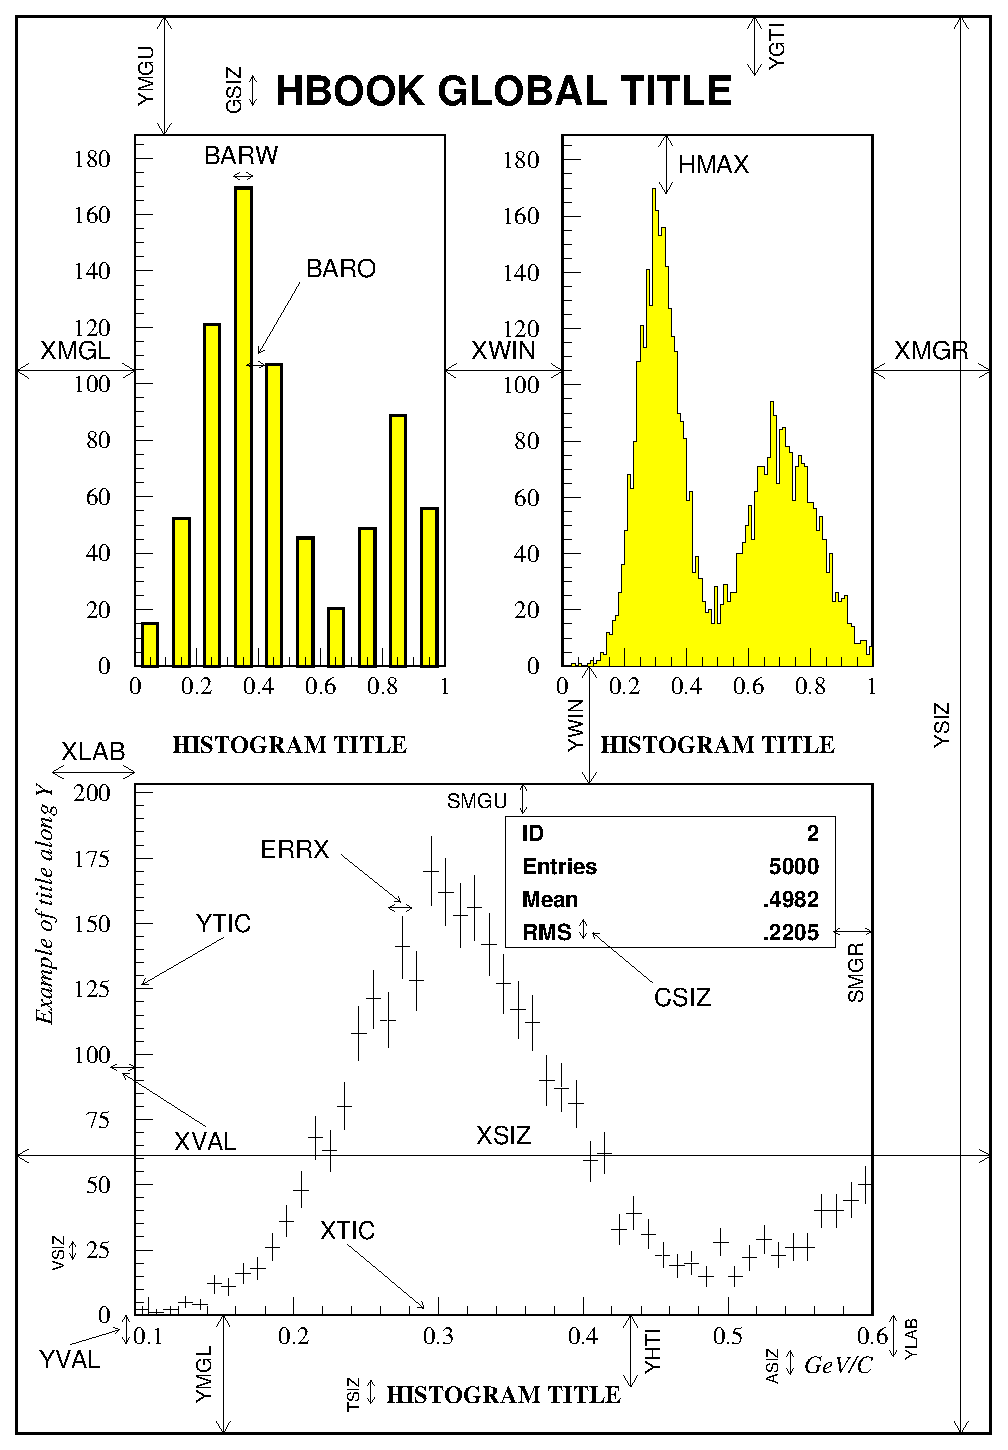
\includegraphics[width=.8\linewidth]{hplset.eps}
\caption{A graphical view of the {\tt SET} parameters}
\label{fig:HPLSET}
\end{figure}

\section{More on labels}
\index{alphanumeric!labels}
\index{label}

By default, labels used by \PAWcind{AXIS} and \PAWcind{PIE}
are numeric labels.
The command \PAWcind[LABELS]{GRAPHICS/PRIMITIVES/LABELS}
(or \PAWcind{LABELS} for short), allows the user to define
up to nine alphanumeric set of labels
(numbered from \texttt{1} to \texttt{9}).
These labels can then be used in subsequent commands
using \PAWcind{PIE} or \PAWcind{AXIS} primitives of HIGZ.

The \PAWcind{LABELS} command has three parameters:
\begin{DLtt}{123456}
\item[LABNUM] An integer between \texttt{1} and \texttt{9}.
              It identifies the labels set.
\item[NLABS]  The number of items to be placed on the labels 
              (up to \texttt{50}).
\item[CHLABS] \texttt{NLABS} character strings specifying the label items.
\end{DLtt}

The label sets thus defined can be used for axes on all plots produced
by PAW (HPLOT histograms, graphs, vectors drawing, etc.) via the
\PAWcind[SET]{SET NDVX (NDVY)} command.
\index{axis!divisions}
These commands have the following structure:

\subsection*{Example of \texttt{NXDV} specification}
\begin{alltt}
    SET \Ssind{NDVX} i            e.g. SET NDVX 512
{\rm or}
    SET \Ssind{NDVX} i.jk         e.g. SET NDVX 10.25
\end{alltt}

In the first case the number \texttt{i} contains
\texttt{100} times the 
number of secondary divisions plus the number of primary divisions.
(e.g. \texttt{512} means \texttt{12} primary and \texttt{5} secondary division. 
By adding \texttt{10000} times \texttt{N3} to \texttt{i} a third level of divisions
is available.
\index{divisions}

In the second case the number in front of the dot \texttt{(i)} indicates the total
number of divisions, the first digit following the dot \texttt{(j)} the label
identifier (\texttt{LABNUM}) (if this number is equal to \texttt{0} numeric labels
are drawn). The second digit after the \texttt{(k)} dot indicates the position 
where the \index{label!text justification} labels have to be drawn (i.e. the
{\em text justification} parameter, in this case \texttt{5}, indicating 
horizontally written text centered on the interval). Study figures 
\ref{fig:LABNDVX} and \ref{fig:LABNDVY} for details. These two figures show 
that the labels can be centered on the tick marks (\texttt{1} to \texttt{4}) or on 
the divisions (\texttt{5} to \texttt{8}). If the labels are centered on the tick 
marks, note that the number of items in the command \texttt{LABELS} must be equal
to the number of tick marks (which is equal to the number of divisions 
{\bf plus one}), otherwise the last alphanumeric label on the axis will be 
undefined. \index{tick marks}

By default, the number of primary divisions given by \PAWcind[SET]{SET NDVX n}, 
\PAWcind[SET]{SET NDVY n} or \PAWcind[SET]{SET NDVZ n} is optimized to have a 
reasonable labelling. The number of primary divisions is also optimized 
according the number of zones (command \PAWcind[ZONE]{ZONE}) i.e : 
along the X direction the number of primary divisions is divided by 
\texttt{the_number_of_X _zones} along the Y direction the number of primary 
divisions in divided by \texttt{(the_number_of_Y_zones)/2}.

If the number of divisions has to be exactly equal to the
number given by \PAWcind[SET]{SET NDVX n}, \PAWcind[SET]{SET NDVY n} or
\PAWcind[SET]{SET NDVZ n}, a negative value must be used i.e.:
\subsection*{Forcing an exact number of divisions}
\begin{alltt}
    SET \Ssind{NDVX} -i            e.g. SET NDVX -512
or
    SET \Ssind{NDVX} -i.jk         e.g. SET NDVX -10.25
\end{alltt}

For example to label each subsequent X-axis with the names of the
months of the year centered in the middle of each bin one can use:
\subsection*{Example of alphanumeric labels on an axis}
\begin{alltt}
PAW > \Ucom{LABEL 1 12 JAN FEB MAR APR MAY JUN JUL AUG SEP OCT NOV DEC}
PAW > \Ucom{SET NDVX -12.15}
\end{alltt}

\begin{figure}[p]
\centering\includegraphics[width=.74\linewidth]{ndvx.eps}
\caption{Example of labelling for horizontal axes}
\label{fig:LABNDVX}

\medskip

\centering\includegraphics[width=.74\linewidth]{ndvy.eps}
\caption{Example of labelling for vertical axes}
\label{fig:LABNDVY}
\end{figure}

\section{Colour, line width, and fill area in HPLOT}
\index{histogram!presentation}
\index{fill!area}
\index{colour}
\index{line!width}

The aspect of HPLOT pictures can be modified via the \texttt{xWID}, \texttt{xTYP}
and \texttt{xCOL} attributes, where \texttt{x} can be \texttt{H}, \texttt{B},
\texttt{P}, or \texttt{F}, defined as follows:
\begin{DLtt}{12}
\item[B] zone Box
\item[F] Function
\item[H] Histogram
\item[P] Page
\end{DLtt}

The values given to the parameters \Ssind{PTYP}, \Ssind{BTYP}, \Ssind{HTYP},
and \Ssind{FTYP} are the HIGZ fill area interior styles. Interior style
 provided by the basic graphics package (i.e. GKS) can be used (cf the
corresponding documentation) but in order to have the same result on all 
devices, numbers greater than \texttt{100} (HIGZ styles: \ref{fig:HATCH}) should
be used. Figure \ref{fig:BTYP} shows how to use the \texttt{xTYP} parameter. 

The parameters \Ssind{PCOL}, \Ssind{BCOL}, \Ssind{HCOL} and \Ssind{FCOL}
are equivalent to \Ssind{PTYP}, \Ssind{BTYP}, \Ssind{HTYP}, and \Ssind{FTYP}
respectively, but instead of changing the hatch style, they change the
colour of the same areas. It is possible to specify both the border and
the inside color for the Histogram, Box Page, and Function (\Ssind{HCOL}, 
\Ssind{BCOL}, \Ssind{PCOL}, \Ssind{FCOL}).
\subsection*{Example of \texttt{HCOL} specification}
\begin{alltt}
      Ex:
                  +---- 1 The Histogram is filled
                  |     0 Only the border is drawn 
                  |+--- Border color (here 2) if the histogram is filled
                  ||++- Inside color (here 3) if the histogram is filled
                  ||||  Border color if the histogram is not filled
                  ||||
                  VVVV
       SET  HCOL  1203  
\end{alltt}
The same mechanism is also available for \Ssind{FCOL}, \Ssind{BCOL} and 
\Ssind{PCOL}.

If \Ssind{PCOL}, \Ssind{BCOL}, \Ssind{HCOL} or \Ssind{FCOL} are between \texttt{1}
and \texttt{99}, then only the contour of the corresponding area is changed. 
If they are between \texttt{1001} and \texttt{1099}, then the surface is filled with
the colour determined by the corresponding fill area colour index (1 to 99).
If they are between \texttt{1199} and \texttt{1999}, then the surface is filled with
the colour determined by the corresponding fill area colour index (1 to 99)
and the border is drawn with the corresponding line color index (1 to 9).

If one of the \Ssind{*COL} is greater than 1000 the corresponding value of the
Fill Area Interior Style (for \Ssind{HTYP}, \Ssind{BTYP}, \Ssind{PTYP} or 
\Ssind{FTYP}) is automatically set to \texttt{1} (solid).

In addition, \Ssind{BCOL} has two digits after the dot. The first one specifies
the colour of the zone box shadowing and the second the colour
of the statistic box shadowing. 
\index{colour}

\section{Information about histograms}
\index{date!and hour on pictures}
\index{file name!on pictures}
\index{date}
\index{fit!parameters on pictures}
\index{statistic!parameters on pictures}

Four options are available to plot additional informations on HPLOT pictures:
\Oind{DATE}, \Oind{FILE}, \Oind{STAT} and \Oind{FIT}.

\begin{alltt}
PAW > \Ucom{OPTION DATE}        | Plot date and hour on current HPLOT picture
PAW > \Ucom{OPTION FILE}        | Plot file name of current histogram
PAW > \Ucom{OPTION STAT}        | Plot statistics of current histogram
PAW > \Ucom{OPTION FIT}         | Plot Fit parameters of current histogram
\end{alltt}

For each of these \PAWcind{OPTION} commands a corresponding 
\PAWcind{SET} parameter is available:

\begin{alltt}
PAW > \Ucom{SET DATE i}    | Default is 2
PAW > \Ucom{SET \Ssind{FILE} i}    | Default is 1
\end{alltt}
where \texttt{i} defines the position of the date or file name:

\begin{DLtt}{12345678}
\item[i = 1 :] Top left corner        of page/current histogram.
\item[i = 2 :] Top right corner
\item[i = 3 :] Bottom left corner
\item[i = 4 :] Bottom right corner
\end{DLtt}

For example the command:
\begin{alltt}
PAW > \Ucom{SET \Ssind{DATE} 3}
\end{alltt}
sets the position of the date to the bottom left corner of the HPLOT pictures.
\begin{alltt}
PAW > \Ucom{SET \Ssind{STAT} i}    | Default is 1111
\end{alltt}
where \texttt{i} corresponds to binary status bits \texttt{AOURMEI} as follows: 

\begin{DLtt}{1234}
\item[A=1] Draw the contents of all channels
\item[O=1] Draw number of overflows
\item[U=1] Draw number of underflows
\item[R=1] Draw R.M.S.
\item[M=1] Draw mean value
\item[E=1] Draw number of entries
\item[I=1] Draw histogram identifier
\end{DLtt}

For example the command:

\begin{alltt}
PAW > \Ucom{SET STAT 10}
\end{alltt}

sets the statistics informations to be only the number of entries.

\begin{alltt}
PAW > \Ucom{SET \Ssind{FIT} i}     | Default is 101
\end{alltt}
where \texttt{i} corresponds to binary status bits \texttt{CEP} as follows: 

\begin{DLtt}{123}
\item[C=1] Draw \(\chi^2\)
\item[E=1] Draw errors
\item[P=1] Draw fit parameters
\end{DLtt}

For example to draw only the result of the \(\chi^2\) fit one would use:
\begin{alltt}
PAW > \Ucom{SET FIT 100}
\end{alltt}

For all these \PAWcind{OPTION}s, the {\bf character size} is specified with the 
command \PAWcind[SET]{SET CSIZ} and the character font used with 
\PAWcind[SET]{SET CFON}.



\subsection*{Fill area style, marker and line type}

The Fill Area Interior Style, The Fill Area Style Index,
the Marker TYPe and the Line TYPe are set respectively using the
\PAWcind{IGSET} parameters
\Ssind{FAIS}, \Ssind{FASI}, \Ssind{MTYP} and \Ssind{LTYPE}.

\subsection*{Example}
\begin{alltt}
PAW > \Ucom{IGSET FAIS 3}      | Fill area are hatched
PAW > \Ucom{IGSET FASI 244}    |   with the style index
PAW > \Ucom{IGSET MTYP 25}     | Marker type is an empty square
PAW > \Ucom{IGSET LTYP 15}     | Line type is dotted
\end{alltt}
\index{hatch style}
\index{fill!area!style index}
\index{fill!area!interior style}
\index{marker!type}
\index{line!type}

HIGZ provides some portable fill area styles index coded
using three digits \texttt{ijk} as follows:

\begin{DLtt}{12}
\item[i:] Distance between each hatch in mm
\item[j:] Angle between \texttt{90} and \texttt{180} degrees
\item[k:] Angle between \texttt{0} and \texttt{90} degrees
\end{DLtt}

These numbers are coded according to table \ref{tab:HIGZSTY}
and examples are shown in figure \ref{fig:HATCH}.

\begin{table}
\[
\begin{array}{|crcrcr|}
\hline
\mbox{\tt i} &  \mathrm{Distance} &
\mbox{\tt j} &  \mathrm{Angle}    &
\mbox{\tt k} &  \mathrm{Angle}     \\
\hline
   &                               &
0  & 180^{\circ}                   &
0  &   0^{\circ}                   \\
1  & 0.75 \mathrm{mm}              &
1  & 170^{\circ}                   &
1  &  10^{\circ}                   \\
2  & 1.50 \mathrm{mm}              &
2  & 160^{\circ}                   &
2  &  20^{\circ}                   \\
3  & 2.25 \mathrm{mm}              &
3  & 150^{\circ}                   &
3  &  30^{\circ}                   \\
4  & 3.00 \mathrm{mm}              &
4  & 135^{\circ}                   &
4  &  45^{\circ}                   \\
5  & 3.75 \mathrm{mm}              &
5  & \multicolumn{1}{c}{\mbox{not drawn}} &
5  & \multicolumn{1}{c|}{\mbox{not drawn}} \\
6  & 4.50 \mathrm{mm}              &
6  & 120^{\circ}                   &
6  &  60^{\circ}                   \\
7  & 5.25 \mathrm{mm}              &
7  & 110^{\circ}                   &
7  &  70^{\circ}                   \\
8  & 6.00 \mathrm{mm}              &
8  & 100^{\circ}                   &
8  &  80^{\circ}                   \\
9  & 6.75 \mathrm{mm}              &
9  &  90^{\circ}                   &
9  &  90^{\circ}                   \\
\hline
\end{array}
\]
\caption{Codification for the HIGZ portable fill area interior styles}
\label{tab:HIGZSTY}
\end{table}

\subsection*{Example}
\begin{alltt}
PAW > \Ucom{IGSET FAIS 3}      | Fill area interior style is hatched
PAW > \Ucom{IGSET FASI 190}    | Hatch type is 190
\end{alltt}
These commands will yield hatching with two sets of lines
at $90^{\circ}$ and $0^{\circ}$ spaced 1 mm apart.

\begin{sidewaysfigure}
\begin{minipage}{.49\textheight}
\centering\includegraphics[height=14cm]{btyp.eps}
\caption{Usage of fill area types in HPLOT}
\label{fig:BTYP}
\end{minipage}\hfill
\begin{minipage}{.49\textheight}
\centering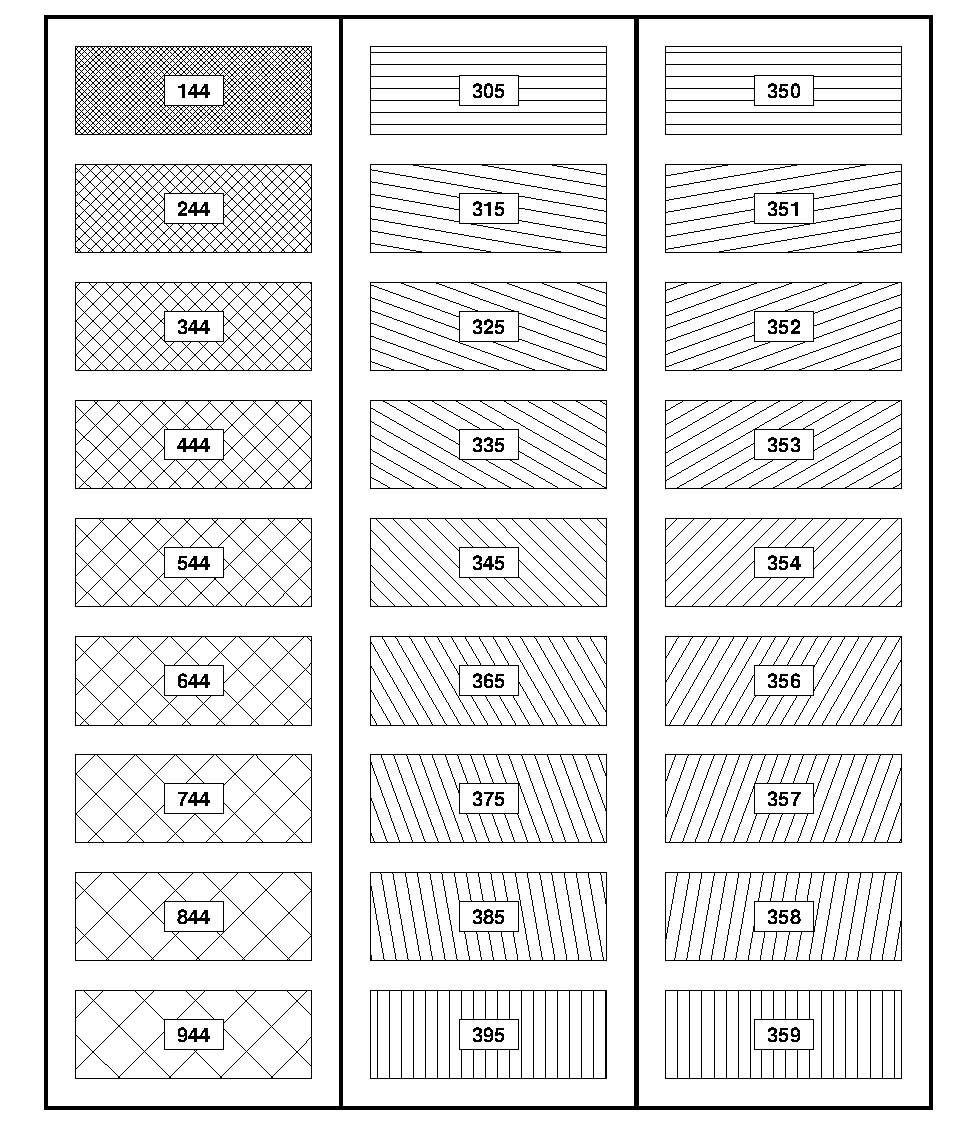
\includegraphics[height=14cm]{fasi.eps}
\caption{HIGZ portable hatch styles}
\label{fig:HATCH}
\index{hatch style}
\end{minipage}
\end{sidewaysfigure}

\begin{figure}[p]
\centering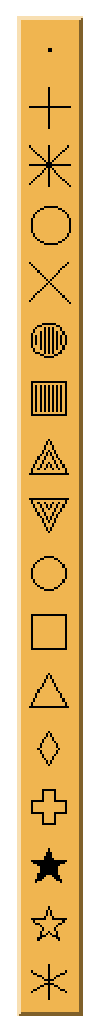
\includegraphics[width=12cm]{marker.eps}
\caption{HIGZ portable marker types}
\label{fig:MTYPE}
\index{marker!type}

\centering\includegraphics[width=10cm]{ltype.eps}
\caption{HIGZ portable line types}
\label{fig:LTYPE}
\index{line!type}

\centering\includegraphics[width=10cm]{greylev.eps}
\caption{PostScript grey level simulation of the basic colours}
\label{fig:GREYLEV}
\index{fonts}
\end{figure}

\section{Text drawing}
In PAW, text output can be produced in two ways:
\begin{enumerate}
\item {\em Automaticaly} with commands like \PAWcind{GRAPH} or 
      \PAWcind{HISTO/PLOT} in which a lot of text is drawn: the axis labels, the
      histogram title, the global title, the statistics etc. . The attributes
      (font, colour or size) and the placement of these texts are controled 
      with the command \PAWcind{SET}. In the rest of the chapter, the text
      produce {\em automaticaly} will be called {\em HPLOT text}
\item {\em Directly} with the commands \PAWcind{ITX} and \PAWcind{TEXT}. The 
      attributes of \PAWcind{ITX} are controlled with the command 
      \PAWcind{IGSET} whereas the attributes of \PAWcind{TEXT} are given
      with the command parameters.
\end{enumerate}

\subsection*{Text placement}
The text placement specify where the text must be drawn. For the
{\em HPLOT text}, the text position  is always in centimeters whereas for
\PAWcind{ITX} or \PAWcind{TEXT} the current coordinate system is used. 
\subsubsection{HPLOT text}
The possible text placements for {\em HPLOT text} are described in the
following example:
\begin{alltt}
PAW > \Ucom{SET XVAL 0.40} | distance between the Y axis and the axis values
PAW > \Ucom{SET YVAL 0.20} | distance between the X axis and the axis values
PAW > \Ucom{SET YLAB 0.80} | distance X axis to labels
PAW > \Ucom{SET XLAB 1.40} | distance Y axis to labels
PAW > \Ucom{SET YGTI 1.50} | Y position of global title
PAW > \Ucom{SET YHTI 1.20} | Y position  of histogram title
PAW > \Ucom{SET YNPG 0.60} | Y position for the page number
PAW > \Ucom{HISTO/PLOT 10} | the histogram 10 is drawn with previous settings
\end{alltt}
See figure \ref{fig:HPLSET} for more details.
\subsubsection{ITX}
In the command \PAWcind{ITX} the text position is defined with two mandatory
parameters (\texttt{X} and \texttt{Y}): 
\begin{alltt}
PAW > \Ucom{SELNT 1}         | cm coordinates
PAW > \Ucom{ITX 5 5 'Hello'} | 'Hello' is drawn at the position (5,5)
\end{alltt}
\subsubsection{TEXT}
In the command \PAWcind{TEXT} the text position is defined with two mandatory
parameters (\texttt{X} and \texttt{Y}): 
\begin{alltt}
PAW > \Ucom{SELNT 1}            | cm coordinates
PAW > \Ucom{TEXT 5 5 'Hello' 1} | 'Hello' is drawn at the position (5,5)
\end{alltt}

\subsection*{Text size}
For all the texts drawn with PAW commands, the text size is always specified
in centimeters.
\subsubsection{HPLOT text}
The possible text sizes for {\em HPLOT text} are described in the
following example:
\begin{alltt}
PAW > \Ucom{SET ASIZ 0.28} | axis label size
PAW > \Ucom{SET CSIZ 0.28} | comment size
PAW > \Ucom{SET GSIZ 0.28} | global title size
PAW > \Ucom{SET KSIZ 0.28} | Hershey character size
PAW > \Ucom{SET 2SIZ 0.28} | scatter plot and table character. size
PAW > \Ucom{SET TSIZ 0.28} | histogram title size
PAW > \Ucom{SET VSIZ 0.28} | axis values size
PAW > \Ucom{HISTO/PLOT 10} | the histogram 10 is drawn with previous settings
\end{alltt}
See figure \ref{fig:HPLSET} for more details.
\subsubsection{ITX}
The text character heigh attribute for use by future invocations of 
\PAWcind{ITX} is set using the \Ssind{CHHE} parameter as follows:
\begin{alltt}
PAW > \Ucom{IGSET CHHE 1}    | set the character heigh to 1 cm.
PAW > \Ucom{ITX 5 5 'Hello'} | the size of 'Hello' is 1 cm.
\end{alltt}
\subsubsection{TEXT}
In the command \PAWcind{TEXT} the text size is a mandatory parameter
(\texttt{SIZE}).
\begin{alltt}
PAW > \Ucom{TEXT 5 5 'Hello' 1} | the size of 'Hello' is 1 cm.
\end{alltt}

\subsection*{Text orientation}
The text orientation is an angle (in degrees) between the \texttt{X} axis
and the text axis. By default this angle is equal to 0.
\subsubsection{HPLOT text}
Text orientation cannot be changed with some \PAWcind{SET} parameters for the
{\em HPLOT text}. It is always automaticaly computed. For example in
the command \PAWcind{ATITLE}, which draws the axis titles, the title
on the \texttt{Y} axis is automaticaly drawn with an angle of 90 degrees.
\subsubsection{ITX}
The text orientation attribute for use by future invocations of 
\PAWcind{ITX} is set using the \Ssind{TANG} parameter as follows:
\begin{alltt}
PAW > \Ucom{IGSET TANG 90}   | set the text angle to 90 degrees.
PAW > \Ucom{ITX 5 5 'Hello'} | 'Hello' is drawn with an angle of 90 degrees.
\end{alltt}
\subsubsection{TEXT}
In the command \PAWcind{TEXT} the text orientation is an optional parameter
(\texttt{ANGLE}).
\begin{alltt}
PAW > \Ucom{TEXT 5 5 'Hello' ! 90} | 'Hello' is drawn with an angle of 90 degrees
\end{alltt}

\subsection*{Text alignment}
\index{text!alignment!horizontal}
\index{text!alignment!vertical}
The text alignment controls the placement of the character string  with 
respect to the specified text position.
\subsubsection{HPLOT text}
Text alignment cannot be changed for the
{\em HPLOT text}. It is automaticaly computed.
\subsubsection{ITX}
The text alignment attributes for use by future invocations of \PAWcind{ITX}
are set using the \Ssind{TXAL} parameter as follows:
\begin{alltt}
PAW > \Ucom{IGSET TXAL (10*(horizontal alignment) + (vertical alignment))}
\end{alltt}
The horizontal and 
vertical alignments parameters must be in the range \texttt{0-3}. The horizontal 
alignment specifies which end of the string (or its geometric center) is 
aligned with the specified point given in \PAWcind{ITX}.
The vertical alignment controls whether the top of tall characters
(or the bottom of capital letters) line up with the specified point 
(see figure \ref{fig:ALIGN}).
\begin{itemize}
\item[ITXALH] horizontal alignment
\begin{itemize}
\item[0] normal (usually same as 1)
\item[1] left end of string at specified point
\item[2] center of string at specified point
\item[3] right end of string at specified point
\end{itemize}
\item[ITXALH] vertical alignment
\begin{itemize}
\item[0] normal
\item[1] top of tallest chars plus any built in spacing
\item[2] top of tallest chars
\item[3] halfway between 2 and 4 
\end{itemize}
\end{itemize}
\begin{figure}
\centering\includegraphics[width=12cm]{align.eps}
\caption{Text alignment}
\label{fig:ALIGN}
\index{text alignment}
\end{figure}
\begin{alltt}
PAW > \Ucom{IGSET TXAL 23}   | The horizontal and vertical alignments are centered
PAW > \Ucom{ITX 5 5 'Hello'} | 'Hello' is drawn center adjusted
\end{alltt}
\subsubsection{TEXT}
In the command \PAWcind{TEXT} the text alignment is an optional parameter
(\texttt{CHOPT}). Only the horizontal alignment can be changed among three 
possible values: Left, Center or Right.
\begin{alltt}
PAW > \Ucom{TEXT 5 5 'Hello' 1 ! L} | 'Hello' is drawn left adjusted (default)
PAW > \Ucom{TEXT 5 5 'Hello' 1 ! C} | 'Hello' is drawn center adjusted
PAW > \Ucom{TEXT 5 5 'Hello' 1 ! R} | 'Hello' is drawn right adjusted
\end{alltt}

\subsection*{Text colour}
The text colour is define via a colour index in the colour table.
\subsubsection{HPLOT text}
\begin{alltt}
PAW > \Ucom{SET XCOL 2}    | X axis color
PAW > \Ucom{SET YCOL 3}    | Y axis color
PAW > \Ucom{HISTO/PLOT 10} | the histogram 10 is drawn with previous settings
\end{alltt}
\subsubsection{ITX}
The text colour attribute for use by future invocations of 
\PAWcind{ITX} is set using the \Ssind{TXCI} parameter as follows:
\begin{alltt}
PAW > \Ucom{IGSET TXCI 3}    | set the text colour to green.
PAW > \Ucom{ITX 5 5 'Hello'} | 'Hello' is drawn in green.
\end{alltt}
\subsubsection{TEXT}
The text colour attribute for use by future invocations of 
\PAWcind{TEXT} is set using the \Ssind{TXCI} parameter as follows:
\begin{alltt}
PAW > \Ucom{IGSET TXCI 2}       | set the text colour to red.
PAW > \Ucom{TEXT 5 5 'Hello' !} | 'Hello' is drawn in red.
\end{alltt}

\subsection*{Text font and precision}
\index{font!text}
\index{text!font}
\index{text!precision}
\index{precision!text}
Text font selects the desired character font e.g. a roman font, a sans-serif 
font, etc. Text precision specifies how closely the graphics package 
implementation must follow the current size and orientation attributes. 
String (\texttt{0}) precision is most liberal (hardware), stroke (\texttt{2}) 
precision is most strict. Character precision is in the middle (\texttt{1}). 
The value of text font is dependent upon the basic graphics package used. 
However, font number \texttt{0}, with precision \texttt{2} is always available,
independently from the basic graphics package used.% (see figure \ref{fig:SOFT}).
Hardware characters are available with all the basic graphics packages. With
X11, a large variety of font is available. They are the same as the PostScript
fonts (see figure \ref{PS-FONT}).

\subsubsection{HPLOT text}
\begin{alltt}
PAW > \Ucom{SET CFON -60}  | comment font is Helvetica Bold
PAW > \Ucom{SET GFON -20}  | global title font is Times Bold
PAW > \Ucom{SET LFON -60}  | axis labels font is Helvetica Bold
PAW > \Ucom{SET TFON -20}  | general comments is Times Bold
PAW > \Ucom{SET VFON -60}  | axis values font is Helvetica Bold
PAW > \Ucom{HISTO/PLOT 10} | the histogram 10 is drawn with previous settings
\end{alltt}
Note that \texttt{SET *FON ffp} set all the {\em HPLOT text} font to the
same value \texttt{ffp}.

\subsubsection{ITX}
Text font and precision attributes for use by later
invocations of \PAWcind{ITX} are set with \Ssind{TXFP} as follows:
\begin{alltt}
PAW > \Ucom{IGSET TXFP (10*(Text font) + (text precision))}
\end{alltt}

\subsubsection{TEXT}
This command draws a software character text, independently from the basic
graphics package used by HIGZ. It can produce over 300 different graphic signs.
The way in which software characters are defined is via a string of valid
characters, intermixed by other characters, acting as ``escape'' characters
\index{character!escape} (e.g. a change of alphabet, upper or lower case). The
string is interpreted by \PAWcind{TEXT} and the resulting characters are 
defined according to the figure~\ref{SOFTTEXT}, which shows the list of 
available software characters. This command allows the user to mix different
types of characters (roman, greek, special, upper and lower case, sub and 
superscript). There are a total of 10 control characters.

\index{lower case letters}
\index{upper case letters}
\index{Greek letters}
\index{superscript}
\index{subscript}
\index{backspace}
\index{termination character}
\index{special symbols}
\label{ESCCHAR}
\begin{tabular}{||c|p{7cm}||c|p{7cm}||}
\hline
\multicolumn{4}{|c|}{\bf List of escape characters and their meaning}      \\
\hline
 $<$  & go to lower case                 & $>$  & go to upper case (default) \\
\hline
 \lsb & go to greek (Roman = default)    & \rsb & end of greek               \\
\hline
 "    & go to special symbols            & \#   & end of special symbols     \\
\hline
$\uparrow$  & go to superscript         & ?    & go to subscript            \\
\hline
 !    & go to normal level of script     & \&   & backspace one character    \\
\hline
 \$   & termination character (optional) &      &                            \\
\hline
\end{tabular}

Note that characters can be also entered directly in lower case or upper case
instead of using the control characters {\tt <} and {\tt >}.

The boldface characters may be simulated by setting the
attributes '\Sind{PASS}' and '\Sind{CSHI}' with \PAWcind{IGSET}.
The meaning of these attributes is the
following: Every stroke used to display the character is repeated
\Sind{PASS} times, at a distance (in percentage of the character height)
given by \Sind{CSHI}.

\begin{figure}
\centering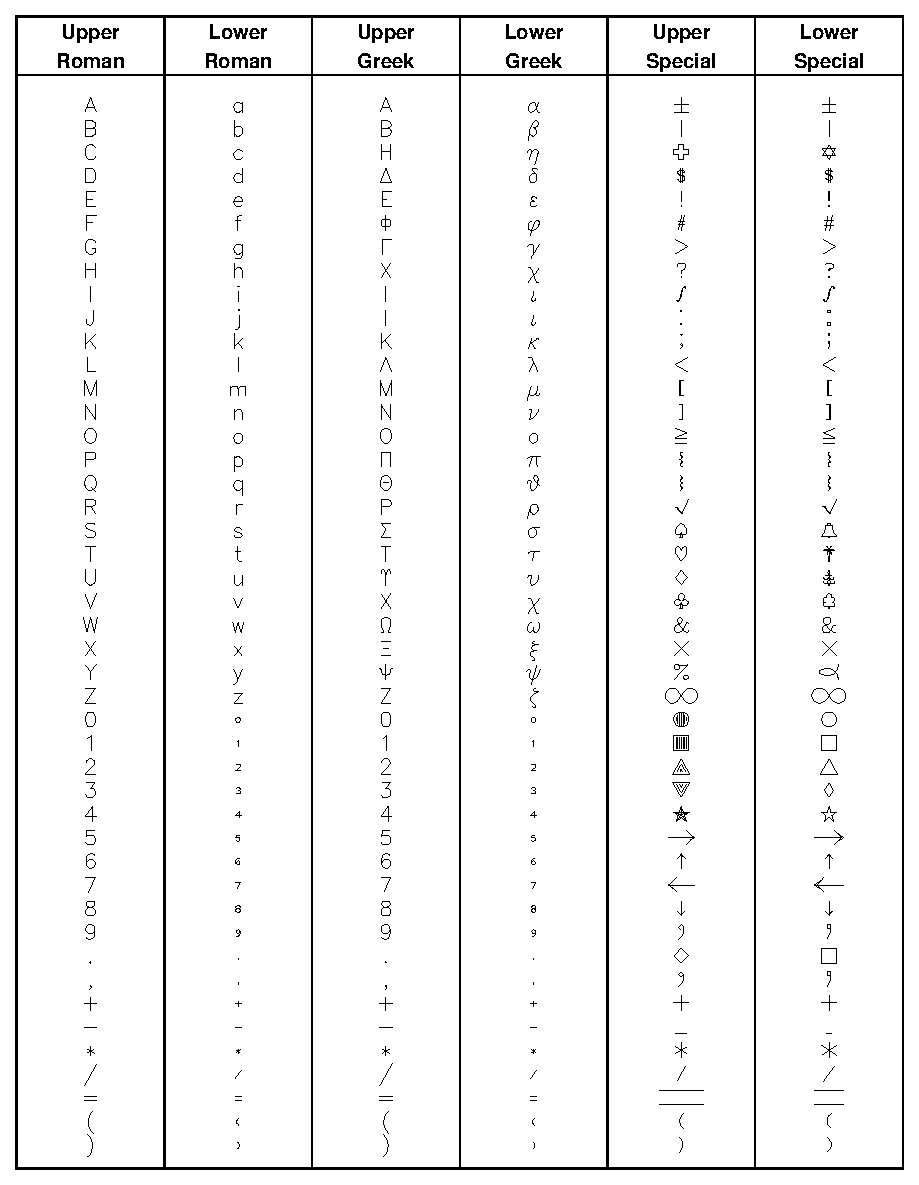
\includegraphics[width=.8\linewidth]{softtext.eps}
\caption{Characters available in \texttt{IGTEXT}}
\label{SOFTTEXT}
\end{figure}

\subsubsection{PostScript text fonts}
\index{font!PostScript}
\index{PostScript!fonts}
\index{PostScript!fonts!Times-Italic}
\index{PostScript!fonts!Times-Bold}
\index{PostScript!fonts!Times-BoldItalic}
\index{PostScript!fonts!Helvetica}
\index{PostScript!fonts!Helvetica-Oblique}
\index{PostScript!fonts!Helvetica-Bold}
\index{PostScript!fonts!Helvetica-BoldOblique}
\index{PostScript!fonts!Courier}
\index{PostScript!fonts!Courier-Oblique}
\index{PostScript!fonts!Courier-Bold}
\index{PostScript!fonts!Courier-BoldOblique}
\index{PostScript!fonts!Symbol}
\index{PostScript!fonts!Times-Roman}
\index{PostScript!fonts!ZapfDingbats}

PostScript files the text can be generated with PostScript fonts. The figure 
\ref{PS-FONT} shows all the PostScript fonts available on most PostScript 
printers. Note that the fonts {\tt -15} to {\tt -24} are the same than 
{\tt -1} to {\tt -14}, but they are drawn in hollow mode.

The correspondence between ASCII and {\sf ZapfDingbats} font
is given on figures \ref{PSTEXT1} and \ref{PSTEXT2}.
\PAWcind{TEXT} control characters are taken into account. In addition
the character $\sim$ switches to the {\sf ZapfDingbats} character set.
\index{lower case letters}
\index{upper case letters}
\index{Greek letters}
\index{superscript}
\index{subscript}
\index{backspace}
\index{termination character}
\index{special symbols}
\begin{center}
\begin{tabular}{||c|l||c|l||}
\hline
\multicolumn{4}{|c|}{\bf List of escape characters and their meaning}      \\
\hline
 $<$  & go to lower case (optional)      & $>$  & go to upper case (optional)\\
\hline
 \lsb & go to greek (Roman = default)    & \rsb & end of greek               \\
\hline
 "    & go to special symbols            & \#   & end of special symbols     \\
\hline
$\sim$ & go to ZapfDingbats               & \#   & end of ZapfDingbats        \\
\hline
$\uparrow$  & go to superscript          & ?    & go to subscript            \\
\hline
 !    & go to normal level of script     & \&   & backspace one character    \\
\hline
 \$   & termination character (optional) &      &                            \\
\hline
\end{tabular}
\end{center}
\par
The PostScript fonts can be used with precision {\tt 0} or precision {\tt 1}.
On the screen, a PostScript font used with precision {\tt 1} appears
like the \PAWcind{TEXT} characters, with precision 0 its appears as
hardware character (X11 fonts). In both cases the  PostScript file is the same.

Note that characters can also be entered directly in lower or upper case
instead of using the escape characters {\tt <} and {\tt >}.
Examples of PostScript text and math are shown in Figures~\ref{PSEX1}
and \ref{PSEX2}.

\begin{figure}
\begin{salltt}
PAW > IGSET LWID 6
PAW > BOX 0 16 0 5 
PAW > IGSET CHHE 0.5
PAW > IGSET TXAL 3
PAW > IGSET TXFP -130
PAW > ITX 3 4 'K\bs{}355nstler in den gr\bs{}345\bs{}373ten st\bs{}311dten
PAW > ITX 3 3 '\bs{}253\bs{}265 l''\bs{}372uvre on conna\bs{}333t l''artisan\bs{}273
PAW > ITX 3 2 '\bs{}(proverbe fran\bs{}321ais\bs{}
PAW > ITX 3 1 '\bs{}252\bs{}241Ma\bs{}337ana\bs{}41 \bs{}322ag&\bs{}306!das&\bs{}313!\bs{}272, dit l''\bs{}323l\bs{}325ve.
\end{salltt}
\begin{center}
\includegraphics[width=.7\linewidth]{psex1.eps}
\end{center}
\caption[PostScript text]
        {Example of PostScript text (result of input above)}
\label{PSEX1}

\bigskip

\begin{salltt}
PAW > IGSET LWID 6
PAW > BOX 0 16 0 5
PAW > IGSET CHHE 0.5
PAW > IGSET TXAL 23
PAW > IGSET TXFP -130
PAW > ITX 8 4 'e^+!e^-! "5# Z^o! "5# ll&^-!, qq&^\bs{}261!'
PAW > ITX 8 3 '| a&^[\bs{}256]! \bs{}267 b&^[\bs{}256]! | = [\bs{}345] a^i?&jk!+b^kj?&i'
PAW > ITX 8 2 'i ("d#?[m!y]&^\bs{}261![g^m]! + m [y]&^\bs{}261! ) = 0" r# (~r# + m^2!) [y] = 0'
PAW > ITX 8 1 'L?em! = e J^[m]?&em! A?[m]! , J^[m]?&em!=l&^\bs{}261![ g?m]!l , M^j?&i! = [\bs{}345&?a]! A?[a! t^a]j?&i! '
\end{salltt}
\begin{center}
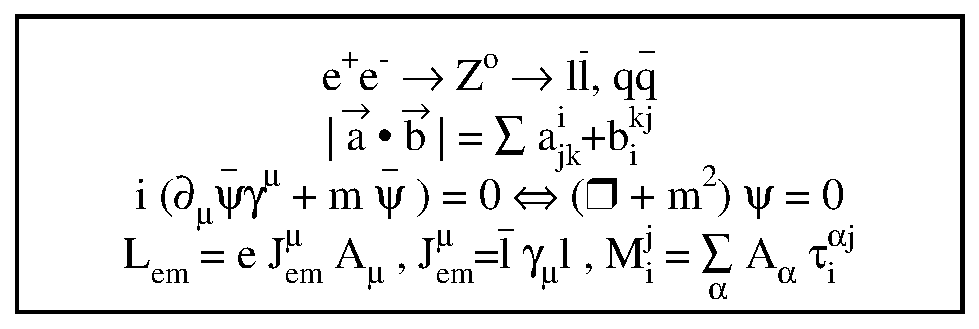
\includegraphics[width=.7\linewidth]{psex2.eps}
\end{center}
\caption[PostScript text and maths]%
        {Example of PostScript text and maths (result of input above)}
\label{PSEX2}
\end{figure}

\begin{figure}
\centering\includegraphics[width=\linewidth]{psfont.eps}
\caption{PostScript text fonts.}
\label{PS-FONT}
\end{figure}

\begin{figure}
\centering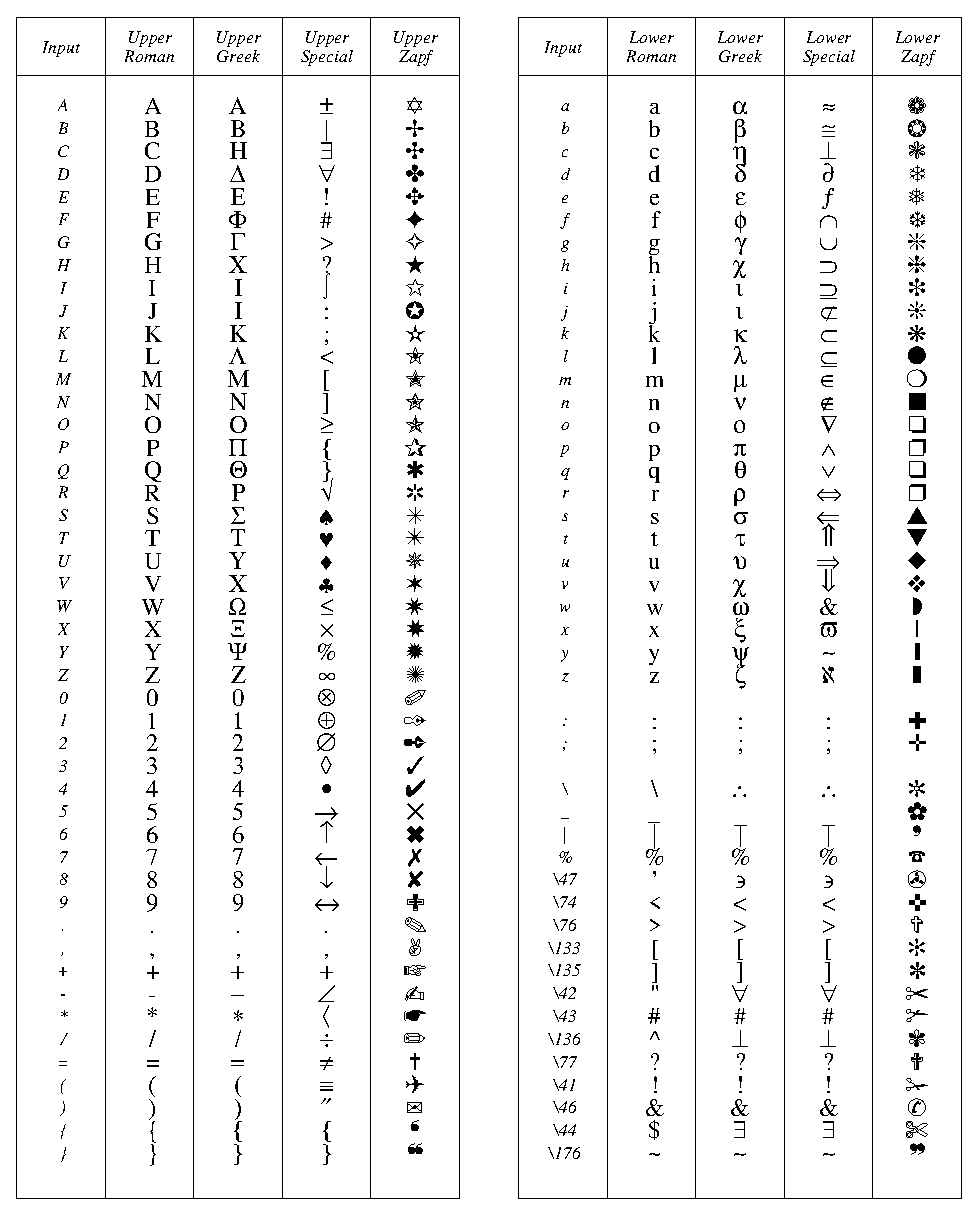
\includegraphics[width=\linewidth]{pstext1.eps}
\caption{PostScript characters (1).}
\label{PSTEXT1}
\end{figure}

\begin{figure}
\centering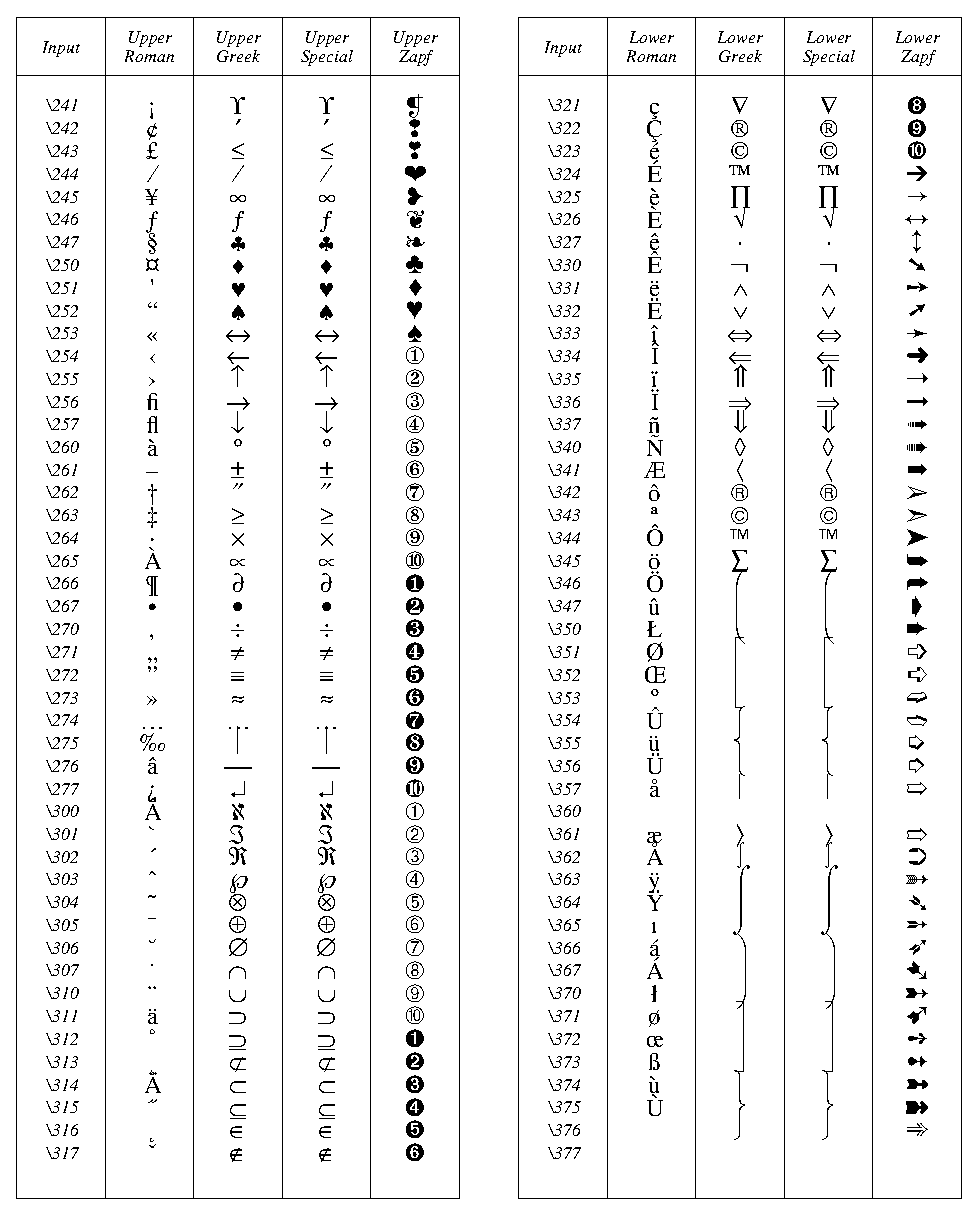
\includegraphics[width=\linewidth]{pstext2.eps}
\caption{PostScript characters (2).}
\label{PSTEXT2}
\end{figure}

\clearpage
\section{The HIGZ graphics editor}
\index{graphics!editor}
\index{editor}
\index{HIGZ!graphics editor}

The HIGZ pictures in memory can be modified interactively with the HIGZ
graphics editor. 
The command \PAWcind[MODIFY]{PICT/MODIFY} invokes the HIGZ editor
(see figure \ref{fig:GEDIFIG} for more details):
\begin{alltt}
PAW > \Ucom{PICT/MODIFY PNAME}
\end{alltt}
\texttt{PNAME} can be the complete name, the picture number in memory
or \texttt{' '}.

\begin{figure}
\includegraphics[width=\linewidth]{gedifig.eps}
\caption{The HIGZ graphics editor}
\label{fig:GEDIFIG}
\end{figure}

\endinput
%%%%%%%%%%%%%%%%%%%%%%%%%%%%%%%%%%%%%%%%%%%%%%%%%%%%%%%%%%%%%%%%%%%%%%%%%%%%%%%%
%                                                                              %
%   PAW   - Reference Manual -- LaTeX Source                                   %
%                                                                              %
%   Chapter 9: Distributed PAW                                                 %
%                                                                              %
%   Editor: Michel Goossens / IT-ASD                                           %
%   Last Mod.: 31 July 1998 Olivier Couet                                      %
%                                                                              %
%%%%%%%%%%%%%%%%%%%%%%%%%%%%%%%%%%%%%%%%%%%%%%%%%%%%%%%%%%%%%%%%%%%%%%%%%%%%%%%%

\chapter{Distributed PAW}
\label{sec:H1DIST}
 
\section{Access to remote files from a PAW session}
 
\index{remote!file}
\index{remote!shell}
\index{remote!login}
\index{RSHELL}
\index{RLOGIN}
When running PAW, it is often necessary to access files
(e.g. HBOOK files) which reside on a different computer. 
The ZFTP program described
above can be used if a very frequent access to the file is required. A
more convenient mechanism is the possibility to access the 
files directly. On many systems, one may now use \texttt{NFS}~\cite{bib-NFS}
for this purpose. Under some circumstances, for example if the HBOOK
file is not in exchange mode and it is to be accessed from a computer
running a different operating system, an alternate approach is required.
To fill this gap the PAW server is provided. This works using
a conventional Client/Server model. The client
(PAW) typically runs on a workstation. When the PAW command RLOGIN is invoked,
a PAW server is automatically started on the remote machine, normally
a mainframe or data server. 
 
Once the \texttt{RLOGIN REMOTE} command has been executed, the PAW Current Directory
is set to \texttt{//REMOTE}. The PAW client can now instruct the PAW server to
attach a file using the \texttt{RSHELL} command (e.g. \texttt{rshell file pawtest.dat}). If an
histogram with HBOOK ID=10 is on the remote file, than the PAW command
\texttt{Histo/Plot 10}
will plot this histogram on the local workstation. The histogram resides
on \texttt{//PAWC} like other histograms coming from local files.
 
The \texttt{RSHELL} command may be used to communicate with the PAW server.
The expression typed following \texttt{RSHELL} is passed to the server. The current
implementation of the PAW server recognizes the commands:
\begin{DLtt}{123456789012345678890}
\item[rshell file filename]Server connects filename
\item[rshell cdir //lun11] Server changes current directory
\item[rshell ld]           Server lists current directory
\item[rshell ld //]        Server lists all connected files
\item[rshell message]      Server pass message to operating system
\end{DLtt}
 
\subsection*{Access to remote files from a workstation}
\begin{alltt}
PAW > \Ucom{rlogin CERNVM}                         | connect to CERNVM
PAW > \Ucom{rshell file HRZTEST.DAT}               | PAW server connects HRZTEST DAT A to //LUN11
PAW > \Ucom{histo/plot 10}                         | plot histogram 10 from CERNVM
PAW > \Ucom{histo/fit 20 G}                        | fit histo 20 with a gaussian and plot it
PAW > \Ucom{rlogin VXCRNA}                         | connect to VXCRNA
PAW > \Ucom{rshell file DISK$DL:[PAW]HEXAM.DAT;3}  | PAW server on VXCRNA connects file to //LUN11
PAW > \Ucom{histo/plot 110}                        | plot histogram 110 from VXCRNA
PAW > \Ucom{rshell file HRZTEST.DAT}               | PAW server on VXCRNA connects file to //LUN12
PAW > \Ucom{histo/plot 110 s}                      | plot histogram 110 from HRZTEST.DAT
                                            | on VXCRNA on the existing picture
PAW > \Ucom{rshell ld //}                          | list all files connected on VXCRNA
PAW > \Ucom{cdir //CERNVM}                         | Change current PAW directory to CERNVM
PAW > \Ucom{histo/plot 110}                        | plot histogram 110 from CERNVM
PAW > \Ucom{histo/plot //VXCRNA/110}               | plot histogram 110 from VXCRNA
PAW > \Ucom{cdir //PAWC}                           | current directory to local memory
PAW > \Ucom{histo/list}                            | list all histograms in //PAWC
PAW > \Ucom{Histo/delete 0}                        | delete all histograms in memory
PAW > \Ucom{hrin //VXCRNA/0}                       | read all histograms from VXCRNA
                                            | file HRZTEST.DAT to //PAWC
PAW > \Ucom{cdir //CERNVM}                         | change directory to CERNVM
PAW > \Ucom{rshell file NEW.DAT.D 1024 N}          | creates a new file on the D disk
PAW > \Ucom{hrout 0}                               | write all histograms from //PAWC
                                            | to CERNVM file NEW DAT D
\end{alltt}
 
\newpage

\section{Using PAW as a presenter on VMS systems (global section)}
 
 
\index{global!section}
\index{VMS}
\index{presenter}
In addition to the facilities described in the previous section,
the standard version of PAW may be used as an online presenter
on VMS systems using the mechanism of global sections.
It is possible for two processes to reference the same histograms
using {\bf global sections}.
\index{global!section}
\index{VAX/VMS}
For example, the first process may be a {\bf histogram producer}
(e.g. a monitoring task) and the second process  {\bf PAW}.
As the
histograms are being gradually filled by the first task, PAW can
view them, and even reset them.
To use the global sections, it is also necessary to "page align" the common
which is in the global section. This is achieved in the "link step" when making
the process (see example).
The relevant statements are \texttt{SYS\$INPUT/OPTIONS}
to tell the linker that some options follow the link statement,
and \texttt{PSECT=PAWC,PAGE} which is the option to
page align the \texttt{/PAWC/} common.
 
\begin{minipage}{.48\textwidth}
\begin{alltt}
      PROGRAM PRODUCE
      PARAMETER MAXPAGES=100
      COMMON/PAWC/IPAWC(128*MAXPAGES)
      CHARACTER*8 GNAME
      INTEGER*4 HCREATEG
*
      GNAME='GTEST'
      WAIT_TIME=1.
      NUMEVT=1000
*...............           Create Global section
      NPAGES=HCREATEG(GNAME,IPAWC,128*MAXPAGES)
      IF(NPAGES.GT.0) THEN
         PRINT 1000,GNAME
 1000    FORMAT(' Global Section: ',A,' created')
      ELSE
         IERROR=-NPAGES
         PRINT 2000,IERROR
 2000    FORMAT(' Global Section Error', I6)
         GO TO 99
      ENDIF
      CALL HLIMIT(128*NPAGES)
*...............           Book histos.
      CALL HBOOK1(10,'Test1$',50,-4.,4.,0.)
      CALL HBOOK1(20,'Test2$',50,-4.,4.,0.)
*...............           Fill histos.
      DO 20 I=1,NUMEVT
         DO 10 J=1,100
            CALL RANNOR(A,B)
            CALL HFILL(10,A,0.,1.)
            CALL HFILL(20,B,0.,1.)
 10      CONTINUE
        CALL LIB$WAIT(WAIT_TIME)
 20   CONTINUE
*
 99   STOP
      END
 
$ fort produce
$ link produce,SYS$INPUT/OPTIONS,-
cern$library:packlib/lib,kernlib/lib
PSECT=PAWC,PAGE
\end{alltt}
\end{minipage}\hfill
\begin{minipage}{.50\textwidth}
\begin{alltt}
    PAW > \Ucom{edit produce}
       macro produce ntimes=100
         nt=[ntimes]
         zone 1 2
         histo/plot 10 K
         histo/plot 20 K
       loop:
           histo/plot 10 U
           histo/plot 20 U
           wait ' ' 1
           nt=[nt] -1
           if nt>0 goto loop
       return
    PAW > \Ucom{global GTEST}
    PAW > \Ucom{exec produce ntimes=20}
\end{alltt}
\includegraphics[width=\textwidth]{pawglob.eps}
\end{minipage}
\newpage

\section{Using PAW as a presenter on OS9 systems}
 
\index{presenter}
\index{OS9}
\index{TCP/IP}
\index{remote!login}
\index{remote!shell}
\index{RLOGIN}
\index{RSHELL}
\index{client}
\index{server}
\index{PAW!server}
The technique described in previous sections may also be used
to access HBOOK histograms being filled by a monitoring task
on OS9 systems from a standard PAW session running
on a machine with the TCP/IP software.
 
\begin{minipage}{.48\textwidth}
\begin{alltt}
      INDIRECT PAWC
      PROGRAM PRODUCE
*
*        Monitoring task MT1 in processor OP2.
*
      PARAMETER NWPAW=10000
      COMMON/PAWC/IPAWC(NWPAW)
*
      CALL HLIMIT(NWPAW)
*
*       Book histos.
*
      CALL HBOOK1(10,'TEST1$',50,-3.,3.,0.)
      CALL HBOOK1(20,'TEST2$',50,-3.,3.,0.)
*
*       Fill histos.
*
      NUMEVT=10000
      DO 20 I=1,NUMEVT
         DO 10 J=1,100
            CALL RANNOR(A,B)
            CALL HFILL(10,A,0.,1.)
            CALL HFILL(20,B,0.,1.)
 10      CONTINUE
 20   CONTINUE
*
 99   STOP
      END
\end{alltt}
\end{minipage}\hfill
\begin{minipage}{.50\textwidth}
\epsfig{file=pawos9.eps,width=\the\textwidth}
\end{minipage}
\bigskip
 
\subsection*{Example of how to access OS9 modules from PAW}
\begin{alltt}
PAW > \Ucom{rlogin O-OPAL01}                            | connect to an OS9 machine
PAW > \Ucom{rshell module OP2/MT1}                      | PAW server connects to OP2/MT1
                                                 | (Processor OP2, Monitoring Task MT1)
PAW > \Ucom{histo/plot 10}                              | plot histogram 10
PAW > \Ucom{hrin 0}                                     | read all histograms into //PAWC
PAW > \Ucom{Histo/File 1 local.dat 1024 N}              | create a new file local.dat
                                                 | on the client machine
PAW > \Ucom{hrout 0}                                    | save all histograms from //PAWC
                                                 | to the local file
PAW > \Ucom{rshell module OP3/MT2}                      | PAW server connects to another
                                                 | OS9 monitoring task
PAW > \Ucom{Output 56 os9.listing}                      | Change output file on client
PAW > \Ucom{rshell ldir}                                | list all histograms in MT2
                                                 | on file os9.listing
PAW > \Ucom{Output -56 }                                | Change output file to default (unit 6)
                                                 | file os9.listing is closed
\end{alltt}
\endinput

\include{pawch11}
%%%%% **************** Start of part 3 **************************-- >
%%%\part{PAW - Reference section}
%%%%%%%%%%%%%%%%%%%%%%%%%%%%%%%%%%%%%%%%%%%%%%%%%%%%%%%%%%%%%%%%%%%%
%    Explanation about notation for Reference Guide                %
%%%%%%%%%%%%%%%%%%%%%%%%%%%%%%%%%%%%%%%%%%%%%%%%%%%%%%%%%%%%%%%%%%%%
%%%\framebox[\textwidth][t]{\hfill\begin{minipage}{0.93\textwidth}%
%%%\vspace*{3mm}
%%%\begin{center}
%%%Notation used in the reference section
%%%\end{center}
%%%\parskip\baselineskip
 
%%%{\bf Optional} parameters are enclosed in square brackets, e.g.
%%%\Lit{[optpar]}
 
%%%The {\bf type} of a parameter is indicated following its name
%%%as follows:
 
%%%\begin{DLtt}{12}
%%%\item[C]  Character data
%%%\item[I]  Integer data
%%%\item[R]  Real (floating point) data
%%%\end{DLtt}
 
%%%{\bf Supplementary information} is given at the end of
%%%the line describing the parameter:
 
%%%\begin{DLtt}{12}
%%%\item[D=]    Default value     \\
%%%             e.g. \Lit{D='S'} for Character data
%%%                  or \Lit{D=40} for Integer data
%%%\item[R=]    Range of possible values  \\
%%%             e.g. \Lit{R=0:1} means that the variable's
%%%             value lies between \Lit{0} and \Lit{1}.\\
%%%             \phantom{e.g.} \Lit{R=' ,L,P,*,+'} enumerates the possible values for
%%%             the given Character variable.
%%%\end{DLtt}
%%%\vspace*{2mm}
%%%\end{minipage}\hfill}%end of minipage in framebox
%%%\label{sec:CDFHELP}
%%%\newpage
%%%\begingroup
%%%\makeatletter
%%%\input menu.sty
%%%\makeatother
%%%\gdef\Chap{}% initialize chapter name (for index)
%%%\input{pawch10.tex}
%%%\index{\Chap|)}% end index range last chapter
%%%\endgroup
%  ==================== Appendixes =============================
%%%\begin{appendix}
%%%%%%%%%%%%%%%%%%%%%%%%%%%%%%%%%%%%%%%%%%%%%%%%%%%%%%%%%%%%%%%%%%%%%%
%                                                                 %
%   PAW   - Reference Manual -- LaTeX Source                      %
%                                                                 %
%   Appendix 1: PAW tabular overview                              %
%                                                                 %
%   EPS file      : none                                          %
%                                                                 %
%   Editor: Michel Goossens / CN-AS                               %
%   Last Mod.:  3 June 1998 18:10 mg                              %
%                                                                 %
%%%%%%%%%%%%%%%%%%%%%%%%%%%%%%%%%%%%%%%%%%%%%%%%%%%%%%%%%%%%%%%%%%%

\chapter{PAW tabular overview}
\label{sec:appen}
 
\renewcommand{\arraystretch}{.8}

\small

\begin{longtable}{|>{\footnotesize\tt}lr|}
\caption[Alphabetical list of PAW commands]{Alphabetical list of PAW commands\label{tab:pawcom}}\\
\hline
\rm\bf Calling sequence      & \bf Page \\
\hline
\endfirsthead
\caption[]{Overview of PAW command sequences (continued)}\\
\hline
\rm\bf Calling sequence      & \bf Page \\
\hline
\endhead
\hline
\endfoot
1DHISTO (HISTOGRAM/CREATE/1DHISTO)  id title ncx xmin xmax [ valmax ] & \pageref{ref:HISTOGRAM/CREATE/1DHISTO}\\ 
2DHISTO (HISTOGRAM/CREATE/2DHISTO)  id title ncx xmin xmax ncy ymin ymax [ valmax ] & \pageref{ref:HISTOGRAM/CREATE/2DHISTO}\\ 
ABSCISSA (HISTOGRAM/GET_VECT/ABSCISSA)  id vname & \pageref{ref:HISTOGRAM/GET_VECT/ABSCISSA}\\ 
ADD (HISTOGRAM/OPERATIONS/ADD)  id1 id2 id3 [ c1 c2 option ] & \pageref{ref:HISTOGRAM/OPERATIONS/ADD}\\ 
AERRORS (GRAPHICS/HPLOT/AERRORS)  x y exl exu eyl eyu n [ isymb ssize chopt ] & \pageref{ref:GRAPHICS/HPLOT/AERRORS}\\ 
ANGLE (FUNCTION/ANGLE)  [ theta phi ] & \pageref{ref:FUNCTION/ANGLE}\\ 
APPLICATION (KUIP/SET_SHOW/APPLICATION)  path [ cmdex ] & \pageref{ref:KUIP/SET_SHOW/APPLICATION}\\ 
ARC (GRAPHICS/PRIMITIVES/ARC)  x1 y1 r1 [ r2 phimin phimax ] & \pageref{ref:GRAPHICS/PRIMITIVES/ARC}\\ 
ARCHELIX (GRAPHICS/PRIMITIVES/ARCHELIX)  [ x1 y1 x2 y2 r wi phi rl ] & \pageref{ref:GRAPHICS/PRIMITIVES/ARCHELIX}\\ 
ARLINE (GRAPHICS/PRIMITIVES/ARLINE)  [ x1 y1 x2 y2 h ] & \pageref{ref:GRAPHICS/PRIMITIVES/ARLINE}\\ 
ARROW (GRAPHICS/PRIMITIVES/ARROW)  x1 x2 y1 y2 [ size ] & \pageref{ref:GRAPHICS/PRIMITIVES/ARROW}\\ 
ATITLE (GRAPHICS/HPLOT/ATITLE)  [ xtit ytit ztit ] & \pageref{ref:GRAPHICS/HPLOT/ATITLE}\\ 
AXIS (GRAPHICS/PRIMITIVES/AXIS)  x0 x1 y0 y1 wmin wmax ndiv [ chopt ] & \pageref{ref:GRAPHICS/PRIMITIVES/AXIS}\\ 
Arithmetic (MACRO/SYNTAX/Expressions/Arithmetic)  & \pageref{ref:MACRO/SYNTAX/Expressions/Arithmetic}\\ 
BANX (HISTOGRAM/CREATE/BANX)  id ymin ymax & \pageref{ref:HISTOGRAM/CREATE/BANX}\\ 
BANY (HISTOGRAM/CREATE/BANY)  id xmin xmax & \pageref{ref:HISTOGRAM/CREATE/BANY}\\ 
BINS (HISTOGRAM/CREATE/BINS)  id title ncx xbins [ valmax ] & \pageref{ref:HISTOGRAM/CREATE/BINS}\\ 
BOX (GRAPHICS/PRIMITIVES/BOX)  x1 x2 y1 y2 & \pageref{ref:GRAPHICS/PRIMITIVES/BOX}\\ 
BREAK (KUIP/SET_SHOW/BREAK)  [ option ] & \pageref{ref:KUIP/SET_SHOW/BREAK}\\ 
BREAKL (MACRO/SYNTAX/Looping/BREAKL)  & \pageref{ref:MACRO/SYNTAX/Looping/BREAKL}\\ 
BUGREPORT (KUIP/BUGREPORT)  [ chopt ] & \pageref{ref:KUIP/BUGREPORT}\\ 
Boolean (MACRO/SYNTAX/Expressions/Boolean)  & \pageref{ref:MACRO/SYNTAX/Expressions/Boolean}\\ 
CALL (FORTRAN/CALL)  urout & \pageref{ref:FORTRAN/CALL}\\ 
CASE (MACRO/SYNTAX/Branching/CASE)  & \pageref{ref:MACRO/SYNTAX/Branching/CASE}\\ 
CAT (NETWORK/PIAF/CAT)  file & \pageref{ref:NETWORK/PIAF/CAT}\\ 
CDIR (ZEBRA/RZ/CDIR)  [ chpath chopt ] & \pageref{ref:ZEBRA/RZ/CDIR}\\ 
CHAIN (NTUPLE/CHAIN)  [ cname entry ] & \pageref{ref:NTUPLE/CHAIN}\\ 
CLOSE (FORTRAN/CLOSE)  lun & \pageref{ref:FORTRAN/CLOSE}\\ 
CLR (GRAPHICS/MISC/CLR)  & \pageref{ref:GRAPHICS/MISC/CLR}\\ 
COLOR_TABLE (GRAPHICS/ATTRIBUTES/COLOR_TABLE)  icol [ red green blue ] & \pageref{ref:GRAPHICS/ATTRIBUTES/COLOR_TABLE}\\ 
COLUMNS (KUIP/SET_SHOW/COLUMNS)  [ ncol ] & \pageref{ref:KUIP/SET_SHOW/COLUMNS}\\ 
COMIS (FORTRAN/COMIS)  & \pageref{ref:FORTRAN/COMIS}\\ 
COMMAND (KUIP/SET_SHOW/COMMAND)  [ chpath ] & \pageref{ref:KUIP/SET_SHOW/COMMAND}\\ 
CONNECT (NETWORK/PIAF/CONNECT)  [ server node ] & \pageref{ref:NETWORK/PIAF/CONNECT}\\ 
CONTENTS (HISTOGRAM/GET_VECT/CONTENTS)  id vname & \pageref{ref:HISTOGRAM/GET_VECT/CONTENTS}\\ 
CONTENTS (HISTOGRAM/PUT_VECT/CONTENTS)  id vname & \pageref{ref:HISTOGRAM/PUT_VECT/CONTENTS}\\ 
CONTOUR (HISTOGRAM/2D_PLOT/CONTOUR)  [ id nlevel chopt param ] & \pageref{ref:HISTOGRAM/2D_PLOT/CONTOUR}\\ 
COPY (HISTOGRAM/COPY)  id1 id2 [ title ] & \pageref{ref:HISTOGRAM/COPY}\\ 
COPY (PICTURE/COPY)  pname1 pname2 & \pageref{ref:PICTURE/COPY}\\ 
COPY (VECTOR/COPY)  vnam1 vnam2 & \pageref{ref:VECTOR/COPY}\\ 
CP (NETWORK/PIAF/CP)  from to & \pageref{ref:NETWORK/PIAF/CP}\\ 
CREATE (KUIP/ALIAS/CREATE)  name value [ chopt ] & \pageref{ref:KUIP/ALIAS/CREATE}\\ 
CREATE (MACRO/GLOBAL/CREATE)  name [ value text ] & \pageref{ref:MACRO/GLOBAL/CREATE}\\ 
CREATE (NTUPLE/CREATE)  idn title nvar chrzpa nprime varlist & \pageref{ref:NTUPLE/CREATE}\\ 
CREATE (PICTURE/CREATE)  pname & \pageref{ref:PICTURE/CREATE}\\ 
CREATE (VECTOR/CREATE)  vname [ type values ] & \pageref{ref:VECTOR/CREATE}\\ 
CSELECT (NTUPLE/CSELECT)  [ chopt csize ] & \pageref{ref:NTUPLE/CSELECT}\\ 
CUTS (NTUPLE/CUTS)  cutid [ option fname wkid ] & \pageref{ref:NTUPLE/CUTS}\\ 
DATA (MACRO/DATA)  & \pageref{ref:MACRO/DATA}\\ 
DDIR (ZEBRA/RZ/DDIR)  chdir & \pageref{ref:ZEBRA/RZ/DDIR}\\ 
DEFAULTS (MACRO/DEFAULTS)  [ path option ] & \pageref{ref:MACRO/DEFAULTS}\\ 
DELETE (HISTOGRAM/DELETE)  id & \pageref{ref:HISTOGRAM/DELETE}\\ 
DELETE (KUIP/ALIAS/DELETE)  name & \pageref{ref:KUIP/ALIAS/DELETE}\\ 
DELETE (MACRO/GLOBAL/DELETE)  name & \pageref{ref:MACRO/GLOBAL/DELETE}\\ 
DELETE (PICTURE/DELETE)  pname & \pageref{ref:PICTURE/DELETE}\\ 
DELETE (VECTOR/DELETE)  vlist & \pageref{ref:VECTOR/DELETE}\\ 
DIFF (HISTOGRAM/OPERATIONS/DIFF)  id1 id2 [ chopt ] & \pageref{ref:HISTOGRAM/OPERATIONS/DIFF}\\ 
DISCONNECT (NETWORK/PIAF/DISCONNECT)  & \pageref{ref:NETWORK/PIAF/DISCONNECT}\\ 
DIVIDE (HISTOGRAM/OPERATIONS/DIVIDE)  id1 id2 id3 [ c1 c2 option ] & \pageref{ref:HISTOGRAM/OPERATIONS/DIVIDE}\\ 
DLINE (GRAPHICS/PRIMITIVES/DLINE)  x1 x2 y1 y2 & \pageref{ref:GRAPHICS/PRIMITIVES/DLINE}\\ 
DO (MACRO/SYNTAX/Looping/DO)  & \pageref{ref:MACRO/SYNTAX/Looping/DO}\\ 
DOLLAR (KUIP/SET_SHOW/DOLLAR)  [ option ] & \pageref{ref:KUIP/SET_SHOW/DOLLAR}\\ 
DRAW (FUNCTION/DRAW)  ufunc [ chopt ] & \pageref{ref:FUNCTION/DRAW}\\ 
DRAW (NTUPLE/DRAW)  idn [ value option ] & \pageref{ref:NTUPLE/DRAW}\\ 
DRAW (VECTOR/DRAW)  vname [ id chopt ] & \pageref{ref:VECTOR/DRAW}\\ 
DUMP (HISTOGRAM/HIO/DUMP)  id & \pageref{ref:HISTOGRAM/HIO/DUMP}\\ 
DUPLICATE (NTUPLE/DUPLICATE)  id1 id2 [ newbuf title option ] & \pageref{ref:NTUPLE/DUPLICATE}\\ 
EDIT (KUIP/EDIT)  fname & \pageref{ref:KUIP/EDIT}\\ 
ENDKUMAC (MACRO/SYNTAX/Definitions/ENDKUMAC)  & \pageref{ref:MACRO/SYNTAX/Definitions/ENDKUMAC}\\ 
ERRORS (GRAPHICS/HPLOT/ERRORS)  x y ex ey n [ isymb ssize chopt ] & \pageref{ref:GRAPHICS/HPLOT/ERRORS}\\ 
ERRORS (HISTOGRAM/GET_VECT/ERRORS)  id vname & \pageref{ref:HISTOGRAM/GET_VECT/ERRORS}\\ 
ERRORS (HISTOGRAM/PUT_VECT/ERRORS)  id vname & \pageref{ref:HISTOGRAM/PUT_VECT/ERRORS}\\ 
EXEC (MACRO/EXEC)  mname [ margs ] & \pageref{ref:MACRO/EXEC}\\ 
EXIT (KUIP/EXIT)  & \pageref{ref:KUIP/EXIT}\\ 
EXITM (MACRO/SYNTAX/Definitions/EXITM)  & \pageref{ref:MACRO/SYNTAX/Definitions/EXITM}\\ 
FAREA (GRAPHICS/PRIMITIVES/FAREA)  n x y & \pageref{ref:GRAPHICS/PRIMITIVES/FAREA}\\ 
FBOX (GRAPHICS/PRIMITIVES/FBOX)  x1 x2 y1 y2 x3 x4 y3 y4 & \pageref{ref:GRAPHICS/PRIMITIVES/FBOX}\\ 
FILE (FORTRAN/FILE)  lun fname [ status ] & \pageref{ref:FORTRAN/FILE}\\ 
FILE (HISTOGRAM/FILE)  lun fname [ lrecl chopt ] & \pageref{ref:HISTOGRAM/FILE}\\ 
FILE (PICTURE/FILE)  lun fname [ lrecl chopt ] & \pageref{ref:PICTURE/FILE}\\ 
FILE (ZEBRA/FZ/FILE)  lun fname [ lrecl chopt ] & \pageref{ref:ZEBRA/FZ/FILE}\\ 
FILE (ZEBRA/RZ/FILE)  lun fname [ lrecl chopt ] & \pageref{ref:ZEBRA/RZ/FILE}\\ 
FILECASE (KUIP/SET_SHOW/FILECASE)  [ option ] & \pageref{ref:KUIP/SET_SHOW/FILECASE}\\ 
FIT (HISTOGRAM/FIT)  id func [ chopt np par step pmin pmax errpar ] & \pageref{ref:HISTOGRAM/FIT}\\ 
FIT (VECTOR/FIT)  x y ey func [ chopt np par step pmin pmax errpar ] & \pageref{ref:VECTOR/FIT}\\ 
FOR (MACRO/SYNTAX/Looping/FOR)  & \pageref{ref:MACRO/SYNTAX/Looping/FOR}\\ 
FPOINT (GRAPHICS/PRIMITIVES/FPOINT)  [ x y r ] & \pageref{ref:GRAPHICS/PRIMITIVES/FPOINT}\\ 
FRALPHA (ZEBRA/FZ/FRALPHA)  fname & \pageref{ref:ZEBRA/FZ/FRALPHA}\\ 
FREE (ZEBRA/RZ/FREE)  [ chlock ] & \pageref{ref:ZEBRA/RZ/FREE}\\ 
FRFZ (ZEBRA/FZ/FRFZ)  lun [ chopt ] & \pageref{ref:ZEBRA/FZ/FRFZ}\\ 
FUN1 (FUNCTION/FUN1)  id ufunc ncx xmin xmax [ chopt ] & \pageref{ref:FUNCTION/FUN1}\\ 
FUN2 (FUNCTION/FUN2)  id ufunc ncx xmin xmax ncy ymin ymax [ chopt ] & \pageref{ref:FUNCTION/FUN2}\\ 
FUNCTION (HISTOGRAM/GET_VECT/FUNCTION)  id vname & \pageref{ref:HISTOGRAM/GET_VECT/FUNCTION}\\ 
FUNCTIONS (KUIP/FUNCTIONS)  & \pageref{ref:KUIP/FUNCTIONS}\\ 
GET (NETWORK/PIAF/GET)  remote [ local format recl ] & \pageref{ref:NETWORK/PIAF/GET}\\ 
GLOBAL_SECT (HISTOGRAM/HIO/GLOBAL_SECT)  gname & \pageref{ref:HISTOGRAM/HIO/GLOBAL_SECT}\\ 
GOTO_and_IF_GOTO (MACRO/SYNTAX/Branching/GOTO_and_IF_GOTO)  & \pageref{ref:MACRO/SYNTAX/Branching/GOTO_and_IF_GOTO}\\ 
GRAPH (GRAPHICS/PRIMITIVES/GRAPH)  n x y [ chopt ] & \pageref{ref:GRAPHICS/PRIMITIVES/GRAPH}\\ 
GRESET (HISTOGRAM/HIO/GRESET)  id & \pageref{ref:HISTOGRAM/HIO/GRESET}\\ 
GRID (GRAPHICS/HPLOT/GRID)  & \pageref{ref:GRAPHICS/HPLOT/GRID}\\ 
Garbage (MACRO/SYNTAX/Expressions/Garbage)  & \pageref{ref:MACRO/SYNTAX/Expressions/Garbage}\\ 
Global (MACRO/SYNTAX/Variables/Global)  & \pageref{ref:MACRO/SYNTAX/Variables/Global}\\ 
HELIX (GRAPHICS/PRIMITIVES/HELIX)  [ x1 y1 x2 y2 r wi phi ] & \pageref{ref:GRAPHICS/PRIMITIVES/HELIX}\\ 
HELP (KUIP/HELP)  [ item option ] & \pageref{ref:KUIP/HELP}\\ 
HFETCH (HISTOGRAM/HIO/HFETCH)  id fname & \pageref{ref:HISTOGRAM/HIO/HFETCH}\\ 
HFILL (VECTOR/HFILL)  vname id & \pageref{ref:VECTOR/HFILL}\\ 
HIST (GRAPHICS/PRIMITIVES/HIST)  n x y [ chopt ] & \pageref{ref:GRAPHICS/PRIMITIVES/HIST}\\ 
HMERGE (NTUPLE/HMERGE)  outfile infiles & \pageref{ref:NTUPLE/HMERGE}\\ 
HMINUIT (FORTRAN/HMINUIT)  & \pageref{ref:FORTRAN/HMINUIT}\\ 
HMOVE (GRAPHICS/MISC/HMOVE)  & \pageref{ref:GRAPHICS/MISC/HMOVE}\\ 
HOST_EDITOR (KUIP/SET_SHOW/HOST_EDITOR)  [ editor top left width height dxpad dypad npads ] & \pageref{ref:KUIP/SET_SHOW/HOST_EDITOR}\\ 
HOST_PAGER (KUIP/SET_SHOW/HOST_PAGER)  [ pager ] & \pageref{ref:KUIP/SET_SHOW/HOST_PAGER}\\ 
HOST_PRINTER (KUIP/SET_SHOW/HOST_PRINTER)  [ command filetype ] & \pageref{ref:KUIP/SET_SHOW/HOST_PRINTER}\\ 
HOST_PSVIEWER (KUIP/SET_SHOW/HOST_PSVIEWER)  [ psviewer ] & \pageref{ref:KUIP/SET_SHOW/HOST_PSVIEWER}\\ 
HOST_SHELL (KUIP/SET_SHOW/HOST_SHELL)  [ shell ] & \pageref{ref:KUIP/SET_SHOW/HOST_SHELL}\\ 
HREAD (HISTOGRAM/HIO/HREAD)  id fname & \pageref{ref:HISTOGRAM/HIO/HREAD}\\ 
HRIN (HISTOGRAM/HIO/HRIN)  id [ icycle iofset ] & \pageref{ref:HISTOGRAM/HIO/HRIN}\\ 
HROUT (HISTOGRAM/HIO/HROUT)  id [ chopt ] & \pageref{ref:HISTOGRAM/HIO/HROUT}\\ 
HSCRATCH (HISTOGRAM/HIO/HSCRATCH)  id & \pageref{ref:HISTOGRAM/HIO/HSCRATCH}\\ 
HSETPR (HISTOGRAM/OPERATIONS/HSETPR)  param value & \pageref{ref:HISTOGRAM/OPERATIONS/HSETPR}\\ 
IDLE (KUIP/IDLE)  sec [ string ] & \pageref{ref:KUIP/IDLE}\\ 
IDOPT (HISTOGRAM/SET/IDOPT)  id option & \pageref{ref:HISTOGRAM/SET/IDOPT}\\ 
IF_THEN (MACRO/SYNTAX/Branching/IF_THEN)  & \pageref{ref:MACRO/SYNTAX/Branching/IF_THEN}\\ 
IGSET (PICTURE/IGSET)  [ chatt value ] & \pageref{ref:PICTURE/IGSET}\\ 
IMPORT (MACRO/GLOBAL/IMPORT)  name & \pageref{ref:MACRO/GLOBAL/IMPORT}\\ 
INPUT (VECTOR/INPUT)  vname [ values ] & \pageref{ref:VECTOR/INPUT}\\ 
ITX (GRAPHICS/PRIMITIVES/ITX)  x y text & \pageref{ref:GRAPHICS/PRIMITIVES/ITX}\\ 
IZIN (PICTURE/IZIN)  pname [ icycle ] & \pageref{ref:PICTURE/IZIN}\\ 
IZOUT (PICTURE/IZOUT)  [ pname ] & \pageref{ref:PICTURE/IZOUT}\\ 
IZPICT (PICTURE/IZPICT)  pname [ chopt ] & \pageref{ref:PICTURE/IZPICT}\\ 
Indirection (MACRO/SYNTAX/Variables/Indirection)  & \pageref{ref:MACRO/SYNTAX/Variables/Indirection}\\ 
KEY (GRAPHICS/HPLOT/KEY)  x y [ isymb text ] & \pageref{ref:GRAPHICS/HPLOT/KEY}\\ 
LABELS (GRAPHICS/PRIMITIVES/LABELS)  labnum nlabs chlabs & \pageref{ref:GRAPHICS/PRIMITIVES/LABELS}\\ 
LAST (KUIP/LAST)  [ n fname ] & \pageref{ref:KUIP/LAST}\\ 
LCDIR (KUIP/SET_SHOW/LCDIR)  [ directory ] & \pageref{ref:KUIP/SET_SHOW/LCDIR}\\ 
LDIR (ZEBRA/RZ/LDIR)  [ chpath chopt ] & \pageref{ref:ZEBRA/RZ/LDIR}\\ 
LEGO (HISTOGRAM/2D_PLOT/LEGO)  [ id theta phi chopt ] & \pageref{ref:HISTOGRAM/2D_PLOT/LEGO}\\ 
LINE (GRAPHICS/PRIMITIVES/LINE)  x1 y1 x2 y2 & \pageref{ref:GRAPHICS/PRIMITIVES/LINE}\\ 
LINTRA (NTUPLE/LINTRA)  idn [ chopt nevent ifirst nvars varlis ] & \pageref{ref:NTUPLE/LINTRA}\\ 
LIST (HISTOGRAM/LIST)  [ chopt ] & \pageref{ref:HISTOGRAM/LIST}\\ 
LIST (KUIP/ALIAS/LIST)  [ name ] & \pageref{ref:KUIP/ALIAS/LIST}\\ 
LIST (MACRO/GLOBAL/LIST)  [ name file ] & \pageref{ref:MACRO/GLOBAL/LIST}\\ 
LIST (MACRO/LIST)  [ mname ] & \pageref{ref:MACRO/LIST}\\ 
LIST (NTUPLE/LIST)  & \pageref{ref:NTUPLE/LIST}\\ 
LIST (PICTURE/LIST)  & \pageref{ref:PICTURE/LIST}\\ 
LIST (VECTOR/LIST)  & \pageref{ref:VECTOR/LIST}\\ 
LOCATE (GRAPHICS/MISC/LOCATE)  [ ntpri chopt wkid ] & \pageref{ref:GRAPHICS/MISC/LOCATE}\\ 
LOCK (ZEBRA/RZ/LOCK)  [ chlock ] & \pageref{ref:ZEBRA/RZ/LOCK}\\ 
LOGLEVEL (NETWORK/PIAF/LOGLEVEL)  level & \pageref{ref:NETWORK/PIAF/LOGLEVEL}\\ 
LOOP (FORTRAN/LOOP)  ntimes urout & \pageref{ref:FORTRAN/LOOP}\\ 
LOOP (NTUPLE/LOOP)  idn uwfunc [ nevent ifirst ] & \pageref{ref:NTUPLE/LOOP}\\ 
LS (NETWORK/PIAF/LS)  [ files ] & \pageref{ref:NETWORK/PIAF/LS}\\ 
MACRO (MACRO/SYNTAX/Definitions/MACRO)  & \pageref{ref:MACRO/SYNTAX/Definitions/MACRO}\\ 
MAKE (ZEBRA/RZ/MAKE)  lun fname [ lrecl nrec nwkey chform chtags ] & \pageref{ref:ZEBRA/RZ/MAKE}\\ 
MANUAL (KUIP/MANUAL)  item [ output option ] & \pageref{ref:KUIP/MANUAL}\\ 
MANY_PLOTS (HISTOGRAM/MANY_PLOTS)  idlist & \pageref{ref:HISTOGRAM/MANY_PLOTS}\\ 
MASK (NTUPLE/MASK)  mname [ chopt number ] & \pageref{ref:NTUPLE/MASK}\\ 
MAXIMUM (HISTOGRAM/SET/MAXIMUM)  id vmax & \pageref{ref:HISTOGRAM/SET/MAXIMUM}\\ 
MDIR (ZEBRA/RZ/MDIR)  chdir [ nwkey chform chtags ] & \pageref{ref:ZEBRA/RZ/MDIR}\\ 
MERGE (NTUPLE/MERGE)  idn1 idn2 [ uwfunc nevent ifirst ] & \pageref{ref:NTUPLE/MERGE}\\ 
MERGE (PICTURE/MERGE)  pname [ x y scale chopt ] & \pageref{ref:PICTURE/MERGE}\\ 
MESSAGE (KUIP/MESSAGE)  [ string ] & \pageref{ref:KUIP/MESSAGE}\\ 
MESSAGE (NETWORK/PIAF/MESSAGE)  mess & \pageref{ref:NETWORK/PIAF/MESSAGE}\\ 
METAFILE (GRAPHICS/METAFILE)  [ lun metafl chmeta ] & \pageref{ref:GRAPHICS/METAFILE}\\ 
MINIMUM (HISTOGRAM/SET/MINIMUM)  id vmin & \pageref{ref:HISTOGRAM/SET/MINIMUM}\\ 
MKDIR (NETWORK/PIAF/MKDIR)  dir & \pageref{ref:NETWORK/PIAF/MKDIR}\\ 
MODE (NETWORK/PIAF/MODE)  [ option ] & \pageref{ref:NETWORK/PIAF/MODE}\\ 
MODIFY (PICTURE/MODIFY)  [ pname chopt ] & \pageref{ref:PICTURE/MODIFY}\\ 
MULTIPLY (HISTOGRAM/OPERATIONS/MULTIPLY)  id1 id2 id3 [ c1 c2 option ] & \pageref{ref:HISTOGRAM/OPERATIONS/MULTIPLY}\\ 
MV (NETWORK/PIAF/MV)  from to & \pageref{ref:NETWORK/PIAF/MV}\\ 
NEWPANEL (KUIP/SET_SHOW/NEWPANEL)  line col title width height xpos ypos & \pageref{ref:KUIP/SET_SHOW/NEWPANEL}\\ 
NEXT (GRAPHICS/MISC/NEXT)  & \pageref{ref:GRAPHICS/MISC/NEXT}\\ 
NEXTL (MACRO/SYNTAX/Looping/NEXTL)  & \pageref{ref:MACRO/SYNTAX/Looping/NEXTL}\\ 
NORMALIZE_FACTOR (HISTOGRAM/SET/NORMALIZE_FACTOR)  id [ xnorm ] & \pageref{ref:HISTOGRAM/SET/NORMALIZE_FACTOR}\\ 
NULL (GRAPHICS/HPLOT/NULL)  [ xmin xmax ymin ymax chopt ] & \pageref{ref:GRAPHICS/HPLOT/NULL}\\ 
Numbered (MACRO/SYNTAX/Variables/Numbered)  & \pageref{ref:MACRO/SYNTAX/Variables/Numbered}\\ 
ON_ERROR (MACRO/SYNTAX/Branching/ON_ERROR)  & \pageref{ref:MACRO/SYNTAX/Branching/ON_ERROR}\\ 
OPTION (GRAPHICS/OPTION)  [ choptn ] & \pageref{ref:GRAPHICS/OPTION}\\ 
OUTPUT_LP (HISTOGRAM/HIO/OUTPUT_LP)  [ lun fname ] & \pageref{ref:HISTOGRAM/HIO/OUTPUT_LP}\\ 
PALETTE (GRAPHICS/ATTRIBUTES/PALETTE)  palnb [ nel list ] & \pageref{ref:GRAPHICS/ATTRIBUTES/PALETTE}\\ 
PANEL (KUIP/SET_SHOW/PANEL)  line [ gkey ] & \pageref{ref:KUIP/SET_SHOW/PANEL}\\ 
PARAM (HISTOGRAM/OPERATIONS/PARAM)  id [ isel r2min maxpow ] & \pageref{ref:HISTOGRAM/OPERATIONS/PARAM}\\ 
PAVE (GRAPHICS/PRIMITIVES/PAVE)  x1 x2 y1 y2 [ dz isbox isfram chopt ] & \pageref{ref:GRAPHICS/PRIMITIVES/PAVE}\\ 
PIE (GRAPHICS/PRIMITIVES/PIE)  x0 y0 radius n values [ chopt iao ias iac ] & \pageref{ref:GRAPHICS/PRIMITIVES/PIE}\\ 
PLINE (GRAPHICS/PRIMITIVES/PLINE)  n x y & \pageref{ref:GRAPHICS/PRIMITIVES/PLINE}\\ 
PLOT (FUNCTION/PLOT)  ufunc xlow xup [ chopt ] & \pageref{ref:FUNCTION/PLOT}\\ 
PLOT (HISTOGRAM/PLOT)  [ id chopt ] & \pageref{ref:HISTOGRAM/PLOT}\\ 
PLOT (NTUPLE/PLOT)  idn [ uwfunc nevent ifirst nupd option idh ] & \pageref{ref:NTUPLE/PLOT}\\ 
PLOT (PICTURE/PLOT)  [ pname ] & \pageref{ref:PICTURE/PLOT}\\ 
PLOT (VECTOR/PLOT)  vname [ id chopt ] & \pageref{ref:VECTOR/PLOT}\\ 
PMARKER (GRAPHICS/PRIMITIVES/PMARKER)  n x y & \pageref{ref:GRAPHICS/PRIMITIVES/PMARKER}\\ 
POINTS (FUNCTION/POINTS)  [ npx npy npz ] & \pageref{ref:FUNCTION/POINTS}\\ 
PRINT (HISTOGRAM/HIO/PRINT)  id [ chopt ] & \pageref{ref:HISTOGRAM/HIO/PRINT}\\ 
PRINT (KUIP/PRINT)  fname & \pageref{ref:KUIP/PRINT}\\ 
PRINT (NTUPLE/PRINT)  idn & \pageref{ref:NTUPLE/PRINT}\\ 
PRINT (PICTURE/PRINT)  [ file ] & \pageref{ref:PICTURE/PRINT}\\ 
PRINT (VECTOR/PRINT)  vname [ dense ] & \pageref{ref:VECTOR/PRINT}\\ 
PROFILE (HISTOGRAM/CREATE/PROFILE)  id title ncx xmin xmax ymin ymax [ chopt ] & \pageref{ref:HISTOGRAM/CREATE/PROFILE}\\ 
PROJECT (HISTOGRAM/PROJECT)  id & \pageref{ref:HISTOGRAM/PROJECT}\\ 
PROJECT (NTUPLE/PROJECT)  idh idn [ uwfunc nevent ifirst ] & \pageref{ref:NTUPLE/PROJECT}\\ 
PROMPT (KUIP/SET_SHOW/PROMPT)  prompt & \pageref{ref:KUIP/SET_SHOW/PROMPT}\\ 
PROX (HISTOGRAM/CREATE/PROX)  id & \pageref{ref:HISTOGRAM/CREATE/PROX}\\ 
PROY (HISTOGRAM/CREATE/PROY)  id & \pageref{ref:HISTOGRAM/CREATE/PROY}\\ 
PSVIEW (KUIP/PSVIEW)  fname & \pageref{ref:KUIP/PSVIEW}\\ 
PURGE (ZEBRA/RZ/PURGE)  [ keep ] & \pageref{ref:ZEBRA/RZ/PURGE}\\ 
PUT (NETWORK/PIAF/PUT)  local [ remote format ] & \pageref{ref:NETWORK/PIAF/PUT}\\ 
PWD (NETWORK/PIAF/PWD)  & \pageref{ref:NETWORK/PIAF/PWD}\\ 
QUIT (KUIP/QUIT)  & \pageref{ref:KUIP/QUIT}\\ 
RANGE (FUNCTION/RANGE)  [ xlow xup ylow yup zlow zup ] & \pageref{ref:FUNCTION/RANGE}\\ 
READ (MACRO/SYNTAX/Variables/READ)  & \pageref{ref:MACRO/SYNTAX/Variables/READ}\\ 
READ (NTUPLE/READ)  idn fname [ format chopt nevent ] & \pageref{ref:NTUPLE/READ}\\ 
READ (VECTOR/READ)  vlist fname [ format opt match ] & \pageref{ref:VECTOR/READ}\\ 
REBIN (HISTOGRAM/GET_VECT/REBIN)  id x y ex ey [ n ifirst ilast chopt ] & \pageref{ref:HISTOGRAM/GET_VECT/REBIN}\\ 
RECALL_STYLE (KUIP/SET_SHOW/RECALL_STYLE)  [ option ] & \pageref{ref:KUIP/SET_SHOW/RECALL_STYLE}\\ 
RECORDING (KUIP/SET_SHOW/RECORDING)  [ nrec ] & \pageref{ref:KUIP/SET_SHOW/RECORDING}\\ 
RECOVER (NTUPLE/RECOVER)  idn & \pageref{ref:NTUPLE/RECOVER}\\ 
RENAME (PICTURE/RENAME)  pname1 pname2 & \pageref{ref:PICTURE/RENAME}\\ 
REPEAT (MACRO/SYNTAX/Looping/REPEAT)  & \pageref{ref:MACRO/SYNTAX/Looping/REPEAT}\\ 
RESET (HISTOGRAM/OPERATIONS/RESET)  id [ title ] & \pageref{ref:HISTOGRAM/OPERATIONS/RESET}\\ 
RETURN (MACRO/SYNTAX/Definitions/RETURN)  & \pageref{ref:MACRO/SYNTAX/Definitions/RETURN}\\ 
REWIND (FORTRAN/REWIND)  lun & \pageref{ref:FORTRAN/REWIND}\\ 
RLOGIN (NETWORK/RLOGIN)  host & \pageref{ref:NETWORK/RLOGIN}\\ 
RM (NETWORK/PIAF/RM)  file & \pageref{ref:NETWORK/PIAF/RM}\\ 
RMDIR (NETWORK/PIAF/RMDIR)  dir & \pageref{ref:NETWORK/PIAF/RMDIR}\\ 
ROOT (KUIP/SET_SHOW/ROOT)  [ path ] & \pageref{ref:KUIP/SET_SHOW/ROOT}\\ 
RSHELL (NETWORK/RSHELL)  message & \pageref{ref:NETWORK/RSHELL}\\ 
SCALE_FACTOR_2D (HISTOGRAM/SET/SCALE_FACTOR_2D)  id [ xscale ] & \pageref{ref:HISTOGRAM/SET/SCALE_FACTOR_2D}\\ 
SCAN (NTUPLE/SCAN)  idn [ uwfunc nevent ifirst option varlis ] & \pageref{ref:NTUPLE/SCAN}\\ 
SCHH (OBSOLETE/GRAPHICS/ATTRIBUTES/SCHH)  [ chh ] & \pageref{ref:OBSOLETE/GRAPHICS/ATTRIBUTES/SCHH}\\ 
SCRATCH (PICTURE/SCRATCH)  pname [ icycle ] & \pageref{ref:PICTURE/SCRATCH}\\ 
SELNT (GRAPHICS/VIEWING/SELNT)  nt & \pageref{ref:GRAPHICS/VIEWING/SELNT}\\ 
SET (GRAPHICS/SET)  [ chatt value ] & \pageref{ref:GRAPHICS/SET}\\ 
SFACI (OBSOLETE/GRAPHICS/ATTRIBUTES/SFACI)  [ ifaci ] & \pageref{ref:OBSOLETE/GRAPHICS/ATTRIBUTES/SFACI}\\ 
SFAIS (OBSOLETE/GRAPHICS/ATTRIBUTES/SFAIS)  [ ints ] & \pageref{ref:OBSOLETE/GRAPHICS/ATTRIBUTES/SFAIS}\\ 
SFASI (OBSOLETE/GRAPHICS/ATTRIBUTES/SFASI)  [ styli ] & \pageref{ref:OBSOLETE/GRAPHICS/ATTRIBUTES/SFASI}\\ 
SHELL (KUIP/SHELL)  [ cmd ] & \pageref{ref:KUIP/SHELL}\\ 
SHIFT (MACRO/SYNTAX/Variables/SHIFT)  & \pageref{ref:MACRO/SYNTAX/Variables/SHIFT}\\ 
SHOW (ZEBRA/DZ/SHOW)  name [ number chopt ] & \pageref{ref:ZEBRA/DZ/SHOW}\\ 
SIGMA (FORTRAN/SIGMA)  [ expr ] & \pageref{ref:FORTRAN/SIGMA}\\ 
SIZE (GRAPHICS/VIEWING/SIZE)  [ xsize ysize ] & \pageref{ref:GRAPHICS/VIEWING/SIZE}\\ 
SLIX (HISTOGRAM/CREATE/SLIX)  id nslices & \pageref{ref:HISTOGRAM/CREATE/SLIX}\\ 
SLIY (HISTOGRAM/CREATE/SLIY)  id nslices & \pageref{ref:HISTOGRAM/CREATE/SLIY}\\ 
SLN (OBSOLETE/GRAPHICS/ATTRIBUTES/SLN)  [ iln ] & \pageref{ref:OBSOLETE/GRAPHICS/ATTRIBUTES/SLN}\\ 
SLWSC (OBSOLETE/GRAPHICS/ATTRIBUTES/SLWSC)  [ lw ] & \pageref{ref:OBSOLETE/GRAPHICS/ATTRIBUTES/SLWSC}\\ 
SMK (OBSOLETE/GRAPHICS/ATTRIBUTES/SMK)  [ mkt ] & \pageref{ref:OBSOLETE/GRAPHICS/ATTRIBUTES/SMK}\\ 
SMOOTH (HISTOGRAM/OPERATIONS/SMOOTH)  id [ option sensit smooth ] & \pageref{ref:HISTOGRAM/OPERATIONS/SMOOTH}\\ 
SNAP (ZEBRA/DZ/SNAP)  [ idiv chopt ] & \pageref{ref:ZEBRA/DZ/SNAP}\\ 
SORT (HISTOGRAM/OPERATIONS/SORT)  id [ chopt ] & \pageref{ref:HISTOGRAM/OPERATIONS/SORT}\\ 
SPLCI (OBSOLETE/GRAPHICS/ATTRIBUTES/SPLCI)  [ iplci ] & \pageref{ref:OBSOLETE/GRAPHICS/ATTRIBUTES/SPLCI}\\ 
SPLINE (HISTOGRAM/OPERATIONS/SPLINE)  id [ isel knotx kx ] & \pageref{ref:HISTOGRAM/OPERATIONS/SPLINE}\\ 
SPMCI (OBSOLETE/GRAPHICS/ATTRIBUTES/SPMCI)  [ ipmci ] & \pageref{ref:OBSOLETE/GRAPHICS/ATTRIBUTES/SPMCI}\\ 
STAGE (NETWORK/PIAF/STAGE)  source [ target option ] & \pageref{ref:NETWORK/PIAF/STAGE}\\ 
STAT (ZEBRA/RZ/STAT)  chpath & \pageref{ref:ZEBRA/RZ/STAT}\\ 
STATUS (NETWORK/PIAF/STATUS)  & \pageref{ref:NETWORK/PIAF/STATUS}\\ 
STOPM (MACRO/SYNTAX/Definitions/STOPM)  & \pageref{ref:MACRO/SYNTAX/Definitions/STOPM}\\ 
STORE (ZEBRA/DZ/STORE)  [ ixstor ] & \pageref{ref:ZEBRA/DZ/STORE}\\ 
STXCI (OBSOLETE/GRAPHICS/ATTRIBUTES/STXCI)  [ itxci ] & \pageref{ref:OBSOLETE/GRAPHICS/ATTRIBUTES/STXCI}\\ 
STXFP (OBSOLETE/GRAPHICS/ATTRIBUTES/STXFP)  [ ifont iprec ] & \pageref{ref:OBSOLETE/GRAPHICS/ATTRIBUTES/STXFP}\\ 
STYLE (KUIP/SET_SHOW/STYLE)  [ option sgylen sgsize sgyspa sgbord wktype ] & \pageref{ref:KUIP/SET_SHOW/STYLE}\\ 
SUBTRACT (HISTOGRAM/OPERATIONS/SUBTRACT)  id1 id2 id3 [ c1 c2 option ] & \pageref{ref:HISTOGRAM/OPERATIONS/SUBTRACT}\\ 
SURFACE (HISTOGRAM/2D_PLOT/SURFACE)  [ id theta phi chopt ] & \pageref{ref:HISTOGRAM/2D_PLOT/SURFACE}\\ 
SURV (ZEBRA/DZ/SURV)  name [ number ] & \pageref{ref:ZEBRA/DZ/SURV}\\ 
SVP (GRAPHICS/VIEWING/SVP)  nt x1 x2 y1 y2 & \pageref{ref:GRAPHICS/VIEWING/SVP}\\ 
SWITCH (PICTURE/SWITCH)  [ chopt ] & \pageref{ref:PICTURE/SWITCH}\\ 
SWN (GRAPHICS/VIEWING/SWN)  nt x1 x2 y1 y2 & \pageref{ref:GRAPHICS/VIEWING/SWN}\\ 
SYMBOLS (GRAPHICS/HPLOT/SYMBOLS)  x y n [ isymb ssize ] & \pageref{ref:GRAPHICS/HPLOT/SYMBOLS}\\ 
Special (MACRO/SYNTAX/Variables/Special)  & \pageref{ref:MACRO/SYNTAX/Variables/Special}\\ 
String (MACRO/SYNTAX/Expressions/String)  & \pageref{ref:MACRO/SYNTAX/Expressions/String}\\ 
TEXT (GRAPHICS/PRIMITIVES/TEXT)  x y text size [ angle chopt ] & \pageref{ref:GRAPHICS/PRIMITIVES/TEXT}\\ 
TICKS (GRAPHICS/HPLOT/TICKS)  [ chopt xval yval ] & \pageref{ref:GRAPHICS/HPLOT/TICKS}\\ 
TIMING (KUIP/SET_SHOW/TIMING)  [ option ] & \pageref{ref:KUIP/SET_SHOW/TIMING}\\ 
TITLE_GLOBAL (HISTOGRAM/CREATE/TITLE_GLOBAL)  [ chtitl chopt ] & \pageref{ref:HISTOGRAM/CREATE/TITLE_GLOBAL}\\ 
TOALPHA (ZEBRA/FZ/TOALPHA)  fname & \pageref{ref:ZEBRA/FZ/TOALPHA}\\ 
TOFZ (ZEBRA/FZ/TOFZ)  lun [ chopt ] & \pageref{ref:ZEBRA/FZ/TOFZ}\\ 
TRACE (MACRO/TRACE)  [ option level ] & \pageref{ref:MACRO/TRACE}\\ 
TRANSLATION (KUIP/ALIAS/TRANSLATION)  [ option ] & \pageref{ref:KUIP/ALIAS/TRANSLATION}\\ 
UNITS (KUIP/UNITS)  & \pageref{ref:KUIP/UNITS}\\ 
USAGE (KUIP/USAGE)  item & \pageref{ref:KUIP/USAGE}\\ 
UWFUNC (NTUPLE/UWFUNC)  idn fname [ chopt ] & \pageref{ref:NTUPLE/UWFUNC}\\ 
VADD (VECTOR/OPERATIONS/VADD)  vnam1 vnam2 vnam3 & \pageref{ref:VECTOR/OPERATIONS/VADD}\\ 
VBIAS (VECTOR/OPERATIONS/VBIAS)  vnam1 bias vnam2 & \pageref{ref:VECTOR/OPERATIONS/VBIAS}\\ 
VDIVIDE (VECTOR/OPERATIONS/VDIVIDE)  vnam1 vnam2 vnam3 & \pageref{ref:VECTOR/OPERATIONS/VDIVIDE}\\ 
VERIFY (ZEBRA/DZ/VERIFY)  [ idiv chopt ] & \pageref{ref:ZEBRA/DZ/VERIFY}\\ 
VISIBILITY (KUIP/SET_SHOW/VISIBILITY)  cmd [ chopt ] & \pageref{ref:KUIP/SET_SHOW/VISIBILITY}\\ 
VLOCATE (GRAPHICS/MISC/VLOCATE)  vecx vecy [ chopt ntpri wkid ] & \pageref{ref:GRAPHICS/MISC/VLOCATE}\\ 
VMEM (NTUPLE/VMEM)  [ mxsize ] & \pageref{ref:NTUPLE/VMEM}\\ 
VMULTIPLY (VECTOR/OPERATIONS/VMULTIPLY)  vnam1 vnam2 vnam3 & \pageref{ref:VECTOR/OPERATIONS/VMULTIPLY}\\ 
VSCALE (VECTOR/OPERATIONS/VSCALE)  vnam1 scale vnam2 & \pageref{ref:VECTOR/OPERATIONS/VSCALE}\\ 
VSUBTRACT (VECTOR/OPERATIONS/VSUBTRACT)  vnam1 vnam2 vnam3 & \pageref{ref:VECTOR/OPERATIONS/VSUBTRACT}\\ 
WAIT (KUIP/WAIT)  [ string sec ] & \pageref{ref:KUIP/WAIT}\\ 
WAVE (NTUPLE/WAVE)  idn [ lun ] & \pageref{ref:NTUPLE/WAVE}\\ 
WHILE (MACRO/SYNTAX/Looping/WHILE)  & \pageref{ref:MACRO/SYNTAX/Looping/WHILE}\\ 
WORKSTATION (GRAPHICS/WORKSTATION)  iwkid [ chopt iwtyp ] & \pageref{ref:GRAPHICS/WORKSTATION}\\ 
WRITE (VECTOR/WRITE)  vlist [ fname format chopt ] & \pageref{ref:VECTOR/WRITE}\\ 
ZONE (GRAPHICS/VIEWING/ZONE)  [ nx ny ifirst chopt ] & \pageref{ref:GRAPHICS/VIEWING/ZONE}\\ 
ZOOM (HISTOGRAM/ZOOM)  [ id chopt icmin icmax ] & \pageref{ref:HISTOGRAM/ZOOM}\\ 
\end{longtable}

\endinput


%%%\end{appendix}
%  ==================== Backmaterial ===========================
\bibliographystyle{unsrt} % style for bibliography
% Master BibTeX files for text processing 
\bibliography{textproc,cnasbibl}   
\addcontentsline{toc}{chapter}{Bibliography}
%%%%%%%%%%%INDEX
\newpage
\addcontentsline{toc}{chapter}{Index}
\message{Index}
\input{\jobname.ind} % index
%%%%%%%%%%%INDEX ENDS HERE

\end{document}
